\documentclass[12pt,letterpaper]{book}

% Packages
\usepackage{xcolor}
\definecolor{jlred}{RGB}{233, 186, 168}
\definecolor{jlgreen}{RGB}{172, 209, 170}
\usepackage{colortbl}
\usepackage[utf8]{inputenc}
\usepackage[T1]{fontenc}
\usepackage{geometry} 
\usepackage{framed}
\usepackage{placeins}
\usepackage[textsize=tiny,textwidth=2cm,disable]{todonotes}
\usepackage[colorlinks=true,linkcolor=blue,urlcolor=blue,citecolor=blue,anchorcolor=blue]{hyperref}
\usepackage[figure,table]{hypcap}
\usepackage{graphicx}
\usepackage{chemfig}
\usepackage[nonumberlist]{glossaries}
\renewcommand*{\glspostdescription}{}
\makeglossaries
\newglossaryentry{schema}{
  name={Schema},
  description={A single learned prediction (also called priors or beliefs) in the brain's world model that is combined with an emotional reaction and possibly an episodic memory \cite{eckerUnlocking}. What are called low-level (physically lower in the brain) schemas perform a vast array of functions relating to maintenance of basic bodily functions and sensory data processing \cite{clark2024experience}. Therapeutically-relevant schemas are generally more abstract predictions about the self, relationships, or whether the world is generally safe/predictable or not.}
  %defined_in={What is Trauma and Why do its Effects Stick Around?},
  %stem={schema}
}

\newglossaryentry{reconsolidation-exhaustion}{
  name={Reconsolidation Exhaustion},
  description={Emotional exhaustion and lack of energy follow successful reconsolidation. Often called therapy hangover. We think this is reliable enough to indicate that emotional exhaustion is a solid sign of therapeutic success. As far as we can tell, the phenomenon hasn't been formally studied. It seems to dissipate within a few hours, though exceptionally high levels of reconsolidation, like during MDMA therapy-could conceivably generate longer lasting exhaustion. People seem to be capable of 1-2 hours of reconsolidation a day before exhaustion becomes so intense that the process is no longer possible.}
  %defined_in={The MDMA Therapy Session},
  %stem={emotionally exhausted, reconsolidation exhaustion, therapy hangover, emotional exhaustion}
}

\newglossaryentry{reconsolidation}{
  name={Reconsolidation},
  description={When a schema/memory is first formed it is "consolidated \cite{eckerUnlocking}." When prediction error on that schema becomes large enough, the schema enters a mode where it is changeable. Maintaining that prediction error then updates the schema to reflect the new information. At the end of this process the schema "re-consolidates" and becomes unchangeable again. We use "reconsolidate" to denote this whole process of activation, updating, and reconsolidation.}
  %defined_in={Mechanism of Healing},
  %stem={reconsolidat}
}

\newglossaryentry{defense-cascade}{
  name={Defense Cascade},
  description={A series of physiological changes that prepares the body to respond to immanent threats \cite{kozlowskaDefenseCascade}. Includes arousal, flight or flight, freezing, and immobility. Different situations and past experiences activate different responses.}
  %defined_in={Defense Cascade},
  %stem={defense cascade}
}

\newglossaryentry{arousal}{
  name={Arousal},
  description={The first step when a potential threat is noticed and assists in further assessing that threat \cite{kozlowskaDefenseCascade}. It is also preparation for more intense defense responses like fight or flight, freeze, or immobility. Heart rate, breathing, and muscle tone increase, saliva is no longer produced, and core muscles tighten to stabilize posture.}
  %defined_in={Defense Cascade},
  %stem={arous}
}

\newglossaryentry{fight-or-flight}{
  name={Fight or Flight},
  description={Active defense response characterized by high levels of adrenaline and muscle activation, increased heart rate, and decreased pain sensitivity \cite{kozlowskaDefenseCascade}.}
  %defined_in={Defense Cascade},
  %stem={fight-or-flight}
}

\newglossaryentry{freeze}{
  name={Freeze},
  description={A fight or flight response temporarily put on hold \cite{kozlowskaDefenseCascade}. One remains highly attentive but frozen to avoid the notice of predators who are more likely to notice moving objects.}
  %defined_in={Defense Cascade},
  %stem={freez}
}

\newglossaryentry{immobility}{
  name={Tonic/Collapsed Immobility},
  description={Inactive defense responses characterized by detachment, emotional and physical numbing, and immobility \cite{kozlowskaDefenseCascade}. Predators are more attracted to moving prey and may lose interest in seemingly-dead bodies. May escalate to unconsciousness.}
  %defined_in={Defense Cascade},
  %stem={immobility}
}

\newglossaryentry{dissociation}{
  name={Dissociation},
  description={Emotional numbing caused by brain-produced opioids in response to perceived threat and powerlessness (usually a maladaptive schema when you're not in an acutely dangerous situation) \cite{lanius2018review,kozlowskaDefenseCascade}. This can escalate to immobility and greater degrees of detachment from one's self and external reality.}
  %defined_in={Defense Cascade},
  %stem={dissociat}
}

\newglossaryentry{trauma}{
  name={Trauma},
  description={We use two closely related definitions: 1) Events that lead to over-generalized schemas that impair functioning or emotional health. 2) Distressing events or chronic conditions that overwhelm our ability to cope, where our ability to cope depends on our capabilities and resources \cite{laneReconsolidation}.}
  %defined_in={What is Trauma and Why do its Effects Stick Around?},
  %stem={trauma}
}

\newglossaryentry{predictive-processing}{
  name={Predictive Processing},
  description={The prevailing model of brain function \cite{clark2024experience}. The brain internally models the world (via complex layers of learned predictions) to better plan for the fulfillment of basic needs such as bodily integrity, reproduction, community, etc. Prediction error is a discrepancy between 1) the brain's model of the world and incoming sensory data, or 2) two contradictory model predictions \cite{clark2024experience}. Minimization of prediction error is the brain's core optimization function, achieved through the construction of more complex and accurate world-models.}
  %defined_in={What is Trauma and Why do its Effects Stick Around?},
  %stem={predicti}
}

\newglossaryentry{psychedelic}{
  name={Psychedelic},
  description={Showing the Mind/Soul, from the Greek 'psyche' and 'deloun' \cite{osmondObit}. Most are tryptamines, phenethylamines, and ergamides \cite{gumpper2024chemistry}. Among a variety of effects specific to each compound, they generally relax abstract predictions \cite{carhart2019rebus}. Psychedelic-Assisted Therapy uses this effect, and other effects specific to certain drugs (like MDMA's safety and empathy), to help change maladaptive predictions/schemas.}
  %defined_in={na},
  %stem={psychedelic}
}

\newglossaryentry{window-of-tolerance}{
  name={Window of Tolerance},
  description={The range of dissociation, arousal, or fight-or-flight where reconsolidation is possible. High levels of these states often inhibit reconsolidation \cite{razviPSIP}. MDMA expands the window beyond what is usable in regular psychotherapy.}
  %defined_in={na},
  %stem={window of tolerance}
}

\newglossaryentry{destabilization}{
  name={Destabilization},
  description={Throughout the book we use the terms destabilization and therapeutic-destabilization as a catchall for two phenomena we describe in \ref{def:destabilization}: 1) increased vacillation between states of good and bad mental health that often preceeds a stabilizing transition to the good state, and 2) a transition to a stable and even-worse state of mental health, possibly precipitated by confronting disturbing memories that were previously avoided.}
  %defined_in={Mechanism of Healing},
  %stem={destabiliz}
}

\newglossaryentry{attachment-theory}{
  name={Attachment Theory/Styles},
  description={Attachment theory is a model which posits that emotionally secure attachments formed in the first 18 months of life serve as the foundation for emotional and psychological development throughout one's life \cite{brownAttachmentDisturbances}.}
  %defined_in={Attachment Theory},
  %stem={secure attachment, attachment theory, attachment disorder, disordered attachment}
}

\newglossaryentry{mismatch}{
  name={Mismatch},
  description={The conscious contradiction of an active schema via either sensory input or another schema \cite{eckerUnlocking}.}
  %defined_in={Mechanism of Healing},
  %stem={mismatch}
}

\newglossaryentry{resistance}{
  name={Resistance},
  description={Opposition to reconsolidation or a broader therapeutic process that would actually be healthy for the individual. This is difficult to ascertain, as many therapeutic processes are not actually a good match for many people.}
  %defined_in={na},
  %stem={resistance}
}

\newglossaryentry{contraindication}{
  name={Contraindication},
  description={Any medical condition, life circumstance, activity, or medication that makes MDMA use particularly risky.}
  %defined_in={na},
  %stem={contraindicat}
}

\newglossaryentry{non-dual-awareness}{
  name={Non-dual Awareness},
  description={Experiences of unity, without the usual separation into self and other \cite{metzingerElephant}. We suspect that MDMA can produce states of partial non-dual awareness.}
  %defined_in={na},
  %stem={non-dual}
}

\newglossaryentry{ait}{
  name={Adverse Idealizing Transference (AIT)},
  description={Idealizing Transference is a phenomena in which clients develop strong positive feelings towards their therapist \cite{hook2018boundary,transferranceLoveHarm}. Sometimes this idealization can be intense enough that an unscrupulous or unskilled therapist may exploit (intentionally or not) the client for emotional, sexual, or financial gain, creating severe trauma for the client.}
  %defined_in={How to Find a Skilled and Well-Matched Therapist or Guide},
  %stem={adverse idealizing transference}
}

\newglossaryentry{avoidance}{
  name={Avoidance},
  description={Physical or mental activity that directs attention away from distressing schemas and inhibits reconsolidation. Short term avoidance can be healthy if used to temporarily postpone dealing with a problem until you have more capacity.}
  %defined_in={What is Trauma and Why do its Effects Stick Around?},
  %stem={avoida}
}

\newglossaryentry{psychogenic-illness}{
  name={Psychogenic Illness},
  description={Illnesses caused in large part by maladaptive schemas \cite{harris2018deepest}.}
  %defined_in={Physiological Health Effects of Trauma},
  %stem={psychogenic}
}

\newglossaryentry{selective-inhibition}{
  name={Selective Inhibition},
  description={The suppression of all voluntary distractions, avoidance, and coping strategies to highlight maladaptive schemas \cite{razviPSIP}. Razvi proposes that this also facilitates a "completion" of the defense cascade cycle, but we are uncertain about this.}
  %defined_in={Handling Dissociation and Avoidance During the Session},
  %stem={selective inhibition}
}

\newglossaryentry{grounding-techniques}{
  name={Grounding Techniques},
  description={Activities that turn off or turn down defense cascade activations. These usually involve distraction (e.g. name all the round objects in the room), feelings of safety (e.g. vividly recalling memories of safety), or feelings of power (e.g. vividly constructing mental imagery of overcoming some adversity) \cite{grounding}. As far as we can tell, they are not based in rigorous evidence, but people like them, they're easy, and they seem low-risk.}
  %defined_in={Managing Anxiety, Dissociation, and Other Adverse Symptoms Outside the Session},
  %stem={grounding}
}

\newglossaryentry{alexithymia}{
  name={Alexithymia},
  description={Consistent difficulty in noticing, identifying, and describing emotions \cite{hogeveen2021alexithymia}. This inhibits reconsolidation. The causes are not well-established.}
  %defined_in={Efficacy of MDMA Therapy},
  %stem={alexithymia}
}

\newglossaryentry{biopsychosocial-model}{
  name={Biopsychosocial Model},
  description={Prevailing model of mental illness as a complex interaction of biology (genes and medical history), psychology (schemas, in our view), and society (one's support system and social models of how to respond to adversity) \cite{engel1977need}.}
  %defined_in={What is Trauma and Why do its Effects Stick Around?},
  %stem={biopsychosocial}
}

\newglossaryentry{spiritual-bypass}{
  name={Spiritual Bypass},
  description={The use of spiritual attainments, practices, or beliefs as reasons to not notice, investigate, or address one's maladaptive schemas \cite{cashwell2007Bypass}.}
  %defined_in={Making Sense of the Experience},
  %stem={spiritual bypass}
}

\usepackage{longtable}
\usepackage{array}
\usepackage{booktabs}
\usepackage{enumitem}
% Define a compact itemize environment for tables
\newenvironment{compactitemize}
{\begin{itemize}[nosep, leftmargin=1em, itemsep=0pt, topsep=0pt]}
{\end{itemize}}

\usepackage[backend=biber, style=apa, citestyle=numeric]{biblatex}
\DeclareLanguageMapping{english}{english-apa}
\addbibresource{references.bib}
\setcounter{biburlnumpenalty}{9000}
\setcounter{biburlucpenalty}{9000}
\setcounter{biburllcpenalty}{9000}
%Hide https://, http://, https://doi.org/, www. in bibliography links to reduce clutter
\DeclareSourcemap{
\maps[datatype=bibtex]{
\map{
\step[fieldsource=url, final=true]
\step[fieldset=verba, origfieldval, final=true]
\step[fieldsource=verba, match=\regexp{\A(ht|f)tp(s)?:\/\/}, replace={}]
\step[fieldsource=verba, match=\regexp{\Awww\.}, replace={}]
\step[fieldsource=verba, match=\regexp{\Adoi\.org\/}, replace={}]
 }
 }
}
\DeclareFieldFormat{url}{%
\ifentrytype{book}
 {}
 {\mkbibacro{URL}\addcolon\space\href{#1}{\nolinkurl{\thefield{verba}}}}%
 }

\DeclareFieldFormat{doi}{%
\mkbibacro{DOI}\addcolon\space
\ifhyperref
 {\href{https://doi.org/#1}{\nolinkurl{#1}}}
 {\nolinkurl{#1}}}

\interfootnotelinepenalty=10000

% Page Layout
\geometry{top=1in, bottom=1in, left=1in, right=1in}

\setcounter{tocdepth}{1}

\begin{document}

\pagenumbering{gobble}
\newgeometry{margin=0pt}
\thispagestyle{empty}
\noindent \includegraphics[width=\paperwidth,height=\paperheight]{cover.pdf}
\restoregeometry

\frontmatter

\title{Open MDMA: An Evidence-Based Synthesis, Theory, and Manual for MDMA Therapy Based on Predictive Processing, Complex Systems, and the Defense Cascade}
\author{
    Mark Groeneveld\thanks{Corresponding author; Email: \href{mailto:mgroeneveld@protonmail.ch}{mgroeneveld@protonmail.ch}} \and
    Thomas Harper, M.S.W.\thanks{Master of Social Work}
}
\date{Preprint Draft Version 4.1 \today. This is a complete-ish first draft that's in decent shape aside from a need of editing, lack of review, a list of to-do's, and two marked sections that particularly need some rework. SAFETY RECOMMENDATIONS ARE UNDERGOING MAJOR REVISIONS.}

\maketitle{
    \begin{center}
        This work is licensed under \href{https://creativecommons.org/licenses/by/4.0/}{CC BY 4.0}.
        
        \vspace{\baselineskip}

        If you share this document, please use this link to ensure people have the latest version: \href{https://doi.org/10.31234/osf.io/aps5g}{doi.org/10.31234/osf.io/aps5g}. This site also tallies downloads, informing us how many people are using the guide and how worthwhile it is to update it with new research.

        \vspace{\baselineskip}
        
        We'd love to hear your thoughts at \href{mailto:mgroeneveld@protonmail.ch}{mgroeneveld@protonmail.ch}. You can submit anonymous feedback \href{https://docs.google.com/forms/d/e/1FAIpQLScZe2h4L9PcLQGGpuerk44FXiWThRC2w6YNwSm67OXIJun-rA/viewform?usp=dialog}{here}.
        
        \vspace{\baselineskip}

        We accept donations sent to mgroeneveld@protonmail.ch on Zelle, Venmo, or PayPal. We spent about 861 hours on this project, not including much of the acquisition of relevant skills and knowledge, and have no outside funding.
    \end{center}
}

\newpage
\begin{center}
    \textbf{Disclaimer}

    \vspace{\baselineskip}

    This guide doesn't offer personalized medical/therapeutic advice, guarantee healing, assure the prevention of negative (possibly severe) outcomes, or prevent legal problems if used in a place where MDMA is illegal. Instead, this guide is our framework for increasing the efficacy and safety of MDMA therapy, grounded in research, community insights, and author experiences. We have spent considerable effort trying to make the best guide we can, but we could be wrong about some important things. Please cross-check our references with other high quality sources of information if you question something we say or are considering doing something potentially risky. We don't currently have any professional licenses, but we do have a lot of lived experience, skepticism, drive for rigor, capacity for critically evaluating research literature, and some training and professional experience. These disclaimers are serious; it isn't just disingenuous boilerplate legal stuff.

    \vspace{\baselineskip}

    While this guide has universal aspects, it doesn't cover all frameworks for doing MDMA therapy. Although MDMA therapy has been practiced by underground therapists for decades, comprehensive scientific study is relatively recent, leaving some aspects unexplored \cite{passieHistory}. Possessing psychedelics is a felony in many jurisdictions \cite{alphaLegalization}. Licensed mental health professionals theoretically risk their license by offering psychedelic therapy in contexts where it isn't legal.% In practice, we only know of two instances of this happening, both involving other types of severe therapist misconduct \cite{sessa2015underground,lindsayLicense}.
\end{center}
\clearpage

\tableofcontents

\chapter*{[unfinished] Preface}
\addcontentsline{toc}{chapter}{Preface}
% This is, admittedly, an odd book that doesn't fit traditional categories. We combined the tasks of reviewing and theorizing, all in the packaging of a practical manual. We even included a significant amount of personal experience! Our aim is democratizing access to high quality MDMA therapy by mixing exceptional scientific rigor, comprehensive practical guidance, high ethical standards, and transparency about our biases and what is known and not known in the field.

The book started as my attempt to figure out what was actually happening during my own MDMA therapy journey, which I started after getting no help from almost every treatment licensed mental health professions can offer. I had a very difficult time figuring out what mental illness is, what MDMA therapy does, and how to optimize MDMA therapy for efficacy and safety. As I learned, rigorous answers to these questions have only started to appear in the 2000s and 2010s, and haven't yet widely diffused out of academia to on-the-ground practitioners or even therapist training programs. This knowledge base is also widely distributed in the literature, and as far as I can tell, hasn't been put together in one place before, especially one accessible to a significant portion of the public. This is unfortunate because many people are desperate for mental health treatment and are attempting MDMA therapy with inadequate information. I thought a manual could help with these problems.

% Since MDMA therapy was almost my last option, knowing how to do it right was critical to my health. I created this document because my life was at stake, and I felt that creating this unique set of actionable but accurate knowledge was my only option for survival in a world of untrustworthy and inadequate mental health information. Scientific rigor, theoretical consistency, triple checking every conceivable error, covering every possible contingency, intellectual honesty, transparency, and making the best of non-optimal situations in ways the medical system doesn't approve of have been critical survival tools for me\footnote{As with most coping strategies that people with complex trauma develop, these are neurotic in many aspects of my life. They have been quite helpful here though. I also have other motivations for writing.}. The book is my version of \textit{Where there is no Doctor}, but made for a world in which even well-trained mental health professionals need far better information than they currently have.

% My strengths lie in thorough systematization of technical content and not in well-flowing prose. I'm sorry if that doesn't work well for you, but it's the best I can do at the moment. This was also my first significant writing project and I had to teach myself how to write. If it's too dense, please feel free to upload it to Claude and ask it to interpret it for you. I tried it and thought the accuracy was excellent.

My deepest desire for this work is aiding the wellbeing and cooperation of all beings through the unlearning of maladaptive reactions and beliefs and practicing compassion. However, I have my own maladaptive beliefs, and have certainly projected them into this work in unhelpful ways despite attempting to avoid that. I've tried to be critical of the things I'm enthusiastic about, but inevitably my biases have pushed me to be overly critical of some things and credulous about others. Likewise, I try to strike a balance between practical applicability and scientific robustness but recognize that that balance means this document is optimally adapted to neither case. In addition, the scope of this document presents some problems. I have deep experience with some aspects of MDMA therapy, and have excellent broad knowledge of the research, but am not an expert on any of the individual pieces of the process or theory of MDMA therapy. Hence, while I have done my best to critically evaluate the evidence and our references, I certainly have missed some nuances only visible to certain subject-matter-experts. My core assumptions and my confidence for them are laid out in Section \ref{sec:assumptions}. The core ideas of the guide are likely solid, however, some of our citations will inevitably not reproduce in further experiments. Reproducible science is difficult to do or identify.

% My goal is for this document to be a comprehensive overview and self-contained starting point, including scientific descriptions of the core concepts and brief tutorials on a variety of related practices. Links to in-depth resources are provided for those wanting to dig deeper. This document aims to describe how the mind responds to trauma and how healing works, in a way that is hopefully clear, accurate, and directly applicable to healing. I hope you find it of use.

The strength and novelty of this book lies in the synthesis of multiple theoretical frameworks (memory-reconsolidation/predictive-processing, complex systems, and the defense cascade model of autonomic threat response) for describing MDMA therapy, fleshing out the interface of MDMA therapy and predictive processing, and comprehensive review and guidance for most aspects of MDMA therapy that is somewhat accessible to both clients and professionals. It contains almost no individually-original research or insights. Its rigorous mechanistic science-based approach will also appeal to readers averse to the New Age and shamanic/neo-shamanic beliefs that pervade psychedelic scenes. Additionally, my recursive approach of personal experience informing theory which then informs interpretation of personal experience, etc. has produced a much higher quality and better grounded work than if we were working from either theory, professional experience, or personal experience alone.

Much public medical information seems to be inadequate in large part because it’s optimized for avoidance of liability. We spent almost no effort optimizing for liability. Please read our disclaimers because they indicate genuine uncertainty or perception of risk. We could also be wrong about things!

% The way my mind works, I needed to re-derive the entire theory and framework of MDMA therapy from first principals and established evidence rather than trusting the process. Having this mindset is difficult, but does produce exceptionally rigorous outputs.

% Multiple psychedelic-therapy training programs exist for mental health professionals but typical therapist education often contains major oversights, and we strongly suspect psychedelic-therapy training programs do too. These programs are also locked behind paywalls. There are various solo MDMA therapy guides that, while offering some valuable advice, are also full of poor-quality information and fail to adequately discuss safety risks. We attempt to fill the niche of accessible and practically applicable recommendations backed by rigorous scientific research, professional therapist experience, and strict ethical guidelines. Our experiences with the failure of the mental health treatment system help us tailor this document to the complex nuances of real situations. We are not aware of any other work that rigorously (highly systematized and epistemically grounded in neuroscience) covers a major part of "full stack" of knowledge required for successful MDMA therapy.

% The process of memory reconsolidation has the potential to heal not just mental illness, but a wide range of maladaptive patterns ranging from the implicit biases partially driving some toxic politics, to insecurity, escapism, disconnection, and more. Traditional psychotherapy strongly relies on the client finding a practitioner they match well with, is expensive, has trouble making progress in the presence of strong resistance, dissociation, or panic, has significant drop-out rates, and frequently doesn't work. The psychedelic-therapy renaissance has emerged partly as a response to these challenges. While we believe a variety of psychedelics have positive roles to play in therapy, we focus on MDMA because of our personal experience and MDMA's relative ease of use for those with trauma.

I would like to thank: The scientists and therapists who developed this body of knowledge and practice. My friend Jessica Sojorne Libere, for initial MDMA therapy guidance. My partner for encouragement, support, and editing. \href{https://www.reddit.com/r/mdmatherapy}{r/mdmatherapy} for numerous case examples. One anonymous reviewer.

May this work benefit all beings.

Mark

% \textbf{Thomas Harper:}

\subsubsection{Author Contributions:} M.G. led the project and developed the initial concept and overall structure. Total contribution of hours was about 75\% M.G. and 25\% T.H. T.H. wrote the sections \nameref*{sec:howtofind}, \nameref*{professionalVSSelf}, \nameref*{sec:organizingcare}, \nameref*{sec:behavioralchange}, \nameref*{attachment}, \nameref*{uncovering}, \nameref*{sec:shametriggers}, and some odds-and-ends. M.G. wrote most of the rest.

\subsubsection{Biases, Conflicts of Interest, and Author Background:}
See Table \ref{authortable}. We've included a few of our relevant motivations, attachments, and beliefs despite the fact that complete self-knowledge is fundamentally impossible and people are heavily incentivized to self-deceive in certain ways.
\FloatBarrier
\begin{longtable}{p{0.48\textwidth}|p{0.48\textwidth}}
    \caption{Author biases, conflicts of interest, and backgrounds.} \label{authortable} \\
    \toprule
    \multicolumn{1}{c|}{\textbf{M.G.}} & \multicolumn{1}{c}{\textbf{T.H.}} \\
    \midrule
    \endfirsthead

    \multicolumn{2}{c}{\textit{Table continued from previous page}} \\
    \toprule
    \multicolumn{1}{c|}{\textbf{M.G.}} & \multicolumn{1}{c}{\textbf{T.H.}} \\
    \midrule
    \endhead

    \midrule
    \multicolumn{2}{r}{\textit{Continued on next page}} \\
    \endfoot

    \bottomrule
    \endlastfoot

    % % Attachments and Beliefs
    % \textbullet \hspace{0.5em} Disorganized attachment to MDMA therapy. Resents the mental health field for decades of a-causal a-mechanistic diagnoses, ineffective treatment, a multitude of severely-misaligned incentives, and (incorrectly) diagnosing them with ADHD as a young child. That childhood diagnosis deflected decades of effort away from addressing the real and fixable underlying issues of abuse, total lack of parental attunement, and the maladaptive schemas those experiences created.% Strong belief that everyone should cultivate compassion for all beings.% Utilitarian ethics. Metaphysically agnostic.
    % &
    % \textbullet \hspace{0.5em} Attached to their identity and work as a therapist.% Strong belief in the benefits of cultivating compassion.
    % \\[1ex]

    % Cultist quiz scores
    \textbullet \hspace{0.5em} Scored 14.5/40 (not at all a cultist) on Evan's "Are you a Psychedelic Cultist" quiz \cite{cultistQuiz}.
    &
    \textbullet \hspace{0.5em} Scored 11.5/40 (not at all a cultist) on Evan's "Are you a Psychedelic Cultist" quiz \cite{cultistQuiz}.
    \\[1ex]

    % Experience with MDMA
    \textbullet \hspace{0.5em} Used MDMA therapy to self-treat severely-disorganized attachment and suspected childhood sexual abuse. Started with 3 professionally-guided sessions then did a number of solo sessions. Has been through a lot of ups and downs throughout the process.
    &
    \textbullet \hspace{0.5em} Hasn't used MDMA or guided any MDMA therapy sessions. Is a therapist and has two decades of experience in community organizing around mental health.
    \\[1ex]

    % Expertise
    \textbullet \hspace{0.5em} Thoroughly familiar with the broad, interdisciplinary set of MDMA therapy research.
    &
    \textbullet \hspace{0.5em} Deeply familiar with the professional practice of therapy, therapy best-practices, and the failures of the mental health industry.
    \\[1ex]

    % Financial stake
    \textbullet \hspace{0.5em} None other than likely-negligible future donations for, or sales of this book.
    &
    \textbullet \hspace{0.5em} M.G. paid them for writing and editing. No other financial stake in the project other than likely-negligible future donations for, or sales of this book.
    \\
\end{longtable}
\FloatBarrier
\section{How to Read this Book}
\label{essentials}
This document is long and somewhat technical. When faced with a choice between accessibility and rigor we've usually chosen rigor. Feel free to skip or skim non-critical sections. We think the essential sections include:
\begin{itemize}
	\item \ref{sec:trauma} (\nameref*{sec:trauma}), \ref{sec:defensecascade} (\nameref*{sec:defensecascade}), and \ref{sec:mechanism} (\nameref*{sec:mechanism})
	\item The first list in \ref{sec:safety} (\nameref*{sec:safety}) summarizing risks and \ref{professionalVSSelf} (\nameref*{professionalVSSelf})
	\item \ref{sec:dosing} (\nameref*{sec:dosing}), \ref{sec:sessionbarriers} (\nameref*{sec:sessionbarriers}), \ref{prep} (\nameref*{prep}), \ref{session} (\nameref*{session}), and \ref{sec:troubleshooting} (\nameref*{sec:troubleshooting})
\end{itemize}
At an absolute bare minimum please read the first list in \ref{sec:safety} (\nameref*{sec:safety}) summarizing risks and \ref{session} (\nameref*{session}).

We encourage anyone struggling with the technical concepts in the book to upload this document to the Claude AI model and ask it to explain the document to you. There were good but not perfect results (low rate of hallucinations, accurate, clear, helpful) getting the Claude 4 large language models (and poor results with ChatGPT-5 and Gemini 2.5 Pro) to answer questions about this document using these instructions: "SESSION PROMPT: You should helpfully answer the user's questions about MDMA therapy based on the attached document. The user may not understand the technical content of the paper, so you should make it easier to understand when appropriate. Don't add external medical advice or conventional wisdom that might contradict the document's framework. The document has specific views on what's normal vs. concerning in MDMA therapy that may differ from conventional medical perspectives. Don't say 'the document says/recommends/presents/etc.;' that is assumed." Removing the bibliography and cover page from the PDF before uploading it will reduce the document size and allow you more questions before you hit usage limits. Claude can probably also translate and respond in your choice of language.
\mainmatter
\chapter{Introduction}
% \section{Executive Summary}
\section{Introduction}
MDMA creates powerful feelings of compassion, connection, and safety \cite{fedduciaMDMAMemoryReconsolidation}. When used with skill, these emotional states are highly effective tools for healing and adaption. However, there are no quick fixes for all but the most simple issues. We think that, even in optimal conditions, MDMA therapy and the best cases of traditional psychotherapy can take multiple years to heal severe mental illness. Additionally, almost all models of MDMA therapy currently under investigation emphasize the necessity of between-session therapy or at-home therapeutic exercises to fully treat mental illness \cite{bathje2022Integration}. We think MDMA can provide an on-ramp to these activities if they have traditionally been difficult or useless for you. Uncovering distressing previously-avoided memories and sensations can be psychologically destabilizing until the newly-surfaced content is processed \cite{olthofDestabilization}. Destabilization can be intense for those with the severe early-childhood trauma or emotional neglect \cite{studyingHarms}. Unfortunately, we think unconscious avoidance makes straightforward self-assessment of that difficult. The potential benefits of therapy can be described in different ways:
\begin{itemize}
    \item Healing mental illness or addiction
    \item Connecting to yourself, those you love, and the world.
    \item Developing equanimity, patience, compassion, introspection, resilience, alignment of behavior with goals, and cognitive and emotional flexibility.
    \item Unburdening from hypervigilance, fear, chronic stress, loneliness, addiction, shame, guilt, etc.
    \item Helping you focus on the things that you can change and let go of the things you can't.
\end{itemize}

Put another way, we think the processes in this document (also achieved through the best cases of traditional psychotherapy) can help you achieve the following characteristics of securely attached adults, developed by \textcite{brownAttachmentDisturbances}:
\begin{quotation}
Seeks emotional closeness with others; Able to establish emotional intimacy; Comfortable with mutual dependence; Comfortable being alone; Positive self-image and other image; Warm and open with others; Accepts criticism without significant distress; Strong sense of self; Self-esteem; Self-observational skills; Self-reflective skills; Able to trust in relationship; Relationships tend to be stable, lasting; Open with others about feelings; Positive feelings about relationships; Balanced experience of emotions-neither too little nor too much; Values attachment
\end{quotation}

% The core process of healing is conceptually simple: activate a maladaptive pattern; contradict that pattern (with other knowledge or MDMA-induced feelings of safety) until the pattern dissipates; repeat until satisfied \cite{eckerUnlocking}. Almost all of this manual is just instructions on how to facilitate this process with MDMA or other techniques, and how to manage support for yourself during the longer process of healing.

As described in Chapter \ref{science}, we think MDMA therapy cures a certain causal factor that plays a large role in most mental illnesses and many other issues. Unfortunately it's very difficult to determine which mental illnesses this applies to. Diagnoses from the Diagnostic and Statistical Manual are self-admittedly just semi-arbitrary symptom clusters \cite{apaDSM}. The DSM rarely attempts to attribute causes to these clusters. Aside from conditions whose biological origins are well-understood, many mental illnesses may actually be curable to some degree through the process outlined in this book\footnote{Some mental disorders/differences are entirely caused by physical damage, genetics, or developmental gene-environment interactions not related to psychological trauma. These are not resolvable with MDMA therapy according to our understanding of MDMA therapy's mechanism of action.}. Of course this assumes that the clinical trials were reporting a repeatable effect rather than some sort of bias. Even if the MDMA therapy trials were all bias, the fundamental process is also often achievable through traditional therapy \cite{eckerUnlocking}.

This manual has three use cases: 1) individuals interested in MDMA therapy for themselves, whether they want professional assistance or not, 2) mental health professionals seeking a thorough understanding of MDMA therapy, and who might want a resource to give to their clients, and 3) researchers interested in the interface between MDMA, memory reconsolidation/predictive processing, complex systems, and the defense cascade. Unfortunately, it's difficult to write for all audiences in the same document. We primarily wrote to the therapy client or solo user because that is the foundation of our personal expertise. Consequently, the mental health professional will have to combine the information in this document with their existing training, and possibly also with training programs for psychedelic-assisted therapy, though we are quite unclear on this last point. The necessity of training is likely different for different circumstances. Giving MDMA to a highly functional, securely-attached, and emotionally intelligent client to use at home is quite different from an in-person all-day session with someone with severely disordered attachment and poor self-awareness.

As detailed in Section \ref{sec:assumptions}, we think the core theories this manual relies on are solid. However, any pharmaceutical or therapeutic intervention relies on a multitude of small or not-so-small choices (1.6mg/kg or 1.4mg/kg of MDMA?, Directive or non-directive therapy?, What type of therapist training?) that have not been rigorously studied. Any manual or practice, including ours, thus inherently depends on quite a lot of educated guesswork to fill in the gaps between the main support beams of rigorously validated theory and practice. We always clearly distinguish between more established science and educated guesswork by marking opinions as "we think," "we believe," etc. We aim to provide a majority of the "full stack" of knowledge needed to successfully do MDMA therapy, though we don't include about much about the fundamentals of being a good mental health professional or, obviously, practical experience. So you can't rely on this alone to teach yourself to be an MDMA therapy guide.

% One of our main goals is describing what most mental illness actually is and how therapeutic improvement works. We hope this will be more helpful than just repeating the somewhat arbitrary DSM symptom clusters, which sometimes reinforce the belief that mental illness requires long-term treatment in cases where it can actually be cured. This only applies to a subset of conditions. Not all mental disorders can be cured, though it's often unclear which can and cannot.

% Because of the complexities and risks of the practice, we generally recommend starting MDMA therapy with professional assistance. However, availability, cost, or trust obstacles often make adequate professional assistance hard to access, and many people have to make the best of non-optimal circumstances. 

As of the early 2020s, we are somewhere in a psychedelic hype bubble \cite{yaden2022preparing}. There are many reports and anecdotes of psychedelics treating a wide variety of health conditions. The hype bubble makes it difficult to figure out which claims are true and which are false. There are also many claims that psychedelics will solve a wide variety of issues like war, oppression, etc. We don't believe that just taking the medicine will necessarily change people's beliefs and actions related to these issues. However, it seems possible that some of the insecurities partly driving these problems can be unlearned by explicitly activating those feelings during an MDMA session.

%We start with an overview of how our minds and bodies respond to trauma, how healing works, and the efficacy of MDMA therapy. Then we describe the practice of MDMA therapy, including the trade-offs of professional guidance vs. self guidance, safety, preparation, how to conduct the session, how to process the session, troubleshooting, and how to minimize overwhelming symptoms. We also discuss a variety of complementary practices and tools. These are not essential to the practice of MDMA therapy itself, but appropriate use will quicken and deepen your overall healing.

% The writing process involved a back-and-forth combining of informal literature review with professional and personal experience. This was also informed by numerous self-reports of MDMA-induced adverse experiences. We resort to many "we suggest"'s based on our personal and professional experience because the scientific literature on MDMA and psychotherapy is highly inadequate to the task of saying "this is the best way to do things based on rigorous evidence" for every detail of the process. \todo{We supplemented this with a review from a professional MDMA-guide. We used informal interview data from x other professional MDMA therapists and guides to inform key aspects.}

We don't provide a simple list of instructions to follow because the practice of MDMA therapy is sometimes complex, we are not able to provide individualized medical advice, and many uncertainties about the practice remain unresolved.

There is an extensive \hyperref[sec:glossary]{glossary} before the appendices. We use some terms differently than some other authors, and the glossary describes our choices. We used a python script to link the first occurrences of glossary terms in each section to the glossary. This works pretty well, but there may an occasional inappropriately-linked term.

% As we have observed to be common in fields where groundbreaking research meets deeply vulnerable life experiences, significant power imbalances, and strongly held professional and humanitarian goals, PAT has its share of controversies. These include but are not limited instances where otherwise respected contributors to the field are accused of misconduct or abuse. Our choices of how to weight various information have certainly been informed in places by our own assessment of these conflicts. However, keenly aware of our own fallibility, we wish to resource our readers in exploring the deeper contexts of the things we cite and forming their own opinions, especially in areas where we may be wrong. It is also far beyond the scope of this book to vet every single author we cite. As such, our policy is to always cite such allegations when we know about them, generally without further exploration. These references will be marked by a footnote whenever the author or source who has allegations against them is first cited in a section. As it would be far too lengthy to include, and far too complex or uncertain to accurately convey, we specifically exclude allegations of bias and who takes what side of various ideological conflicts in the psychedelic research scene. \todo{I want to switch to a threshold of "we personally think something significantly affects an author's work." The whole point of books like this is to exercise editorial filtering to provide readers with high quality data. Readers shouldn't be filtering through all the raw data themselves.}
\section{Our Pitch}
Mental illness is one of the largest causes of suffering \cite{mentalhealthpriority}. Besides being painful, difficult, and expensive for the people who experience it, it carries a heavy economic, emotional, and logistical cost for close companions of those who experience it. On top of all this, we hypothesize that the widespread prevalence of mental illness effects such as cognitive distortion, emotional rigidness, and emotions of deep insecurity and threat may be among the engines driving tribalism and political polarization across the globe. Even when mental illness isn't a factor in tribalism, we hypothesize that the learned maladaptive and false beliefs that are key components of humanity's tribal tendencies \cite{klein2020Polarized,galefScoutMindset} can be unlearned by the same mechanism that mental illness can be unlearned. While some individuals are able to access effective mental healthcare, both access and effectiveness are inadequate for most of the vast population of individuals who experience mental illness.

We are developing an evidence based user guide to therapeutic MDMA use. Therapeutic use of MDMA is one of the most promising developments in psychopharmacology \cite{mitchellMDMAClinicalTrial2}. This guide has the potential to meaningfully reduce mental illness by addressing several of the most prevalent, highest impact barriers to effective care. By doing this, we hope to:
\begin{itemize}
	\item Alleviate direct suffering
	\item Assist individuals in building their capacity to function effectively in the world.
	\item Increase the ability of individuals to feel and behave compassionately toward all beings.
\end{itemize}

Ultimately, we believe this has the potential to improve the capacity of entire communities to act collaboratively towards constructive ends. Although the usefulness of therapeutic MDMA for individuals who do not experience mental illness has not been established with the same research base, we are also hopeful that it could eventually become a resource for anyone who wishes to experience a greater sense of meaning, connection, and fulfillment in their life. We believe this guide provides the foundational knowledge necessary to leverage MDMA to create transformative increases in compassion and connectedness, relevant to many positive social outcomes as well as to mental healthcare. This project aims to amplify the broad-scale effectiveness of therapeutic MDMA use by helping overcome three categories of barriers:
\begin{itemize}
    \item \textbf{Trust:} Feelings of trust towards the therapeutic process are an important resource for getting individuals into mental health treatment who need it, and feelings of trust between therapists and clients are an essential mechanism for the effectiveness of therapy \cite{wampoldCommonFactors}. One of the most exciting aspects of therapeutic MDMA usage is that it allows traumatized individuals to experience a sense of safety and connectedness that is otherwise physiologically and psychologically inaccessible to them, even in trustworthy circumstances \cite{fedduciaMDMAMemoryReconsolidation}. Additionally, many cultures and subcultures experience a normalized hostility regarding even the acknowledgement of mental illness, creating a challenge for clients who are in need of care and for clinicians who attempt to provide effective care in these communities. It can also be extremely difficult for individuals of a particular identity group to feel trust towards a clinician who shares few of their identities and little of their direct experience. Because of this, the ability to achieve that trust more reliably with the support of MDMA may be an enormous asset in increasing the accessibility of effective care. Because of its emphasis on rigor and accessibility, the guide we are producing has the potential to increase the comfort of a wide variety of individuals who would not otherwise be willing to use MDMA, and the comfort of a wide variety of clinicians who would not otherwise be willing to support them.
    \item \textbf{Financial and logistical:} We believe MDMA is useful for increasing cost-effectiveness for many clients. This can happen through increased efficiency of therapy–it has already shown promise in clinical trials for treating cases resistant to conventional methods. It can also happen through gradually shifting a large amount of therapeutic work to at-home sessions the client conducts by themselves or with a "sitter" who needs far less training than a fully licensed clinician, if such a method is found to be safe and effective within certain parameters (as some underground practitioners we know have already anecdotally seen, and has been reported by \textcite{colbertEvenings} and \textcite{hillsSolo}). We hope MDMA-assisted psychotherapy will make significant improvements to the cost/quality curve of psychotherapy.
    \item \textbf{Clinician training:} In our professional experience, many licensed clinicians lack access to the best and most up-to-date training on a variety of therapies because of financial barriers. Additionally, because MDMA usage is and has long been illegal, clinicians who ask their supervisors and senior colleagues about how to support this form of clinical work are often rebuffed. Many clinicians are unwilling to provide clinical support to individuals who embark on its therapeutic use on their own, due to this lack of training and support, as well as due to the legal ambiguities of such care. Depending on how flexible the FDA rules for clinical support are when and if MDMA is legalized, it is possible that providing a high quality open access manual at this early stage of the legalization process could have a positive impact on the culture of mental health providers around MDMA support. This has the potential to prevent rent-seeking experts from making an expensive certification the standard in clinical MDMA support before widespread access to therapeutic MDMA can even be established.
\end{itemize}

We are writing a rigorous, comprehensive, and accessible guide to therapeutic MDMA use. It starts with a clear exposition on the science of trauma and healing, articulating a proposed mechanism by which MDMA therapy most likely achieves its effectiveness. It continues on to a thorough discussion of the practice of MDMA therapy, covering safety, dosage, what to expect physically and psychologically, and the role of clinical support. This includes discussion of complicating factors such as addiction, poly-drug use, and contraindications. We have included detailed instructions on using MDMA to confront the painful and self-defeating feelings that underlie a wide range of implicit social biases. Finally, we include a discussion of therapies and therapeutic supports appropriate for augmenting MDMA therapy, as well as several appendices of supplementary resources to assist therapeutic MDMA users in getting the most out of their experience.

Many people are already doing professionally-guided or solo MDMA therapy outside legal frameworks \cite{hillsSolo,passieHistory}. The available information on the subject for these professionals, their clients, and DIYers is usually poor quality, locked behind expensive training programs, or both. Often the institutions providing training advocate for a mix of evidence based and non-evidence based practices, which requires that individuals who wish to take an evidence based approach must do extensive research on their own. Our manual will provide a much-needed source of high-quality, accessible information on this subject. This can increase the accessibility and quality of MDMA therapy and decrease its risks.
\section{Summary for Mental Health Professionals}
We have noticed many MDMA therapy clients have unanswered questions, feel distressed, or are confused about parts of their professionally-guided MDMA therapy sessions. Additionally, many therapists lack critical information about MDMA. We hope to remedy this by providing better information to therapists, guides, and clients.

MDMA adds a source of intense safety, compassion, and connection to a therapeutic session without the strong loss of self, hallucinations, or traumatizing experiences that LSD, DMT, or mushrooms can sometimes create. These emotional states make the engagement and unlearning of maladaptive patterns easier and more productive. MDMA's properties often makes therapeutic progress simpler than traditional psychotherapy; people are often able to make major therapeutic progress when all they do is 1) use the medicine in a relatively safe environment and 2) have some type of emotional (not just intellectual) engagement with maladaptive though patterns or trauma responses. A therapeutic framework or highly attuned therapist often is not necessary. That being said, a structured and safe container (skilled, attuned, and ethical therapist or guide; prep and follow-up sessions) definitely increase the chances of benefit and reduce risk. MDMA's capacity for powerful and rapid therapeutic progress is also associated with a capacity for intense destabilization in those with severe complex trauma.

MDMA broadens the window of tolerance, such that some degree of panic, resistance, or dissociation is not a barrier to effective unlearning of maladaptive patters during the session. Higher degrees of panic, resistance, or dissociation may still pose difficulty \cite{razviPresentation}.

MDMA has a few serious medical and drug contraindications, and additional caution and support is warranted in clients with dangerous or difficult to manage symptoms such as a history of psychosis, mania, suicidal ideation, and possibly severe lack of impulse control. Other than that it is generally safe and non-addictive in therapeutic contexts. See Section \ref{sec:safety} for more information.

We think the following are highly important for a practitioner to be proficient in:
\begin{itemize}
    \item Identifying and working with dissociation. See Sections \ref{sec:defensecascade} and \ref{sec:sessionbarriers}.
    \item Identifying destabilization and helping their client manage it. See Sections \ref{sec:complex} and \ref{sectionManagement}.
    \item Maintaining especially high ethical boundaries and practices because idealizing transference may be intense. See Subsection \ref{def:ait}. A number of licensed therapists and underground psychedelic guides have appeared in the news for taking advantage of their clients \cite{powerTrip}.
\end{itemize}
Further, \textcite{simmering} recommends that personal experience being and MDMA therapy client is helpful, but not necessary for therapists. Clients often want to know that their therapist understands what they will experience. Personal experience also conveys more knowledge of the MDMA therapy experience than can be conveyed in words.

\subsection*{Recommended Reading Material}
\begin{itemize}
	\item \textit{The Secrets of Supershrinks: Pathways to Clinical Excellence} This article explores the concept of "supershrinks" - therapists who consistently achieve superior outcomes regardless of their theoretical orientation or specific techniques \cite{miller2014secrets}. The authors argue that exceptional performance in therapy, as in other fields, is primarily the result of deliberate practice and ongoing feedback rather than innate talent or experience alone. They propose a three-part formula for improving therapeutic effectiveness: determining one's baseline of effectiveness, engaging in deliberate practice, and consistently seeking and incorporating client feedback. By tracking outcomes, comparing performance to national norms, and actively working to improve skills through targeted practice and reflection, the authors suggest that all therapists can significantly enhance their effectiveness and client outcomes.
	\item \textit{Unlocking the Emotional Brain, Eliminating Symptoms at their Roots Using Memory Reconsolidation} This book may have popularized the connection between prediction error, memory reconsolidation, and therapeutic improvement \cite{eckerUnlocking}. We think it is so useful that it should be required reading for all mental health professionals. \textcite{ecker2015misunderstood} provides an important complementary resource addressing common misunderstandings and clarifies some fundamental mechanisms.
	\item \textit{Fear and the defense cascade: clinical implications and management} This paper lays out an integrated biological framework for dissociation, fight-or-flight, and threat-induced alertness/tenseness \cite{kozlowskaDefenseCascade}. As noted in the paper, the Clinical Interventions section is speculative, and we have low confidence in its theoretical correctness.
	\item \textit{A complex systems approach to the study of change in psychotherapy} This paper summarizes the complex systems approach to therapeutic change \cite{hayes2020complex}.
\end{itemize}
\chapter{The Science of Mental Illness}
\label{science}
\section{The Defense Cascade}
\label{sec:defensecascade}
The Autonomic Nervous System governs a wide variety of involuntary bodily functions, such as heart rate and digestion \cite{kozlowskaDefenseCascade}. In one of its roles, it activates a defense cascade—a sequence of responses—to shield us from threats. Increasing levels of perceived threat activate these responses, though the order of activation depends on individual variability and experience. Additionally, activation is proportional to our estimation of the threat and our ability to handle it. Children activate easily because the threshold of what constitutes a threat to their life is much lower than it is for healthy adults. Lack of parental support, attention, or attunement (see Appendix \ref{attachment}) can be life-threatening for children. Here is the defense cascade:
\begin{itemize}
    \item \textbf{Arousal} The most common initial reaction to a potential threat. Think of how a deer becomes alert when they see something moving far away. Vigilance, muscle tension, respiratory rate, and heart rate all somewhat increase, allowing us to quickly assess and respond to possible dangers.
    \item \textbf{Fight-or-Flight} When an imminent danger is identified, like when a deer notices a wolf nearby or chasing them, this response prepares the body to immediately either confront (fight) or escape (flight) the threat. The adaptations of the arousal stage intensify and are augmented by an adrenaline surge, further suppression of pain, and an urge to fight or run.
    \item \textbf{Freeze} When the danger is imminent, but you might yet go unnoticed, the freeze response temporarily pauses a fight-or-flight response. If the predator notices you, freezing can quickly revert to fight-or-flight. While most physiological responses from fight-or-flight remain, opioids cause the muscles to become immobilized and heart rate decreases.
    \item \textbf{Tonic/Collapsed Immobility (Dissociation)} Tonic immobility (playing dead) may dissuade a predator from eating you when you have been caught. Fight-or-flight responses are deactivated, the body is partially-to-fully paralyzed, and the brain produces opioids which numb and disconnect you from reality. Muscles remain tense in case the predator gets distracted, and you have to run or fight again. This state may transition to collapsed immobility (fainting; muscle tension and consciousness partially to fully lost) when the threat further increases.
    \item \textbf{Quiescent Immobility} Tonic/Collapsed Immobility may extend into a lethargic rest and recuperation phase after the threat has gone. Occasionally, this may persist beyond its period of usefulness and become maladaptive.
\end{itemize}
The defense cascade originally evolved to activate during immediate physical threats like predation, but can also be activated by a wide range of stimuli (sounds, thoughts, places, etc.) associated with past threats. These associative activations are ideally adaptive; defense cascade activation upon sight of a wolf coming in the distance will give you more time to run than if activation occurs only after the wolf has bitten you. Unfortunately, associative activations can also be maladaptive. Think of the soldier who goes into fight mode in response to loud noises even after the war is over. Maladaptive defense cascade activation may be called PTSD (Post Traumatic Stress Disorder) for fight-or-flight or immobile responses, and anxiety for arousal responses. As described in the next two sections, MDMA therapy can unlearn maladaptive associations between stimulus and activation.

Note that in this book we strictly define dissociation as the production and effects of endogenous (self-produced) opioids, despite others having used the term dissociation for a variety of phenomena \cite{kozlowskaDefenseCascade}. The specific effects vary depending on what type of opioids ($\mu$-opioids or $\kappa$-opioids) and other chemicals are being produced, but generally include emotional numbing and detachment \cite{kozlowskaDefenseCascade,lanius2018review}. Our impression is that aside from tonic/collapsed immobility there is a lot of uncertainty about which dissociative, feeling-of-disconnection, and other mental health issues are caused by endogenous opioids vs. unconscious avoidance (see Section \ref{attention}). The field generally lumps all these issues together under the umbrella term "dissociation."

Refer to Table \ref{sec:signsofdc} for a thorough comparison of the signs of intensified arousal and dissociation.

\begin{longtable}{p{0.48\textwidth}|p{0.48\textwidth}}
\caption{Comparison of Hyperarousal [intensified arousal] and Dissociation Signs. \textcite{cheetahSigns} compiled this from \textcite{ogden2006sensorimotor}, \textcite{magyari2016teaching}, and \textcite{treleaven2018trauma}. Reprinted with permission.} \label{sec:signsofdc} \\

\toprule
\multicolumn{1}{c|}{\textbf{Signs of Hyperarousal}} & \multicolumn{1}{c}{\textbf{Signs of Dissociation}} \\
\midrule
\endfirsthead

\multicolumn{2}{c}{\textit{Table continued from previous page}} \\
\toprule
\multicolumn{1}{c|}{\textbf{Signs of Hyperarousal}} & \multicolumn{1}{c}{\textbf{Signs of Dissociation}} \\
\midrule
\endhead

\midrule
\multicolumn{2}{r}{\textit{Continued on next page}} \\
\endfoot

\bottomrule
\endlastfoot

% Body/Somatic section
\textbf{Body/Somatic} & \textbf{Body/Somatic} \\*
\begin{compactitemize}
\item Agitation, difficulty relaxing
\item Psychomotor hyperactivity
\item Tingling
\item Twitching
\item Hyperventilation, difficulty breathing
\item Exaggerated startle
\item Increased heart rate
\item Hot flashes, flushing
\item Sweating
\item Cold hands + feet
\item Muscle tension
\item Chronic pain
\item Insomnia
\end{compactitemize}
&
\begin{compactitemize}
\item Flaccid muscle tone
\item Extremely still (frozen)
\item Pale skin tone
\item Fixed gaze ("thousand yard stare"), glassy eyes
\end{compactitemize} \\[1ex]

% Cognitive section
\textbf{Cognitive} & \textbf{Cognitive} \\*
\begin{compactitemize}
\item Racing, repetitive, obsessive, intrusive thoughts
\item Worry, rumination
\item Rapid or disorganized speech;
\item Jumping from topic to topic
\item Executive dysfunction (memory, planning, decisions)
\end{compactitemize}
&
\begin{compactitemize}
\item Few thoughts, "mind is blank"
\item "Can't think"
\item Concept loss
\item Slow responses
\item Difficulty evaluating surroundings
\item Executive dysfunction (memory, planning, decisions)
\item Slowed/slurred or disorganized speech
\item "Spacey," "ungrounded"
\item Hypernowness, no past or future
\end{compactitemize} \\[1ex]

% No corresponding category in Hyperarousal for Self
& \textbf{Self} \\*
&
\begin{compactitemize}
\item Disconnected from body, emotions, thoughts
\item Outside body or at distance
\item Disownership
\item Don't exist, not here
\end{compactitemize} \\[1ex]

% Emotion/Motivation sections (split in Hyperarousal, combined in Dissociation)
\textbf{Emotion} & \textbf{Emotion/Motivation} \\*
\begin{compactitemize}
\item Emotional volatility, mood swings
\item Euphoria, mania, grandiosity
\item Anxiety, panic
\item Reports of flashbacks, nightmares
\item Irritability, anger
\end{compactitemize}
&
\begin{compactitemize}
\item Affective flattening, blunted emotions, loss of emotion
\item Normal emotions but "can't feel them" or "not mine"
\item Apathy, feel dead, nothing matters
\item Lack of meaning, motivation
\end{compactitemize} \\[1ex]

\textbf{Conative/Motivational} & \\*
\begin{compactitemize}
\item Excessive, obsessive striving/effort
\item Scrupulosity/perfectionism
\item Apathy/withdrawal
\end{compactitemize}
& \\[1ex]

% Perception section
\textbf{Perception} & \textbf{Perception} \\*
\begin{compactitemize}
\item Perceptual hypersensitivity
\item Sounds too loud
\item Light sensitivity
\end{compactitemize}
&
\begin{compactitemize}
\item World appears unreal or dreamlike
\item Objects appear flat/2-dimensional; "cartoon-like"
\item Distance distortions
\item Visual hyper-clarity or fog
\end{compactitemize} \\[1ex]

% Social section
\textbf{Social} & \textbf{Social + Occupational} \\*
\begin{compactitemize}
\item Social engagement dysregulated
\item Inhibition/withdrawal (also disinhibition, disruptive, interrupting)
\item Inability to make eye contact during interviews/interactions
\end{compactitemize}
&
\begin{compactitemize}
\item Social engagement system offline
\item Not seeking social support
\item Withdrawn/avoidant
\item Eye contact difficulty
\end{compactitemize} \\[1ex]

% No corresponding category in Hyperarousal for Dissociation vs meditative calm
& \textbf{Dissociation vs Meditative Calm} \\*
&
\begin{compactitemize}
\item Disconnected from thoughts, body, emotions, world, others
\item "Not here"
\item Immobility; frozen quality
\item Sudden resolution of distress
\item "Feel fine"
\item "Nothing going on"
\end{compactitemize} \\

\end{longtable}
\section{Trauma and its Effects}
\label{sec:trauma}
Our brains are fundamentally learning organs \cite{eckerUnlocking,clark2015surfing}. They continually build and run prediction and response models (formally called predictive processing) of the world, other people, our bodies, and our own mind for the purpose of fulfilling our innate needs for bodily integrity, community, health, reproduction, etc. We typically predict and respond to threats in an appropriate and unproblematic manner. We don't usually ruminate about falling off cliffs until we are near a cliff edge. Then the closer to the edge we go the more alert and cautious we become. This alertness or fear is not due to trauma because the response is situationally appropriate. However, not all responses are situationally appropriate. The brain's learning process doesn't necessarily build \textit{true} models of the world, it builds models (an individual model is called a schema) that are \textit{true enough} (a heuristic) to work mostly-well in the contexts they develop in. These heuristics sometimes don't work very well outside the context in which they form, like a soldier who goes into fight mode in response to loud noises even after the war is over. We might describe trauma as events that create heuristics that impair functioning in regular life. \textcite{laneReconsolidation} describes traumas as distressing events or chronic conditions that overwhelm our ability to cope, where our ability to cope depends on our capabilities and resources. Standing near cliffs is not typically traumatic because the situation is under our control, and we manage the situation to avoid overwhelm. If nothing surprising or threatening occurs, our predictions of what happens around cliffs doesn't change much. Conversely, threatening situations outside our control create strong signals for updating our predictive model because your survival may depend on avoiding or managing that situation in the future. Maybe someone attacks you near the cliff edge, and you almost fall off. You may learn that cliffs (or the combination of cliffs and other people, or the combination of cliffs and just that particular person) are much more dangerous that you previously thought. You may feel alertness or fear from much farther away from the edge than you did before. If the attack was overwhelming enough you may learn that everything about cliffs is dangerous, even the thought of them or pictures of them. We think "high caution around that particular person" or "that person is dangerous and unpredictable" is likely the adaptive response in this scenario. Unfortunately the other responses, such as fear at the thought of cliffs, sometimes occur and can cause problems for you or others. Or instead of learning a somewhat helpful but not very accurate heuristic, you may learn a very accurate heuristic that only becomes a problem when your environment changes, but the heuristic doesn't. These are the types of responses that we call maladaptive schemas and focus on throughout this book. Note that \textcite{eckerUnlocking} argues that calling these schemas maladaptive is pathologizing because they actually make complete internal sense in the context of an individual's lived experience. We empathize with their point, but don't know a better shorthand term to distinguish schemas that are adaptive to current external reality from schemas that are not adaptive to current external reality.

Schemas are not just simple stimuli-response pairs. In the model of \textcite{laneReconsolidation} they have three components that we may be more or less explicitly aware of:
\begin{itemize}
	\item Emotional responses like fear, anger, or love
	\item Beliefs like "no one loves me" or "dogs are unpredictable and dangerous"
	\item Episodic memories, which are detailed memories of how specific events unfolded
\end{itemize}
Schemas may not contain a clear episodic memory if you were too young to form long-term episodic memories that persist into adulthood. Mental illness can also impair recall of autobiographical information \cite{berghSelfEvidencing}. Relatedly, some people report remembering previously-forgotten experiences of childhood abuse through MDMA therapy \cite{psychedelicrecoveredmemory}. We recommend \textcite{psychedelicrecoveredmemory} for a nuanced guide on psychedelics and recovered memories. Schemas caused by events we don't remember can be especially confusing and distressing compared to schemas we clearly see a cause for.

Here's another example of a schema that became maladaptive:
\begin{itemize}
    \item Situation: As a young child, Amy was frequently ridiculed by her peers whenever she spoke up in class or shared her opinions.
    \item Learned Schema: "My opinions are shameful."
    \item Resulting Behaviors and Beliefs: Amy grows up avoiding speaking in group settings and tends to keep her thoughts to herself. She might decline leadership positions or avoid roles where she'd be in the spotlight. In discussions, even if she disagrees or has a valuable perspective, she might not voice it.
\end{itemize}
This schema may operate either consciously or unconsciously, guiding Amy's behaviors and beliefs. Even if she is consciously aware of it she may or may not realize that this pattern is maladaptive.

Common traumas include:
\begin{itemize}
    \item Different forms of unintentional or occasionally intentional neglect or abuse.
    \item Lack of emotional attunement from parents \cite{brownAttachmentDisturbances}.
    \item Your parents' maladaptive schemas
    \item Disasters, accidents, assault, or war
    \item Chronic poverty, dehumanization, or dysfunctional social-cultural systems \cite{roncaStructuralViolence}. Abuse is sometimes normalized as culture.
    \item Loss of health, home, family, or culture
    \item A wide variety of other difficult situations
\end{itemize}
Some of these are single events, where the resulting schema is relatively simple. Someone attacked by a dog as a child may learn an intense fear of all dogs. Many traumas, especially chronic ones experienced during childhood, create complex networks of maladaptive schemas around things like your sense of self, relationships, your own body, etc. These are termed complex post-traumatic stress disorder or attachment disorders. They are often disabling because the schemas are intense and are activated by a wide variety of stimuli or a few particularly pervasive stimuli.

There is a lot of variability in individual responsiveness to trauma because all experiences and individuals are unique. A devastating event for one person may cause only temporary difficulty for someone else. Mentally healthy adults with sufficient resources are resilient to most traumas and usually develop appropriate schemas to manage those situations in the future \cite{bonanno2008loss}. Secure attachment is also a major factor in resilience \cite{attachmentPTSD}. Securely attached children are also resilient to trauma, especially when they have assistance from their parents. After the threat passes in these cases of resilience the individual may have a temporary period of distress about the experience, but this dissipates in a reasonable amount of time.

A variety of risk factors reduce the capacity to bounce back and form healthy schemas for that situation. Post-trauma factors for children, adolescents, and presumably also adults to a large degree, include blaming others, thought suppression, distraction, low social support, social withdrawal, poor family functioning, and parental psychological problems \cite{trickeyRiskFactors}. \cite{tangRiskFactors} also found that female gender (this may function differently in different cultures), unemployment, and low education are risk factors for adults. Resilience to trauma is complex \cite{bonanno2008loss}, but it may be that many of those items are risk factors because they are generally situations of broad resource (emotional, physical, social) insecurity, which are additional pieces of evidence reinforcing overly-general high-threat predictions like "I'm in danger everywhere \cite{berghSelfEvidencing}." The risk factors may also reduce circumstances that promote nuance (e.g. "My friendships remind me that I'm safe in many circumstances" or "I am already emotionally secure") or may directly inhibit reconsolidation (e.g. thought suppression). Note that while these factors may provide some prediction of resilience on a population level for certain situations, they might not be very predictive for any specific individual in any particular situation \cite{bonannoRelilienceParadox}.

About 10\% of the population might meet the somewhat arbitrary criteria for mental illness at any given time \cite{whoMentalHealth}, but we suspect almost everyone has some amount of maladaptive schemas that negatively effect them and those around them. For example, one study found that 41\% of the US population has non-secure attachment (see Section \ref{attachment}) \cite{mickelson1997adult}. These schemas may push us to overreact, deny the truth, misjudge important trade-offs, say hurtful things, etc. We may seek out the connection and safety we desperately need in dysfunctional ways \cite{brownAttachmentDisturbances}. Or we may get too distracted by our distress to pay attention to the needs of those we love. They are also associated with significantly increased risk for a variety of physical symptoms and disorders as discussed in Section \ref{psychogenic}.

For more information we highly recommend \textit{Unlocking the Emotional Brain: Memory Reconsolidation and the Psychotherapy of Transformational Change} by Bruce Ecker, Robin Ticic, and Laurel Hulley as essential reading for all mental health professionals and anyone else interested in schemas in a therapeutic context \cite{eckerUnlocking}. We recommend starting with Scott Alexander's review (\textcite{clark2015surfing}) of \textit{Surfing uncertainty: Prediction, action, and the embodied mind} by Andy Clark, Ph.D. if you're interested in the general theory of predictions in the brain. Clark also has a more mass-market book on the topic called \textit{The experience machine: How our minds predict and shape reality} \cite{clark2024experience}.
\section{Attention and Avoidance}
\label{attention}
Our potentially maladaptive schemas usually update when our ability to handle adversity increases (e.g. growing up) or when the original difficulty ends \cite{eckerUnlocking}. As discussed in the following section, the updating process is initiated by "prediction error." Prediction Error is a \textit{consciously experienced, though not necessarily explicitly understood, contradiction} between the original prediction (e.g. "broccoli tastes bad" experienced as a child eating mushy broccoli) and a new experience (e.g "broccoli can taste good" experienced later an adult eating properly-cooked and seasoned broccoli). That prediction error updates your schemas over time with the new information. This new information can come from a variety of sources. A diverse array of sensory information continually enters the brain in the form of sight, sound, smell, touch, taste, a number of internal bodily senses like hunger, and mental senses like the ability to notice thoughts, emotions, and memories \cite{berghSelfEvidencing}. This information is typically sufficient to reconsolidate schemas or create new schemas to adapt to new situations without a deliberate process like therapy. However, a few things can divert attention away (avoidance) from this information for long periods of time\footnote{Many of authors call avoidance of bodily sensations dissociation, but we reserve that term for the defense cascade state of immobility.}. Then the schema stays stuck in its maladaptive configuration, replaying and creating problems. There are a few ways information is actively or passively avoided:
\begin{itemize}
    \item Behavioral or resource-based avoidance, like escapist habits, completely staying away from the thing you're maladaptively afraid of, not having the time or space to attend to your emotions, etc.
    \item All complex decision systems, such as the brain, must balance multiple incompatible goals. The brain might dial down all sensory input when it thinks reacting quickly to possible threats is much more important than spending time figuring out whether something is really a threat or not \cite{berghSelfEvidencing}.
    \item The brain learned that the act of paying attention to certain things was itself a threat that could be escaped by avoiding that specific information \cite{berghSelfEvidencing}.
    \item The brain learned that certain information wasn't useful or reliable and thus does not put any attention to it \cite{clark2015surfing}.
    \item The brain has been devoting all its attention to immediate threats, real or perceived, leaving little attention left over for lower priorities.
    \item Defense cascade activation flooding the brain with opioids causes effects like depersonalization, derealization, lack of sensation, and lack of pain \cite{kozlowskaDefenseCascade}. This sounds a lot like broad nonspecific suppression of information.
\end{itemize}
Any of these could have been either adaptive or maladaptive in the original situation they developed in \cite{clark2015surfing}. Mental illness often consists of a set of self-reinforcing maladaptive schemas that cause both noticeable negative symptoms and the avoidance that prevents these schemas from updating \cite{berghSelfEvidencing}.

Schemas aren't just abstract beliefs about things, they also control actions and attention itself \cite{clark2015surfing}. The phrase "the brain" in the previous list is shorthand for "a (possibly unconscious) schema or set of schemas that controls attention in a certain context." Attention control may be physical like orienting the eyes and head to certain objects, or internal like ruminating on certain things or not thinking about certain uncomfortable thoughts, emotions, or sensations. Attention control is flexible and can avoid specific abstract concepts in addition to broader categories of information or sensory input. A lot of symptoms and disorders look like internal avoidance from this attentional perspective. PTSD from assault often causes people to feel disconnected from their bodies \cite{vanderKolkBody}. Alexithymia is basically disconnection from emotions \cite{hogeveen2021alexithymia}. Mental illness frequently inhibits recall of autobiographical memories \cite{berghSelfEvidencing}.

We recommend Scott Alexander's summary (\textcite{alexanderPrecision}) of \textcite{berghSelfEvidencing} to the interested reader.
\section{Mechanism of Healing}
\label{sec:mechanism}
\todo{Too dense}
As discussed in the previous section, a consciously experienced contradiction between an old schema and a new experience or existing knowledge creates prediction error \cite{eckerUnlocking}. Prediction error triggers an updating process called memory reconsolidation. When schemas are first created, they are \textit{consolidated}. After that, when a consciously experienced contradiction creates prediction error for that schema, the schema enters a state of plasticity where it can be changed. Maintaining that experience of contradiction over a period of time will then gradually update the schema to account for the contradiction. About 5 hours (in animal models) after the initial prediction error, the memory is \textit{re-consolidated}, re-entering a stable state where it can no longer be changed without another consciously experienced contradiction. Throughout this book for convenience we will use "reconsolidate" in a slightly different way to denote the entire process of schema destabilization, updating, and restabilization.

Thus, durable long-term unlearning of stuck or maladaptive schemas is a process of memory reconsolidation. Mismatches can come from a variety of sources: feelings of safety and connection from an attuned therapist, a second activated memory, secure relationships, everyday life, and a wide variety of other experiences and knowledge. We've observed that in practice, MDMA often seems to facilitate or provide effective mismatches for most, if not all maladaptive schemas, in contrast to traditional psychotherapy, where specific mismatches must usually be found for each schema. \textcite{carhart2019rebus} hypothesizes that MDMA relaxes all socially/relationally relevant schemas, which are typically the kind of schemas that trauma causes. One those schemas are relaxed, all types of contradictory information have higher relative strength and are more liable to induce prediction error and reconsolidation. We don't know exactly what type of contradictory information one might encounter in any particular scenario, but we have a few somewhat overlapping hypotheses\footnote{The technical details of these hypotheses are described in Appendix \ref{ppHypotheses}.}:
\begin{itemize}
	% \item Connection might contradict all schemas fundamentally about some sort of disconnection from life, safety, love, etc.
	% \item Partial non-dual awareness, which might be a form of deep, inviolable connection or safety.
	\item Other schemas or memories you already have, as is often used in therapy \cite{eckerUnlocking}.
	\item Regular internal or external sensory information indicating safety in the present moment. This contradicts schemas predicting immanent threat.
	\item A source of inviolable safety and/or self-compassion perceived to be more real and fundamental than any maladaptive schema.
	\item A healthy relationship with the therapist or guide. This might contradict many maladaptive relational schemas.
\end{itemize}
It could be that multiple of these occur at the same or different times throughout one or more sessions. In all cases, MDMA's safety and empathy likely make it easier to stay present with the emotional activation of your highly distressing schemas, a requirement for reconsolidation. We've noticed that MDMA seems associated with seeing schemas and memories from a few steps back instead of feeling like the schema is unquestionably real or accurate or "me." This might also facilitate some of the previously listed prediction errors. It's not clear whether MDMA directly facilitates this perspective, or whether the perspective is a natural downstream effect of reconsolidation.

We posit that there are at least three practical ways of using MDMA to aid memory reconsolidation, though in reality, more than one of these may happen during any given MDMA therapy session:
\begin{itemize}
	\item Using the mismatch facilitated by MDMA, whatever its exact source, to reconsolidate a maladaptive schema during the session by activating and staying present with the schema. This could be as simple as staying present with some fear-based schema, then noticing it dissipate over a span of minutes to 10s of minutes. This is common and the approach we advocate.
	\item Using the feelings of safety from MDMA to make your implicit ("I have this maladaptive behavior but don't understand why and don't know what the schema is") schemas explicit ("I do the maladaptive behavior because my schema says...."). Explicit schemas are often easier to mismatch through regular therapy after the session because finding a mismatch typically requires knowing what the schema is, absent extraordinary states of mind \cite{eckerUnlocking}.% We think this approach is associated with the need for post-session "integration" where these insights are used for sober reconsolidation.
	\item MDMA may show you new knowledge (e.g. "I have an inner well of inviolable safety") that you can then use outside the session as a mismatch for a wide variety of maladaptive schemas. We're aware of a few anecdotes of this occurring.
\end{itemize}
These processes are conceptually quite simple, but practical use is usually more complex. People's target schemas are often very intense and may require multiple sessions to fully reconsolidate \cite{mitchellMDMAClinicalTrial}, or they may have multiple maladaptive schemas they wish to work on. Additionally, individuals usually only have a partial understanding of the schemas causing their problems, so they often end up needing to work on schemas they weren't initially aware of. Realistically, we think the most severe mental illness may require 1000s of hours of reconsolidation.

Reconsolidation reduces the intensity of distressing feelings of a schema, but as previously discussed, schemas also contain abstract beliefs (e.g. "I am a bad person") \cite{laneReconsolidation}. As such, the reconsolidation process may produce changes in self-conception, alterations in your narrative surrounding the schema, shifts in associated beliefs or values, expansion of emotional perspectives, integration of previously separated aspects of the experience, or the development of greater cognitive flexibility in relation to the event. You may not even conceptualize the experience as activation and reconsolidation of a maladaptive schema.

\textcite{eckerUnlocking} describe the following signs of a completely reconsolidated schema:
\begin{quotation}
    A specific emotional reaction abruptly can no longer be reactivated by cues and triggers that formerly did so or by other stressful situations.
    
    Symptoms of behavior, emotion, somatics, or thought that were expressions of that emotional reaction also disappear permanently.
    
    Non-recurrence of the emotional reaction and symptoms continues effortlessly and without counteractive or preventive measures of any kind.
\end{quotation}

Reconsolidation is the core mechanism of unlearning maladaptive schemas, but it is not the only part of healing. Learning healthy habits and emotional skills may also critical. We discuss some relevant topics in different parts of this book.

Fear extinction is another strategy commonly used to deal with maladaptive schemas \cite{eckerUnlocking}. We mention it here only to discuss why we do not focus on using it. In fear extinction, one attempts to create a secondary schema that activates in response to the same stimuli that activate the maladaptive schema. Ideally, this secondary schema will preferentially activate instead of the maladaptive one. The process is time-intensive as it requires individually training the secondary schema for every stimulus you want it to activate for. It is also fragile because the maladaptive schema remains unaltered and will activate any time you encounter a stimulus you have not sufficiently trained the secondary schema for. As \textcite{doss2024memory} states based on \textcite{dunsmoor2022laboratory}, "Extinction memory is characteristically weaker, more transient, and more contextually specific than the original fear memory, rendering conditioned fear susceptible to return under a variety of circumstances."

We highly recommend \textcite{lesswrongCoherenceTherapy}. It describes the fundamental process of reconsolidation better than any other resource we are aware of, short of the book they are reviewing.
\section{Complex Systems, Worsening Symptoms, and Destabilization}
\label{sec:complex}
The framework we've laid out is accurate, especially for simple issues, but doesn't capture the full complexity of many mental illnesses. We think maladaptive schemas and the defense cascade states they activate play a large role in the large majority of mental illnesses, unhelpful reactions, and emotional problems. However, the personal circumstances leading to the creation of particular schemas is only part of the story. The prevailing model in the field is called the biopsychosocial model \cite{engel1977need}. It describes how many mental illnesses arise through complex interactions of biology (genetics, medical history, defense cascade activation, sleep quality), psychology (schemas and attention/avoidance, mental health symptoms), and social context (social models of how you should respond to trauma, support networks, living situation, work situation). \textcite{hayes2020complex} summarizes a variety of research (citations 13, 17-26 in the original) on this complex-adaptive-systems modeling of mental illness:
\begin{quotation}
	...a dynamic system [mental states in this case] is a set of interconnected elements that evolve over time and self-organize into higher-order functional units, called attractor states [stable patterns of behavior, beliefs, and emotions], that are preferred and govern system behavior. Self-organization is the process by which lower-order processes [individual schemas, defense cascade activations, elements of life circumstances, gene variants, etc.] interact and higher-order patterns emerge and then influence the lower-order processes in a top-down manner. Attractor states constrain system behavior such that it tends to be "pulled" back to these states when perturbed. An adaptive system is flexible as conditions change, but also able to maintain functional integrity in the face of perturbation. A system that has multiple functional patterns (known as multistability) can flexibly switch between patterns to meet the demands of internal and external challenges.
	
	Attractors that are well-established have strongly interconnected elements, with reinforcing and inhibiting feedback loops that can increase or decrease the probability of activation over time and contexts. When attractor patterns are entrenched, they become rigid and relatively insensitive to challenges or new information [as in most mental illness]. Significant disturbance [like the unlearning of maladaptive schemas] or strong jolts are therefore required to disrupt these patterns. Less developed or destabilized attractors have a weaker hold, allowing the system to more easily switch to alternative states.
\end{quotation}
Presumably, in different situations therapeutic improvement may come from either 1) gradually making a maladaptive state less maladaptive, 2) a clear transition from one state to another existing state, 3) transition through a number of different states, or 4) destabilizing an entrenched maladaptive state then creating a new stable adaptive state or states.

In simpler terms, therapy is a process of moving from stuck state(s) of mental illness to state(s) of mental health \cite{hayes2020complex,friston2010free}. In this case stable mental health is defined as a system that quickly returns to an adaptive state when perturbed. Transitioning to mental health is accomplished through:
\begin{itemize}
    \item Reconsolidating the schemas that reinforce the state of mental illness. This book primarily focuses on this.
    \item Reducing the behavioral, social, or environmental elements that reinforce state(s) of mental illness. Also, increasing the strength of the schemas, behaviors, and environment that reinforce state(s) of good mental health. Sections \ref{sec:lifechanges}, \ref{sec:organizingcare}, and \ref{sec:behavioralchange} discuss this.
    \item Shaking the system hard enough that you (hopefully) jump straight from the stable state of mental illness to an existing, but inactive and somewhat stable state of good mental health. Maybe mental health will improve over the long term if this new state has fewer elements that inhibit natural reconsolidation.
\end{itemize}
In practice, the first process of reconsolidation seems frequently necessary and sufficient to resolve the issue at hand \cite{eckerUnlocking}. All the other processes can leave the maladaptive schemas reinforcing the state of mental illness inactive but intact. Relapse occurs when the right circumstances reactivate that old state. Additionally, constant effort may be needed to maintain the set of behavioral and environmental elements that maintain a state of mental health. Reconsolidation permanently dismantles many of the reinforcing elements of mental illness. There is no, or only a weakened, latent state of mental illness to relapse into. One other solution theoretically sufficient by itself to resolve mental illness are interventions which durably decrease avoidance to such a degree that the newly perceived information naturally reconsolidates all or most important maladaptive schemas over time \cite{berghSelfEvidencing}.

Therapeutic improvement frequently requires paying attention to and integrating previously-avoided distressing information like sensations, memories, or emotions \cite{berghSelfEvidencing}. This newly-perceived information may activate a variety of distressing (either adaptive or maladaptive, and possibly latent) schemas related to the information's meaning or implications, and may activate panic or dissociation in severe cases. We think this new state of worsened symptoms is likely temporary because the previously-avoided information is precisely what was needed to reconsolidate some of the symptom-producing maladaptive schemas; avoiding this information was what prevented reconsolidation. These worsened symptoms may drag on longer than necessary if panic or dissociation inhibits the natural reconsolidation process the newly-perceived information would otherwise activate. In that case the schemas producing defense cascade activation may need to be deliberately reconsolidated. It's also conceivable that perceiving previously-avoided information may cause a chain reaction of hard-to-predict maladaptive schema activations in particularly complex and fragile schema networks. While the newly-perceived information may reconsolidate some maladaptive schemas, there may be a lot more still-avoided information inhibiting reconsolidation of many other schemas. It may be possible to end up in an even more stable and maladaptive state than you started in in unusual circumstances.

Here is a hypothetical example of nonlinear therapeutic effects in a fragile schema network: Occasionally one maladaptive schema may provide some valuable functionality in your life that your other maladaptive schemas would otherwise inhibit. For example, you might have two schemas: 1) "nothing matters," which disincentivizes doing chores, and 2) "I have to do chores because someone will hurt me if I don't," which incentivizes doing chores. Schema 2 may help you do chores even when schema 1 would otherwise prevent it. MDMA therapy could possibly reconsolidate schema 2 before schema 1, leaving you unable to do the chores until you also reconsolidate schema 1. Furthermore, for those with complex networks of maladaptive schemas, the state of not doing chores could conceivably exacerbate a third schema like "I deserve to die if I'm not being useful." That schema may have been influencing your feelings and behavior all along, but had never been intense because you had never felt so useless. Now it escalates to suicidal ideation because the feeling of uselessness is unusually intense. We hope these illustrate that convoluted networks of schemas and dysfunction are sometimes encountered in the reconsolidation process. This may be considerably more complex and opaque in real life.

We don't know any totally reliable way to reconsolidate complex and fragile schema networks without ever falling into a worse state for a while. One might just have to reconsolidate a lot of maladaptive schemas over a long period of time to gradually shift the network from fragility to resilience, i.e. individually filling in (reconsolidating) all the mental illness valleys in the mind's landscape that one can fall into. In practice, symptom worsening seems to be less common than shifts to more adaptive states, given that the MDMA therapy clinical trials showed high average improvements over time \cite{mitchellMDMAClinicalTrial,mitchellMDMAClinicalTrial2}. Notably, therapeutic alliance is a moderate predictor of good therapy outcomes when working with a mental health professional \cite{fluckiger2018alliance}. See \textcite{BRWAIdownload} for a rating scale. It's possible that a skilled therapist you align with well could help you gently ease into avoided distressing memories and sensations during MDMA therapy instead of confronting them all at once. However, psychedelic experiences are (in)famously difficult to control. Easing-in might be more feasible without psychedelics. We think psychedelics tend to be more destabilizing than conventional therapy.

It is difficult to jump from an entrenched state of mental illness to a weaker state of mental health \cite{hayes2020complex}. Therapy can gradually weaken the entrenched state or strengthen weak states of mental health. Fluctuations between two states might become more frequent as the two states become more equal in strength and minor environmental changes are enough of a jolt to initiate a transition from one to the other. This destabilization might be distressing, but is often a sign of an immanent shift from the old maladaptive state being primary to the new adaptive state being primary. Further weakening of the old state or strengthening of the new state should resolve destabilization as the new state becomes even more stable and the old state becomes even harder to transition to. In simple terms, you can think of healing as standing up. Sitting and standing are both stable positions. The transition between the two is unstable, but must be passed through if you want to walk anywhere. This destabilization process could also theoretically signal an impending shift to an even more maladaptive state. However, a variety of experimental evidence indicates that destabilization during therapy tends to be marker of later therapeutic improvement rather than worsening \cite{hayes2020complex,olthofDestabilization}.

While complex systems dynamics surely explain important parts of the therapeutic process, its practical applications are currently limited \cite{hayes2020complex}. Complex systems are hard to model, the model architecture is unknown and might be significantly different for every individual, the architecture dynamically reorganizes all the time in complex ways, and almost all the parameters of the model are extremely difficult or impossible to measure. Furthermore, the "state space" these states exist in isn't just a simple one or two-dimensional landscape of valleys and hills that the "ball" of mental health rolls around in; it has as many dimensions as there are schemas, behaviors, and environmental elements. We don't know how many dimensions are of practical importance in any particular case, but it could easily be enough that many therapeutically relevant systems are too complicated for any human to comprehend. So while complex system dynamics succeeds at qualitatively describing some therapeutic dynamics, it doesn't offer a lot of practical advice on who will destabilize/worsen, when they will destabilize/worsen, how long they will be destabilized/worsened for, and which therapeutic tactic is best at any particular point of any specific case \cite{helmich2024slow,hayes2020complex}. Consequently, the process of therapy is to a large degree unpredictable. No one knows for sure what distressing material you may or may not uncover, or how reconsolidating certain schemas will cause complex nonlinear shifts in schema networks. It may also be the case that skilled therapists have developed heuristics useful for navigating this landscape.

Throughout this book we use the term destabilization as an umbrella term to refer to both the symptom worsening and symptom fluctuation phenomena described in this section, unless otherwise specified. Symptom worsening and destabilization are rarely "part of the process" when it's caused by guides or therapists crossing strict professional boundaries. We think a guide or therapist is an abuser if they claim boundary crossing is "part of the process."

% \subsection*{[unfinished] Failure Modes}
% Optimization processes like therapy can sometimes get stuck.

% There is inherent unknowability in an optimization process where one's own beliefs about the process are themselves generated by the system that is being optimized. Having a second opinion from a skilled and ethical therapist helps, but only to a degree. The therapist's words and actions are still filtered through beliefs, and the judgement of the therapist being skilled and ethical also dynamically emerges from the current state of the system. We are all together a great complex adaptive system trying to understand itself and travelling through state space without a guide.
\section{Somatic Symptoms and Health Conditions Associated with Trauma}
\label{psychogenic}
We use the term "schema" to represent emotionally-significant beliefs that drive perception, attention, and behavior \cite{eckerUnlocking}. But more broadly, all brain activity is functionally composed of innumerable schemas that model the world, interpret sensory information, and control action \cite{clark2015surfing}. Perceived reality is largely a learned model that incoming sensory information just nudges into congruence with external reality\footnote{See Scott Alexander's summary (\textcite{alexanderSurfing}) of \textcite{clark2015surfing}.}. We never or only rarely consciously experience raw, unfiltered sensory information. For example, people don't perceive a gap in the visual field where the retinal nerve bundle passes through a hole in the retina. Thus, even healthy perception (e.g. feeling pain) and action (e.g. moving your limbs) schemas are not perfectly accurate, but are rather accurate-enough and useful-enough to efficiently accomplish tasks. Healthy perception and action schemas also adapt over time in response to new sensory input. However, these schemas can sometimes become more significantly inaccurate and unuseful for reasons similar to how the other previously-discussed maladaptive schemas can become dysfunctional \cite{berghPsychogenic}.

In some cases sensory or action schemas predict significant symptoms or impairment (henceforth lumped in with symptoms) despite a total lack of current organ dysfunction or tissue damage \cite{berghPsychogenic}. They are typically learned and reinforced through a combination of:
\begin{itemize}
    \item An initial illness or injury. The brain then creates a model of how the illness or injury feels and works \cite{berghPsychogenic}. The illness or injury might be perceived as a threat.
    \item Existing schemas predicting pervasive threat, or schemas that have learned to classify ambiguous signals as threatening because noticing and reacting quickly to potential threats was more important than taking the time to accurately decide if something really is a threat or not (better safe than sorry) \cite{berghSelfEvidencing}. This reinforces the initial illness/injury model. Trauma frequently creates these schemas.
    \item Avoidance of contradictory sensory information that indicates non-existence of injury or illness \cite{berghSelfEvidencing}. This may happen for a variety of reasons discussed in Section \ref{attention}. Trauma frequently also creates avoidance.
    \item Imprecise or overly-coarse mental categories to fit sensory information into \cite{berghPsychogenic}. This may be learned from family or culture.
    \item Genetic or environmental risk factors \cite{berghPsychogenic}.
\end{itemize}
These factors create an unusually wide gulf between schema strength and the certainty of contradictory sensory evidence, thus preventing reconsolidation \cite{berghPsychogenic}. Much of this operates outside explicit or conscious awareness \cite{clark2015surfing}. The symptom is perceived as real because perceived reality \textit{is} an abstract internal representation of the world, where there is no fundamental difference between accurate and inaccurate perceptions. Of course, people often learn useful meta-beliefs about the reliability of their own perceptions, and can question the accuracy of symptom perception at the same time as they're perceiving the symptom's existence.

Fixing these issues requires some combination of:
\begin{itemize}
    \item Reconsolidating the high-pervasive-threat or better-safe-than-sorry schemas \cite{berghSelfEvidencing}. These type of schemas are deeply engrained and may take a long time to reconsolidate.
    \item Reconsolidating the schemas driving avoidance of contradictory bodily sensations. See Section \ref{attention} for more discussion on what causes this avoidance.
    \item Disconfirming experiences where a touch or movement is feared to produce symptom perception but doesn't \cite{berghPsychogenic}.
    \item Learning more finely-grained categories of sensation may increase the certainty of contradictory evidence \cite{berghPsychogenic}.
\end{itemize}
The last two items are called interoceptive exposure therapy and interoceptive differentiation training \cite{berghPsychogenic}. Research in these areas is too limited to say anything with certainty, but we think "somatic therapies" like yoga, massage, tai chi, strength training, etc. sound like the sort of thing that might help as long as the brain doesn't classify the practice itself as a threat. There are many anecdotes of these sorts of practices improving the sort of issues discussed here \cite{vanderKolkBody}.

Maladaptive predictions of symptom existence can also coexist with tissue damage or organ dysfunction that is completely unrelated to schemas \cite{berghPsychogenic}. In these cases symptoms are perceived as stronger or more pervasive than what the organ dysfunction or tissue damage is physically causing. The previously-mentioned fixes may reduce symptom perception by aligning it with physiological reality. Medical interventions to fix the tissue damage or organ dysfunction may also help.

In yet other cases, it's possible that maladaptive schemas indirectly cause organ dysfunction via chronic stress \cite{berghPsychogenic}. This might form a positive feedback loop of anxiety causing organ dysfunction, perception of which further increases anxiety, which then further increases organ dysfunction, etc. Reducing stress through stress-reduction activities may additionally help here (see Section \ref{sectionManagement}). Schemas can also directly cause physiological symptoms by altering a variety of physiological processes that are controlled by the brain. This may happen because the brain learned that changing these processes to produce physical (or non-physical) symptoms facilitated a desired outcome, like being cared for by a typically-neglectful parent.

Presumably in any of the scenarios involving tissue damage or organ dysfunction, accurate perception of these physiological symptoms may sometimes further reinforce other inaccurate perceptions of illness or injury, thereby driving further inaccurate symptom perception.

Different medical and therapeutic fields have different terms for different subsets of these phenomena, including "medically unexplained symptoms," "psychosomatic symptoms," "functional symptoms," "subjective health complaints," "somatization," "somatic symptom distress," and "bodily distress \cite{berghPsychogenic}." These don't include the type of medical issues caused by harmful coping behaviors or ignoring sensations that indicate one should take better care of their body. Maladaptive schemas also heavily influence these.

Here's what we have been able to find about the types of issues most associated with trauma: Certain types of trauma, especially multiple severe traumas in childhood without a mediating secure attachment relationship, increase the risk for a wide variety of chronic health conditions \cite{harris2018deepest}. This may occur either through harmful coping behavior \cite{felittiACE}, chronic high stress causing problems with the hypothalamic-pituitary-adrenal axis \cite{CSAHealth} and immune system, or heightened neural sensitization to normally-unremarkable sensory evidence \cite{karimov2024childhood,fitzcharles2021nociplastic}. Other mechanisms may exist too, and though we are not sure to what degree each particular problem is caused behavioral vs physiological mechanisms. Childhood trauma is robustly associated with an increased risk of cardiovascular problems (e.g. heart attack, stroke, ischemic heart disease), respiratory problems (e.g. asthma, bronchitis), gastrointestinal problems (e.g. hernia, spastic colitis), metabolic disorders (e.g. diabetes, obesity), neurological problems (e.g. headaches, migraines), musculoskeletal problems (e.g. arthritis, broken bones), ulcers, sexually transmitted diseases, cancer, and autoimmune disorders \cite{wegman2009meta,norman2012long,hughes2017effect}. Conditions like fibromyalgia, functional dyspepsia, chronic fatigue syndrome, and irritable bowel syndrome are also significantly correlated with anxiety, depression, and childhood trauma history \cite{henningsenSomatic,gardoki2022prevalence,silvernale2024relationship}. They can have a major negative impact on quality of life, and are notoriously difficult to obtain satisfying medical care for. We have observed that, due to physician perceptions that the symptoms of some of these disorders are "vague" and "subjective," these conditions can be particularly subject to medical gaslighting, exacerbating ongoing stress for those who experience them. Dementia is also strongly associated with childhood trauma \cite{severs2023traumatic}. We are not sure to what degree each particular disorder can be reversed by unlearning the underlying schemas and associated stress or behaviors, but there are many anecdotes of improvements to a variety of disorders following successful therapy or practices that increase attention to the body \cite{vanderKolkBody}. The field of Psychoneuroimmunology may be helpful in addressing these conditions, and we are excited to witness the next decades of research on the physiological impacts of trauma and mental illness.

For additional popular-press coverage of the physiological impacts of trauma and how to heal them, we strongly recommend \textit{The Deepest Well} by Nadine Burke Harris, MD \cite{harris2018deepest}. We also recommend the video \href{https://www.youtube.com/watch?v=oHoFqwF2OAU}{You're Not Crazy For Being Sick - Understanding Psychosomatic Illness}. Note that both of these largely focus on the maladaptive schema → stress → organ dysfunction category of issue. They also get some other things wrong because they come from a pre-schema era of thought on the subject.
\section{Efficacy of MDMA Therapy}
MDMA therapy has shown excellent results for PTSD in clinical trials \cite{mitchellMDMAClinicalTrial,mitchellMDMAClinicalTrial2}. However, there is a great deal of controversy and confusion over certain aspects of those trials, and whether the FDA was correct in not approving MDMA until more data is gathered, as reported by the researcher Jules Evans on their blog \textcite{evansBlame}. A couple issues with data collection and study design at MAPS combined with confusion and process issues at the FDA seem to be primary factors; not necessarily poor efficacy or safety, though a better trial could show worse efficacy or safety. \textcite{fdaVSdutch} analyzes why a Dutch government commission came to the opposite conclusion and decided there actually was enough evidence of efficacy and safety to legalize MDMA therapy. We discuss some of these issues later in this section.

Both MDMA phase III clinical trials reported that MDMA-assisted non-directive psychotherapy highly outperformed placebo-with-therapy treatments for PTSD \cite{mitchellMDMAClinicalTrial,mitchellMDMAClinicalTrial2}. Phase III is the final round of clinical trials that test efficacy and safety on a large sample size; 174 total participants in this case. The first phase III study reported a Clinician-Administered PTSD Scale for DSM–5 (CAPS-5) effect size of d = 0.91 with P < 0.0001, and the second reported d = 0.7 with P < 0.001. Those numbers indicate large effect sizes and high statistical reliability. CAPS-5 scores represent therapeutic progress related to the single traumatic event that participants chose as their therapeutic target. However, another measurement collected in the studies, the Sheehan Disability Scale (SDS), also reported large gains in total life-functionality independent of progress related to that single traumatic event. The first trial reported d = 0.43 with P = 0.0116 and the second reported d = 0.4 with P = 0.03. The greater effect size in CAPS-5 compared to SDS may reflect the fact that many participants had complex trauma, and targeting a single trauma in therapy will consequently improve those specific symptoms to a greater degree than the client's overall symptoms, which are an aggregate of multiple traumas. Table \ref{table:efficacy} breaks the CAPS-5 results into clinically-relevant labelled bins.
\FloatBarrier
\begin{table}[htbp]
    \centering
    \caption{Mean outcomes from the first and second phase III clinical trials derived by averaging Fig. 3 in \textcite{mitchellMDMAClinicalTrial} and Fig. 3 in \textcite{mitchellMDMAClinicalTrial2}. "Clinically Meaningful Response", "Loss of Diagnosis", and "Remission" are labels applied to escalating degrees of improvement.}
    \label{table:efficacy}
    \begin{tabular}{|c|c|c|}
    \hline
     & \textbf{MDMA w/ Therapy} & \textbf{Placebo w/ Therapy} \\ \hline
    \textbf{No Response}          & 13 \%          & 35 \%          \\ \hline
    \textbf{Clinically Meaningful Response}          & 87 \%          & 65 \%         \\ \hline
    \textbf{Loss of Diagnosis} & 69 \% & 40 \% \\ \hline
    \textbf{Remission}          & 40 \%          & 13 \%          \\ \hline
    \end{tabular}
\end{table}
\FloatBarrier

Only 5\% of participants in the MDMA groups discontinued treatment (half for reasons unrelated to the study), compared to 16\% in the placebo groups. MDMA therapy worked across severity of symptoms, presence of other mental illnesses, and history of ineffective treatment. The improvements persisted when the data was reanalyzed by an independent, blinded programmer. Finally, long term follow-up results submitted to the FDA suggest that the healing is durable, and the advantage of MDMA over placebo was maintained in the long term \cite{mplongPreliminary}. See \textcite{wolfgang2025} and \textcite{icerReport} for a more thorough discussion of efficacy. Note that there are a number of reasons MDMA therapy in clinical practice may be more or less effective than these trials suggest:
\begin{itemize}
    \item Different expectations of positive results from the client or practitioner.
    \item Higher or lower therapist compliance with professional ethics. Two of the guides in the trials sexually abused a participant \cite{powerTrip}.
    \item Doses tailored to a client's body mass, which did not occur during the trial \cite{mitchellMDMAClinicalTrial}.
    \item Therapists may have more or less experience with MDMA, or more or less skill as a therapist.
    \item Therapy outcomes are strongly dependent on the client's working relationship with their therapist \cite{fluckiger2018alliance}, yet trial participants had little choice in their therapist, as reported by one of the participants \cite{kacandaNoChoice}.
    \item Trials have strict inclusion and exclusion criteria that do not reflect the diversity of people seeking therapy.
    \item Trials may attract a different type of person than the typical therapy client.
    \item Different levels of support.
    \item Session pacing and number of sessions tailored to the client's needs rather than the demands of the trial.
    \item The trials were subject to intense media attention, possibly affecting the participants or clinicians.
    \item Trial sessions were video recorded \cite{mitchellMDMAClinicalTrial}.
\end{itemize}

Trials for all types of mental health interventions rarely control for expectancy of good results among participants and researchers, one type of study bias that placebos are supposed to correct for \cite{hunekeExpectancy}. This results in much of the field using poor quality data that doesn't properly differentiate how much of the treatment effect is due to study bias vs. the intrinsic effects of the treatment itself. This most obviously affects trials where blinding is impossible, like psychotherapy and mindfulness. However, it also affects trials that attempt blinding, but where the effect of the medicine is noticeable enough that the patients or providers unblind themselves. After unblinding, the patient's and provider's expectations about whether the medication works then alters either how much the treatment actually works or how much they report that the treatment works. Psychedelic-assisted therapy trials like the MDMA trials possibly have worse-than-typical unblinding and researcher bias compared to typical trials for psychiatric drugs because the effects of psychedelics can be so noticeable \cite{adayMethodologicalRigor}. We suggest \textcite{vanElkMethodology} for a thorough discussion of these problems. We still think MDMA therapy is more effective than placebo due to 1) anecdotes appearing to support durable therapeutic improvement in situations where the user was intending a recreational, rather than therapeutic experience, but happened to activate some maladaptive schemas, and 2) anecdotes of successful MDMA therapy outcomes consistently matching the signs of successful reconsolidation reported by \textcite{eckerUnlocking} (emotional non-reactivation, symptom cessation, and effortless permanence).

As previously mentioned, mental illness is a complex interaction of biology (genes and medical history), psychology (schemas, attention/avoidance), and social context \cite{engel1977need}. We think reconsolidation can likely resolve the "psycho" part of "biopsychosocial \cite{carhart2019rebus,eckerUnlocking}," which we suspect plays a major part in the majority of mental illness cases. Determining to what degree any particular issue is caused (either self-assessed or clinician-assessed) by maladaptive schemas is difficult, in no small part because the poor state of current mental health practice and science. For instance, the current categorization of mental illness in the DSM self-admittedly in large part just semi-arbitrary clustering of different symptoms \cite{apaDSM}. It mostly does not attempt to determine causes.% We suspect reconsolidation would significantly improve everything in HiTOP (\hyperref{hitop-system.org/current-model}) except some chemical addictions, some thought disorders, and some other odds and ends.% We do know that MDMA therapy won't cure:
% \begin{itemize}
%     \item Autism is genetically- and environmentally-determined \cite{taylorAutismEtiology}. However, autistic people often have anxieties that seem amenable to resolution \cite{danforth2018autismMDMA}.
% \end{itemize}
\section{The State of Mental Health Research}
Here we contextualize our framework within the broader field of mental health science and practice. We start by briefly introducing the concept of scientific models, the poor quality of the mental health models currently used in clinical practice (and much research), and the problems this causes. This is well-worn territory entirely known to in-the-know observers; we include it as an introduction for everyone else.

Robust scientific models are, as the pseudonymous blogger duo\footnote{The next two paragraphs largely rely on blog posts by several scientists. This is not traditionally-citable material, but we felt 1) this discussion is important to set the stage for the rest of the book, 2), these posts contain unusually high quality material by practicing scientists, and 3) we don't have the capacity to sufficiently learn and synthesize this area of knowledge ourselves.} \textcite{mechanisticModels} (one of whom is a cognitive scientist and statistician) state, is "a proposal for a set of entities, their features, and the rules by which they interact, that gives rise to the phenomena we observe." They also make a wide variety of accurate predictions in the area of their relevance. Physics represents an exceptionally high degree of alignment to this standard; it has such a complete model of atoms that their behavior can be predicted to many decimal points of precision. It also has a highly detailed and precise list of the entities involved (neutrons, protons, electrons, strong force, weak force, electromagnetic force) and the rules by which they interact. Few fields can match that level of completeness. In comparison, the political scientist Brian Klaas argues on their blog that the social sciences (psychology in our case) mostly use models that occasionally make good predictions in a narrow area, but rarely over a wide area \cite{zombieSocialScience} (see also \textcite{evidenceBasedPolicy}). \textcite{mechanisticModels} further points out that psychological models don't have convincing lists of well-defined parts and mechanisms and generally have no plausible connection to what neurons are doing in the brain. Working with these epistemically ungrounded abstractions is often a necessary first step to figuring out the set of mechanistic rules that govern the system one is investigating. However, a great number of these abstractions turn out to be false. That’s ok in the process of science, but, in our opinion, these provisional models have taken on a great deal of undeserved prominence in popular culture and clinical practice. These problems aren't limited to the social sciences either. The neuroscientist Erik Hoel synthesizes a variety of papers in their blog to argue that even neuroscience is beset by severe systemic problems \cite{hoelNeuroscience}. He specifically argues that neuroscience has no conclusively accepted overarching model of brain function (Predictive processing is a compelling candidate and is the model we use \cite{clark2015surfing}.).

These issues show up in a variety of ways in mental health science and practice:
\begin{itemize}
    \item Mental illness is typically diagnosed according to somewhat arbitrary clusters of subjectively-assessed (either by the client or the clinician) symptoms \cite{kotov2017hierarchical}. Mental illnesses are rarely objectively measurable or attributable to specific, well-understood causes. The current categorization of mental illnesses is significantly incorrect. The Hierarchical Taxonomy Of Psychopathology (HiTOP) offers more valid clustering than the DSM, but still doesn't explain what mental illness is.
    \item Something being a disorder depends on a value judgement of that thing being bad. Thus, different cultures and value systems disagree about what things are mental disorders.
    \item Mental illness is hard to measure even when it's agreed to be bad. Mental illness is mostly measured by questionnaires filled in by the client or clinician, which have uncertain and variable connections to the underlying phenomena that are labelled mental illness \cite{uherRatingScales}.
    \item Mechanisms of action for psychiatric drugs, even when they have been rigorously shown to be helpful (though many haven’t been evaluated for long term efficacy and risk \cite{leuchtDecline}), are typically only know as far as: drug → specific effects on neurotransmitters → ???? (part of the missing overarching model of neuroscience) → observed changes in behavior/mood/etc. It is often tempting to say a drug works because of the "known effects on neurotransmitters" when the "????" may be just as, or more important. When a high quality (pre-registered, active-placebo-controlled, unblinding and expectancy effects measured and adjusted for, independent data analysis, unbiased staff, open data and code, multi-site, etc.) clinical trial does find an effect, that effect is statistical. It shows that the intervention causes some effect in the average person. It doesn’t show the full chain of causation. We think not understanding why a drug really works significantly raises the likelihood that 1) it's not very predictable when the drug will or will not work for any particular person 2) the drug may have unknown but important side effects 3) and the drug may superficially improve some symptoms while creating other, harder to see problems. Additionally, the efficacy and safety of regular long-term use of psychiatric drugs is rarely studied \cite{leuchtDecline}.
    \item Even in the instances when brain imaging studies are statistically significant, it's often not clear that the measured changes in blood flow to some brain region tell us anything meaningful about the information-processing function of that brain region \cite{jonas2017microprocessor,dewit2016neuroimaging,alikoEntireBrain}. For example, it is commonly claimed that MDMA reduces fear by reducing activity in the amygdala \cite{fedduciaMDMAMemoryReconsolidation}. However, this was based on a questionable and weak correlation, and even if MDMA does reduce blood flow to the amygdala, it is not known whether the reduction in blood flow causes reduced fear, is caused by reduced fear, or both are caused by some third factor \cite{mdmaNeuroimaging}. The changes in blood flow to the amygdala could be irrelevant to the therapeutic effects of MDMA.
    \item The replication crisis revealed deep problems with clinical psychology research \cite{therapyReplicationCrisis}. Some important assumptions and common practices in the field are probably neither true nor useful.
\end{itemize}
These problems are well-known to many researchers in the field, and to some clinicians, but generally not to the public. We don't want to imply that psychiatric drugs are useless or that therapy doesn't work. Instead, we're attempting to calibrate expectations. We hope to sidestep some, but not all the above problems by basing this book on the schemas/predictive-processing and defense cascade models of mental illness that do have mechanistic explanations. These models don't seem to have percolated very far out of certain specialist labs into other areas of mental health science, much less the world of clinical practice, though there are exceptions.

In conclusion, we suggest taking any model (including ours, almost everything from psychology, much of neuroscience, most psychiatry, and especially any pop-neuroscience) related to brain function or mental health with a large grain of salt unless there is "a set of entities, their features, and the rules by which they interact, that gives rise to the phenomena we observe \cite{mechanisticModels}." As far as we are aware, exceedingly few models of mental illness, and hardly anything in the field of psychology (see the psychologist Adam Mastroianni's blog post \textcite{MastroianniPsychology}) meet those criteria.
\section{Methodology and Core Assumptions}
\label{sec:assumptions}
We wrote this book by informally synthesizing information from 1) papers, books, and blogs that looked relevant or interesting to us, 2) M.G.'s own experience using MDMA therapy to treat their complex trauma, 3) T.H.'s personal experience with community mental health and professional experience as a therapist, and 4) trip reports and discussions with people who have done MDMA therapy. There was a loop of personal experience informing theory, which then informed interpretation of personal experience, which then further informed theory, etc.

We didn't cite any neuroimaging studies because neuroimaging seems like a complicated minefield of poor statistical methods, low statistical power, and mistaking correlation for causation \cite{hoelNeuroscience}. It seems like one has to be both a specialist in the field and have expertise in causal statistical methods to even evaluate study quality and significance.

We applied a variety of checks on the validity of our references while writing this book:
\begin{itemize}
    \item Retractions and PubPeer comments: Almost all references. We cite one retracted paper and detail our reasoning in footnote \ref{ssriRetraction}.
    \item Reproduction of experimental results by other labs: No systematic evaluation, though we have made changes to the book when we happen across published replication failures.
    \item Informal qualitative analysis of experimental design: Most references. We highly preferred papers that randomized their participants, had high numbers of participants, controlled for certain confounding variables for non-randomized studies, were recent (experimental and statistical methods have improved over time), were reviews or meta-analyses (these provide more robust results than individual experiments), had high statistical power, and had high citation count (a partial indication that a paper outside our scope of knowledge is well-respected). Not all references meet high standards for all of these criteria. We may still have included them if they were, in our judgement, particularly theoretically compelling or reasonable extrapolations of more established results. Note that there are many indicators of quality that we did not check, but that are often important, such as effect size heterogeneity in meta-analyses, topic-specific study design nuances, statistical methods, data processing methods, publication bias, researcher bias, etc. However, the meta-analyses we cite often do assess some of these indicators.
    \item Contradictory evidence: Only the important assumptions listed above. We put significant, though non-systematic, work into looking for evidence that contradicts these assumptions.
\end{itemize}
Basically none of the psychology articles we cite have established causation beyond all reasonable doubt. We also don't generally cite effect sizes.

\subsection*{Core Assumptions}
The following assumptions are the foundation of this book as we see it. The list might be missing some important assumptions that we either haven't noticed or haven't identified as critical. Note that we don't have the deep expertise to really evaluate the mechanism-of-action of these phenomena. We frequently rely on other researchers' summaries.
\subsubsection*{Complex Systems}
\begin{itemize}
    \item The brain is a formally-defined complex adaptive system whose most-relevant elements are, roughly: priors, attention, behavior, defense cascade activation, medical history, environment, genes, sleep quality, mental illness symptoms, and a variety of low-level neurobiological dynamics from which priors and attention emerge. Certainty - high. See \textcite{friston2010free,clark2015surfing,berghSelfEvidencing,kozlowskaDefenseCascade}.
    \item Most of the dysfunctional attractor states categorized as mental illness are in large part caused by maladaptive priors, attention, and defense cascade activation. Certainty - high. Theorizing mental illness as a complex system of priors is well-established and convincing \cite{friston2010free,hayes2020complex}. Attention/avoidance clearly play a major role \cite{berghSelfEvidencing}. Defense cascade activation also clearly plays a large role \cite{kozlowskaDefenseCascade}.
	\item Complex system dynamics largely explain features of therapy like destabilization, sudden unforeseen improvement or worsening, and how mental illness is sometimes a stable state that doesn't naturally resolve. Additionally, destabilization is usually "part of the process." Certainty - high. Attractor states (e.g. some mental illnesses that don't naturally resolve) and nonlinear dynamics like destabilization and sudden unforeseen changes are core features of complex systems \cite{olthofDestabilization}. A variety of research has shown that increased symptom variability is associated with better long-term therapeutic outcomes. Even eventually-necessary destabilization can sometimes be intense enough to cause harmful effects when entered into at the wrong time or poorly managed.
	\item Sufficient further reconsolidation resolves destabilization. Certainty - high. Individual predictions-along with environmental, genetic, defense cascade, and medical elements-are the set of interconnected complex system elements that dynamically create attractor states \cite{hayes2020complex,friston2010free}. Good mental health and many mental illnesses are, respectively, adaptive and maladaptive attractor states or sets of attractor states. Destabilization seems to consist of 1) fluctuation between maladaptive and adaptive attractor states, or as we speculate, 2) transition to a stable attractor state even more maladaptive than the initial one, but that you couldn't previously access because it was surrounded by strong barriers of avoidance (e.g. some cases of uncovering horrific memories of abuse during MDMA therapy). In case 1, further reconsolidation of the predictions that create the maladaptive attractor state will weaken the state and make it less likely to activate, thus decreasing fluctuation. In case 2, further reconsolidation will similarly dismantle this other maladaptive attractor state and make it easier to transition to an adaptive attractor state. Unfortunately, destabilization can last a long time even with high amounts of reconsolidation if the maladaptive attractor states are particularly entrenched.
	\item Continually reconsolidating whatever fear/anger/sadness schema is most active during the session (as MDMA seems to do in our experience) will eventually shift the dominant mental state from maladaptive to adaptive. Skillfully choosing which schemas to reconsolidate at different points is unnecessary, though it might be helpful. Confidence - medium. The phase III trials reported good long-term results using non-directive therapy, which we interpret as the clients reconsolidating whatever maladaptive schemas are most active for them during the session \cite{mitchellMDMAClinicalTrial2,mitchellMDMAClinicalTrial,mithoeferManual}. This doesn't indicate that this approach always works and never gets stuck in any local minima. We suspect certain beliefs and behaviors surrounding the therapeutic process itself are helpful for avoiding local minima.
\end{itemize}
\subsubsection*{Predictive Processing}
\begin{itemize}
	\item Predictive processing explains the psychological elements of the complex system of mental illness. Certainty - high. Predictive processing is widely (though not universally) supported in neuroscience, has detailed mechanistic explanations for its functions, parts of it have been experimentally verified, and it seems to neatly explain a wide variety of phenomena \cite{aizenbud2025neuralmechanismspredictiveprocessing,clark2015surfing,Clark_Watson_Friston_2018,eckerUnlocking,laneReconsolidation}. It remains unclear how real neurons or collections of neurons create functional computation units.
	\item Memory reconsolidation can permanently unlearn maladaptive schemas. Certainty - high. Studies have established the protein-synthesis mechanism of memory reconsolidation in a variety of animals \cite{eckerUnlocking,laneReconsolidation,elsey2018human}. Those experiments are not possible in humans because they are hazardous, but human studies have verified many of the purported behavioral signs of reconsolidation. Controversy remains over exactly what conditions facilitate reconsolidation, what types of memory it can change, and some inconsistent experimental results. It also can't be ruled out that therapy facilitates a separate phenomenon whose nuances appear similar to reconsolidation. \textcite{elsey2018human} conclude: "Nevertheless, we would argue that reconsolidation has provided a framework within which a range of new experimental manipulations and clinical interventions have been formulated and tested. Such investigations have already produced surprising and clinically relevant findings. We are not aware of any a priori hypotheses, besides reconsolidation, that would have predicted such results..."
	\item MDMA often facilitates memory reconsolidation when a maladaptive schema is emotionally activated and paid attention to. Certainty - medium/high. MDMA-facilitated reconsolidation remains biochemically unverified and the phenomenal and behavioral markers haven't been formally studied. We personally think the phenomenal and behavioral markers of reconsolidation are clear in many cases, based on \textcite{fedduciaMDMAMemoryReconsolidation}, numerous case reports we have read, and extensive personal experience. These reports often show a pattern of 1) activating a maladaptive fear schema during the session by talking, thinking, or writing about it, 2) the fear dissipating within a span of minutes to tens of minutes, 3) that chunk of fear not returning when the client enters typically-triggering contexts after the session is over, and 4) the dissipation of fear is effortless and durable. Steps 1 and 2 highly align with the prerequisites of reconsolidation: activation of target schema, activation of contradictory knowledge, and conscious awareness of the contradiction \cite{eckerUnlocking}. Steps 3 and 4 highly align with the signs of successful reconsolidation: emotional non-reactivation, symptom cessation, and effortless permanence. Fear-extinction, the only other mechanistic mechanism of action we are aware of, does not align with these steps.
	\item MDMA doesn't facilitate the reconsolidation of schemas that are fundamentally adaptive. Certainty - medium/high. This might be unfalsifiable until the mechanism of action of MDMA therapy is rigorously theorized. We have never heard of an unambiguous instance of this happening. There are certainly instances of temporary functional decreases and symptom worsening due to MDMA therapy-induced disruption of schema networks that were adaptive at some point in the past but are no longer adaptive. See our discussion in Section \ref{sec:complex}.
\end{itemize}
\subsubsection*{Safety/Other}
\begin{itemize}
	\item The section of the autonomic nervous system termed the defense cascade creates anxiety, panic, and dissociation. Additionally, predictions alone are often sufficient to activate most defense cascade states. Certainty - medium/high. The general principles of the defense activation seem well-established, non-controversial, and somewhat mechanistic \cite{kozlowskaDefenseCascade}. People seem to sometimes enter panic or immobility during therapy without a predator actually attacking them in the therapy room. We're not clear how the specific predictions of threat and powerlessness actually activate the autonomic nervous system. We're also probably missing complexity of unknown importance.
	\item Adverse symptoms persisting after the post-acute period are largely caused by shifts in the complex system landscape of maladaptive schemas and subsequent defense cascade activation or therapy hangover from inadvertent reconsolidation. Certainty - medium/high. We personally think a large majority of adverse psychological effects of MDMA therapy appear highly compatible with destabilization. We've seen that destabilized individuals often say their destabilization was caused by confronting too much avoided trauma all at once. We're not aware of any other issues that MDMA can cause when used safely, though that doesn't mean they don't exist.
	\item Acute physical injury from MDMA is almost always caused by mixing it with dangerous activities, certain other drugs, or certain medical conditions. Certainty - high. The primary causes of injury seem well-understood and there haven't been any significant reported adverse effects in trials, where dangerous activity and drug interactions are absent, and participants are screened for certain health issues \textcite{wolfgang2025}. There could be rare exceptions that are poorly understood.
	\item Limited MDMA use does not cause long-term physical problems when used in therapeutic contexts and known medical contraindications are screened for. Certainty - medium/high. We're not aware of any trials investigating this. A panel of drug misuse experts judged that in recreational contexts-where mixing it with other drugs, dehydration, and hyponatremia are much more common than in therapeutic contexts-MDMA-use carries some risk of physical harm to the user, though far less than alcohol \cite{nuttDrugHarms}. We think a majority of that harm can be attributed to the known risk factors mentioned in Section \ref{sec:safety}. MDMA is also used far less in therapeutic contexts than in recreation.
	\item MDMA does not directly cause significant long-term cognitive problems with limited use in therapeutic contexts. Certainty - medium/high. One well-done observational study of recreational use gave recreational users a battery of 15 neuropsychological tests \cite{halpernMormonRavers}. That ruled out high levels of cognitive deficit, but didn't have the statistical power to rule out low-moderate effects. However, the recreational users in that study also used much more MDMA (median of 44 occasions) than is typical in therapeutic use. One small randomized study of MDMA therapy also did not find any significant cognitive effects \cite{mithoeferSafety}. Surfacing of traumatic material may occasionally cause dissociation or panic-induced cognitive impairment. \textcite{wolfgang2025,passieHistory} discuss the issue in further detail.
\end{itemize}

\subsection*{Major Unresolved Issues}
\begin{itemize}
    \item We are not clear why MDMA therapy facilitates prediction error for some schemas but not others, and why the schemas it tends to reconsolidate are casually or therapeutically identifiable as "maladaptive." It's also not clear exactly "maladaptive" means in this context. A process can only be adaptive or maladaptive in relation to a goal or optimization function. Predictive processing posits that the brain's fundamental optimization function is minimization of prediction error, but it remains to be seen which particular sources of prediction error that function contains in most people \cite{clark2015surfing}. Some near-immutable intrinsic sources of prediction error for almost everyone may include hunger, thirst, pain, companionship, etc., and the future fulfillment of these. MDMA therapy may optimize schemas according to one's existing set of fundamental errors, or to some MDMA-modified set. Appendix \ref{ppHypotheses} lists some hypotheses about why MDMA facilitates predication error for maladaptive schemas.
    
    In our experience, MDMA therapy seems to produce, in the long-term, changes that both the individual and their emotionally-healthy friends and therapists think are positive developments\footnote{High-control communities and abusers may be unhappy about someone's increase in independence. Likewise, communities who form an identity around their fear, hatred, or subjugation of an out-group may be unhappy about someone's increased compassion for the out-group.}. In this book we use the terms "maladaptive" and "adaptive" casually in this sense.
    \item How does a schema's emotional component fit into the predictive processing framework?
    \item We don't know how much, and for whom, MDMA therapy will be destabilizing, other than thinking that destabilization risk is associated with complex early-life trauma and attachment issues. We also don't know when more MDMA therapy will reduce or increase existing destabilization. It's not even clear to what degree these uncertainties are even conceptually resolvable; they could be computationally intractable even with perfect information, which itself is impossible to acquire. See Section \ref{sec:complex} for more information.
    % \item We don't know the real risk MDMA therapy poses for those with a personal or family history of psychosis or who have current cardiovascular disease.
    \item We don't know when or why MDMA therapy might not work for someone, other than the somewhat-known factors of dissociation, avoidance, and recent use of SSRIs, SNRIs, NRIs, and NDRIs. There may be unknown but necessary factors in addition to the right dose of MDMA, activation of a maladaptive schema, and non-avoidance.
    \item Our theoretical integration of complex systems dynamics, memory reconsolidation, attention, and the defense cascade appears novel despite each piece being well-established. The application of that integrated framework to a practical guide and MDMA therapy are also novel. Novel frameworks are usually incorrect to some degree even when their authors find them convincing.
\end{itemize}
\chapter{Practical Considerations}
\section{The Big Picture / Long Term Process of Healing}
\label{bigPicture}
Healing is fundamentally a process of aligning schemas developed in past situations of adversity with current external reality \cite{eckerUnlocking}. These old, currently maladaptive, schemas stick around because they formed a self-reinforcing loop together with avoidance of contradictory information \cite{berghSelfEvidencing}. The contradictory information would have naturally reconsolidated the schemas. This avoidance takes the form of dissociation, panic, unconscious diversion of attention, or conscious escapism, as detailed in Section \ref{attention}. MDMA therapy addresses both parts of this loop: it facilitates reconsolidation, as described in Section \ref{sec:mechanism}, and it also decreases avoidance.

This process may result in a straightforward decrease in symptoms and increase in mental health for those with simple issues. However, those with disordered attachment or other forms of severe complex trauma are in for a very long process of unpredictable ups and downs that gradually tends upward. Complex trauma involves avoidance of a great many distressing perceptions and thoughts. A variety of (often latent) maladaptive schemas may intensely react to bringing to this previously-avoided information into awareness, causing new fear, anger, sadness, grief, dysfunction, etc. One then must reconsolidate these newly-activated maladaptive schemas, which might bring further attention to more previously-avoided information. This cycle of reconsolidation → decreased avoidance → reaction → reconsolidation → decreased avoidance → reaction is continued until there is no more major avoided information or maladaptive schemas. Note that even this cycle is a simplification of an even more complex and inscrutable process described in Section \ref{sec:complex}. Our semi-informed guess is that this takes single-digit thousands of hours of reconsolidation for the most severe complex trauma. This process is necessarily spread out over a long period of time because therapy hangover limits reconsolidation to 1-2 hours/day.

Unconscious avoidance makes it quite difficult to assess how much material any particular individual needs to work through. We suggest filling out \textcite{maladaptiveSchemaScale} at least once, possibly with the assistance of a skilled and ethical mental health professional you have a good alliance with (see \textcite{BRWAIdownload}). It's what we would choose if we had to choose one scale to measure how intense and complicated someone's maladaptive schemas are. You can fill out the scale again every few months to track your therapeutic progress. Searching for and using a shorter more-specific scale for progress monitoring will save you time if your maladaptive schemas are limited to certain areas.

MDMA is a somewhat scarce resource because of the hard-to-predict possibility of "losing the magic" when used in higher amounts or higher frequencies \cite{farreTolerance,parrottTolerance}, and the possibility of valvular heart disease after hundreds (the exact number is highly unclear) of sessions \cite{droogmans2007valvular}. Thus, we suggest achieving the bulk of reconsolidation with sober reconsolidation exercises like those described in Section \ref{sec:moreReconsolidation}. Individuals with a lot of time and energy will probably find that maxing-out on reconsolidation exercises whenever you have the time and can cope with a few hours of therapy hangover will deliver high rates of progress. Maxing-out might take 4-6 hours a day if you spend 2 hours reconsolidating and 2-4 hours in strong therapy hangover. That assumes it's exceptionally easy for you to do reconsolidation exercises, and you're doing them at maximum intensity. It usually takes longer because of the overhead of uncovering schemas, finding mismatches, finding techniques that work for you, or developing relationships with therapists. We've noticed in our own practice that you don't have to deal with therapy hangover if you do reconsolidation right before going to sleep. The therapy hangover resolves while you're asleep.

Unconscious avoidance and lack of understanding about what improvements are possible also make it hard to assess when you are done with the process. If you get to the point of thinking you are done we suggest working through every item in Chapter \ref{mapping} and Sections \ref{stopcycle} and \ref{cognitiveflexibility} during MDMA sessions. Filling out \textcite{maladaptiveSchemaScale} may also help. These will help you uncover, understand, and reconsolidate most of the things that even "mentally healthy" people typically avoid dealing with or thinking about. If none of the items in any of those lists bring up even a hint of avoidance, disconnection, fear, or anger, congratulations! You're probably now among the most mentally-healthy and in-touch-with-reality 1\% of the global population. We really do think it's worth working through all the items in those sections; just getting to a point of good-enough mental health leaves a ton of individual improvement and capacity for connection and compassion on the table.
\section{Safety, Medical, Dosing, and Testing Information}
\label{sec:safety}
\todo{Should we list symptoms of physical problems when you should seek immediate medical treatment?}
MDMA therapy is generally well-tolerated, but there are dangerous drug interactions, medical contraindications, side effects, and psychological risks \cite{wolfgang2025}. These risks are mostly well-understood. As detailed later, most MDMA-related problems are caused by \cite{wolfgang2025,riggDeaths,roxburghDeaths}:
\begin{itemize}
    \item Prolonged, intense physical activity in high temperatures combined with dehydration. This may cause heat exhaustion or heat stroke. Water consumption significantly in excess of sweat or urine losses can also cause dangerously low sodium levels. Alcohol co-use strongly exacerbates the risk of these problems. Potentially deadly.
    \item Taking MAOIs (including ayahuasca) within 2 weeks before a session or within a few days after. Potentially deadly.
    \item Co-use with other psychiatric medications is unlikely to be dangerous, but may increase side effects or decrease (SSRIs in particular) the therapeutic effect.
    \item Co-use with amphetamines, stimulants, and opioids may be particularly risky.
    \item Liver or cardiovascular problems. Risk unclear.
    \item Exceedingly high doses. Risk unclear. A cautious upper bound may be 200 mg.
    \item Extremely high lifetime use can cause heart problems. It could also conceivably cause other, poorly understood problems.
    \item Possibly poorly-understood interactions with certain health conditions.
    \item Adulterated pills. This can be checked with test kits, though laboratory testing is much better. Risk unclear and varies by adulterant.
    \item Destabilization is a common and often unavoidable phase of therapy for those with severe trauma. Unfortunately, the presence of what we think is a major risk factor for destabilization, severe early childhood trauma (including attachment issues), is difficult to self-assess without (and sometimes even with) professional assistance. MDMA-assisted therapy tends to speed up both healing and destabilization. Destabilization is sometimes overwhelming and can cause major problems when poorly managed or entered into at an inappropriate moment in your life. It may also on rare occasion exacerbate or trigger dangerous symptoms like psychosis or suicidal ideation.
\end{itemize}
Putting this in perspective, one panel of drug-misuse experts estimated that, even in recreational contexts where users are likely not as cautious as they should be of risks, MDMA poses a significantly lower overall health risk than marijuana, and far less than alcohol \cite{nuttDrugHarms}. However, we suspect anyone undergoing MDMA therapy likely has a higher chance of destabilization than the average recreational user. We also suspect that combining altered states of consciousness, the physiological drug effects of MDMA, confrontation of sometimes-extreme trauma memories, and the psychogenic illness that many with extreme trauma have may unpredictably improve or worsen an especially wide variety of health conditions.

When applying scientific studies to one's own life and health, it is important to remember that the data we glean from these studies flattens a wide variety of individual responses by combining them into readable averages. You as an individual may experience something very different from the average participant of any given study, and that may be totally normal and fine. Some examples include: you may be much more or less sensitive to the psychological or physical impacts of MDMA. The medicine may impact you for a greater or lesser amount of time than it impacts the average person. You may experience more healing, faster, than the average study participant, or you may not be helped by MDMA at all. Many normal human variations, like low or high body weight, recent pregnancy, or menstrual cycle status clearly have an impact on many mental health interventions (especially when it comes to effective dosage), but are not typically studied at all.

One of the great frustrations of mental healthcare research is that every real life situation is infinitely complex, and a corresponding infinity of confounding factors have the potential to influence outcomes. We encourage you to discuss with your clinician any difference in what you are experiencing (during any mental health intervention) from what the average response is that you might have expected from the research. It's important to both keep an eye on any health and safety concerns that might be related to your response, while also remembering that the range of normal and healthy responses to any mental health intervention is much broader than the averages suggest.

The following information is a high-level summary designed to be useful in typical practice. Far more detailed collections of information on MDMA can be found in the pharmaceutical investigator brochures from \textcite{mapsInvestigatorBrochure} and \textcite{pharmalaInvestigatorBrochure}.

MDMA (3,4-Methylenedioxymethamphetamine) is sold in hydrochloride salt form, and all stated masses are masses of the hydrochloride salt form \cite{liechtiInteractions}. MDMA is made as a racemic (equal) mixture of the R-MDMA and S-MDMA enantiomers (a right or left-handed version of a molecule), though it is possible to purify either enantiomer, and they have different effects \cite{straumann2024racemic}. Figure \ref{fig:mdma} shows the structure of MDMA.

Storage of MDMA is simple because it is stable in water, at least up to 20°C (68°F), and drugs are typically much more stable in dry form \cite{clauwaertStability}. Measuring dosage and purity is more difficult if you don't have access to regulated medicine. High quality analysis of adulterants and dosage can only be done with sophisticated laboratory equipment. We have not vetted them, but are aware of two labs that offer international mail-in drug testing for adulterants and dosage: \textcite{kykeonTesting} and \textcite{energyTesting}. Testing for adulterants and dosage at home is somewhat difficult and unreliable. It is straightforward to test for the presence of some, but not all common adulterants using reagent kits like the one from \textcite{danceSafeTestingKit} \cite{reagentInstructions}. It is not possible to accurately verify the quantity or concentration of MDMA and various fillers, binding agents, and adulterants at home. As far as we are aware, unregulated pills rarely specify how much MDMA they contain, and it's always mixed with fillers and binders. Loose crystals are often, but not always fairly pure MDMA. Some vendors will package measured amounts of crystals into capsules. If you do obtain MDMA of known dosage, you can use volumetric dosing to divide your sample into doses appropriate for therapy. We suggest aiming for a simple-to-remember of 1 mg/ml solution of MDMA in water. Just dissolve however many mg of MDMA you have in the same number of ml of water. It is much easier to measure a ml of liquid than a mg of powder. \textcite{volumetricDilution} also offers a volumetric dosing calculator. Note that MDMA is extremely bitter \cite{milivcevic2020bitter}.

\subsection*{Dosing}
\label{sec:dosing}
Accurate dosing is important for efficacy and safety. The effects of MDMA are strongly dependent of dose and body mass \cite{studerusResponse}, and reconsolidation depends on the signal strength of fear/anger/sadness from the maladaptive schema being somewhat matched to the signal strength of contradictory evidence \cite{eckerUnlocking}. It's not clear to what degree MDMA reduces the strength of maladaptive schemas vs. providing contradictory evidence, but the effect in either case tends in the same direction. A dose of 0.75 mg/kg, for instance, doesn't provide any significant increase in the good effects associated with therapeutic effect \cite{bediMDMALowDose}. We have also heard multiple anecdotes that too high of a dose can cause the session to be so blissful that one isn't able to engage with maladaptive schemas. \textcite{liechtiInteractions} recommends an initial dose of 100 mg for body mass less than 60 kg (132lb) or those over 75 years old, and 125 mg for higher body mass. For those who need smaller or larger doses, anywhere from 75-200 mg can be used. A 50 mg booster dose taken after about 2 hours is often used to extend the productive duration of the session. Adjusting dosage in subsequent sessions may be helpful to reduce adverse effects, increase feelings of safety \cite{regan2021Connection}, or adjust for individual body chemistry. The effects of MDMA increase in response to increasing dose at a significantly faster-than-linear rate \cite{de2000nonlinear}. We suggest increasing or decreasing dose in smaller increments than one would typically expect, especially at the upper end of typical dosage. Accurate data on the upper limit of safe doses is unfortunately absent due to difficulties translating the results of animal testing to humans and confounding factors muddying the study of harmful effects in recreational use \cite{passieHistory}. The dose at which 50\% of humans die is unknown for humans but ranges from 14-97 mg/kg in other mammals \cite{pharmalaInvestigatorBrochure}.

It is worthwhile experimenting to find the minimum effective dose when planning a high number of sessions. Lower doses will lower the risk of valvular heart disease \cite{droogmans2007valvular,tagen2023valvular}, might lower the risk of "losing the magic \cite{farreTolerance,parrottTolerance}," and may lower the risk of unknown negative effects from high frequency use.

\subsection*{Acute Effects}
\label{acuteEffects}
\textcite{liechtiGender} measured side effects during a session and 24 hours afterward that we list in Table \ref{table:sideeffects}. On occasion some of these symptoms can last up to 3 days. \textcite{studerus2010psychometric} analyzed acute alterations in consciousness that we report in Figure \ref{consciousEffects}. Both of these data sources used individuals who were not diagnosed as mentally ill, though some of the individuals could have been engaging with intense maladaptive schemas that don't rise to the level of mental illness or are not classified as a mental illness in the DSM. Therefore, much of these symptoms are possibly due to the MDMA itself rather than defense cascade activation and maladaptive schemas. \textcite{colcott2024side} also reported that non-cardiac chest pain/discomfort is an acute side effect. In the absence of MDMA-specific advice, the cardiologist Nicole Bhave, MD offers this general advice for what type of chest pain you should go to the emergency room for \cite{chestPain}:
\begin{quotation}
    ...it most often boils down to the severity of the pain and the heart attack symptoms we mentioned above. If the pain is so severe that you feel like you can’t function, or if you are experiencing central or left-sided chest pain — especially if you have nausea or a cold and clammy feeling alongside it — it is always safest to go to the emergency room. With chest pain, it’s best to be cautious.
\end{quotation}
We're not aware of these side effects causing major problems in therapeutic contexts, though it's common to feel fatigued and low-mood enough that one needs to spend the whole following day or two resting. Using MDMA in therapy to reconsolidate the schemas of intense fear that cause most mental illness may additionally activate states of agitation, panic, or dissociation and their associated symptoms (see Section \ref{sec:defensecascade}). Large amounts of reconsolidation also cause a period of exhaustion called therapy hangover. There is no data on the phenomenon, but we think it lasts anywhere from a few hours to a day or two.
\FloatBarrier
\begin{table}[htbp]
    \centering
    \caption{Adapted from Table 3 of \textcite{liechtiGender}. Values indicate the percent of participants reporting that symptom. Placebo values are in parenthases. MDMA  increased all effects except the ones marked by ↓ or —. We converted the original data listing the number of participants reporting a symptom to percentages.}
    \label{table:sideeffects}
    \begin{tabular}{|r|l|l|}
    \hline
    \textbf{Symptom} & \textbf{Acute \%} & \textbf{24 Hours \%} \\ \hline
        Difficulty concentrating & 80 (20) & 38 (11)\\
        Jaw clenching            & 78 (0)  & 27 (0)\\
        Lack of appetite         & 73 (5)  & 53 (4)\\
        Dry mouth/thirst         & 72 (4)  & 46 (5)\\
        Impaired balance         & 66 (0)  & 9\phantom{0} (0)\\
        Restless legs            & 55 (1)  & 15 (1)\\
        Sensitivity to cold      & 55 (15) & 16 (4)\\
        Dizziness                & 51 (1)  & 9\phantom{0} (0)\\
        Palpitations             & 47 (1)  & 9\phantom{0} (0)\\
        Restlessness             & 46 (1)  & 16 (1)\\
        Being cold               & 46 (9)  & 12 (4)\\
        Sweating/sweaty palms    & 42 (0)  & 16 (0)\\
        Forgetfulness            & 38 (1)  & 15 (1)\\
        Heavy legs               & 36 (1)  & 16 (0)\\
        Fatigue                  & 35 (64) ↓ & 55 (35)\\
        Weakness                 & 35 (1)  & 32 (1)\\
        Hot flushes              & 32 (4)  & 20 (1)\\
        Tremor                   & 31 (0)  & 11 (0)\\
        Paresthesia (tingling sensation) & 30 (12) & 1 (11) ↓\\
        Inner tension            & 27 (7)  & 11 (7)\\
        Brooding                 & 22 (4)  & 24 (1)\\
        Nausea                   & 20 (4)  & 1\phantom{0} (0) —\\
        Lack of energy           & 20 (11) & 32 (5)\\
        Exhaustibility           & 20 (5)  & 26 (1)\\
        Frequent urge to urinate & 19 (7)  & 20 (7)\\
        Headache                 & 16 (16) — & 36 (9)\\
        Insomnia                 &                            & 32 (0)\\
        Anxiety                  & 15 (1)  & 1\phantom{0} (1)\\
        Irritability             & 11 (1)  & 7\phantom{0} (0)\\
        Increased appetite       & 5\phantom{0} (9) ↓ & 1\phantom{0} (4) ↓\\
        Muscle Aches             & 1\phantom{0} (4) ↓ & 4\phantom{0} (4) —\\
        Bad dreams               &                                    & 9\phantom{0} (4)\\
        \hline
    \end{tabular}
\end{table}
\FloatBarrier
\begin{figure}[htbp]
  \centering
  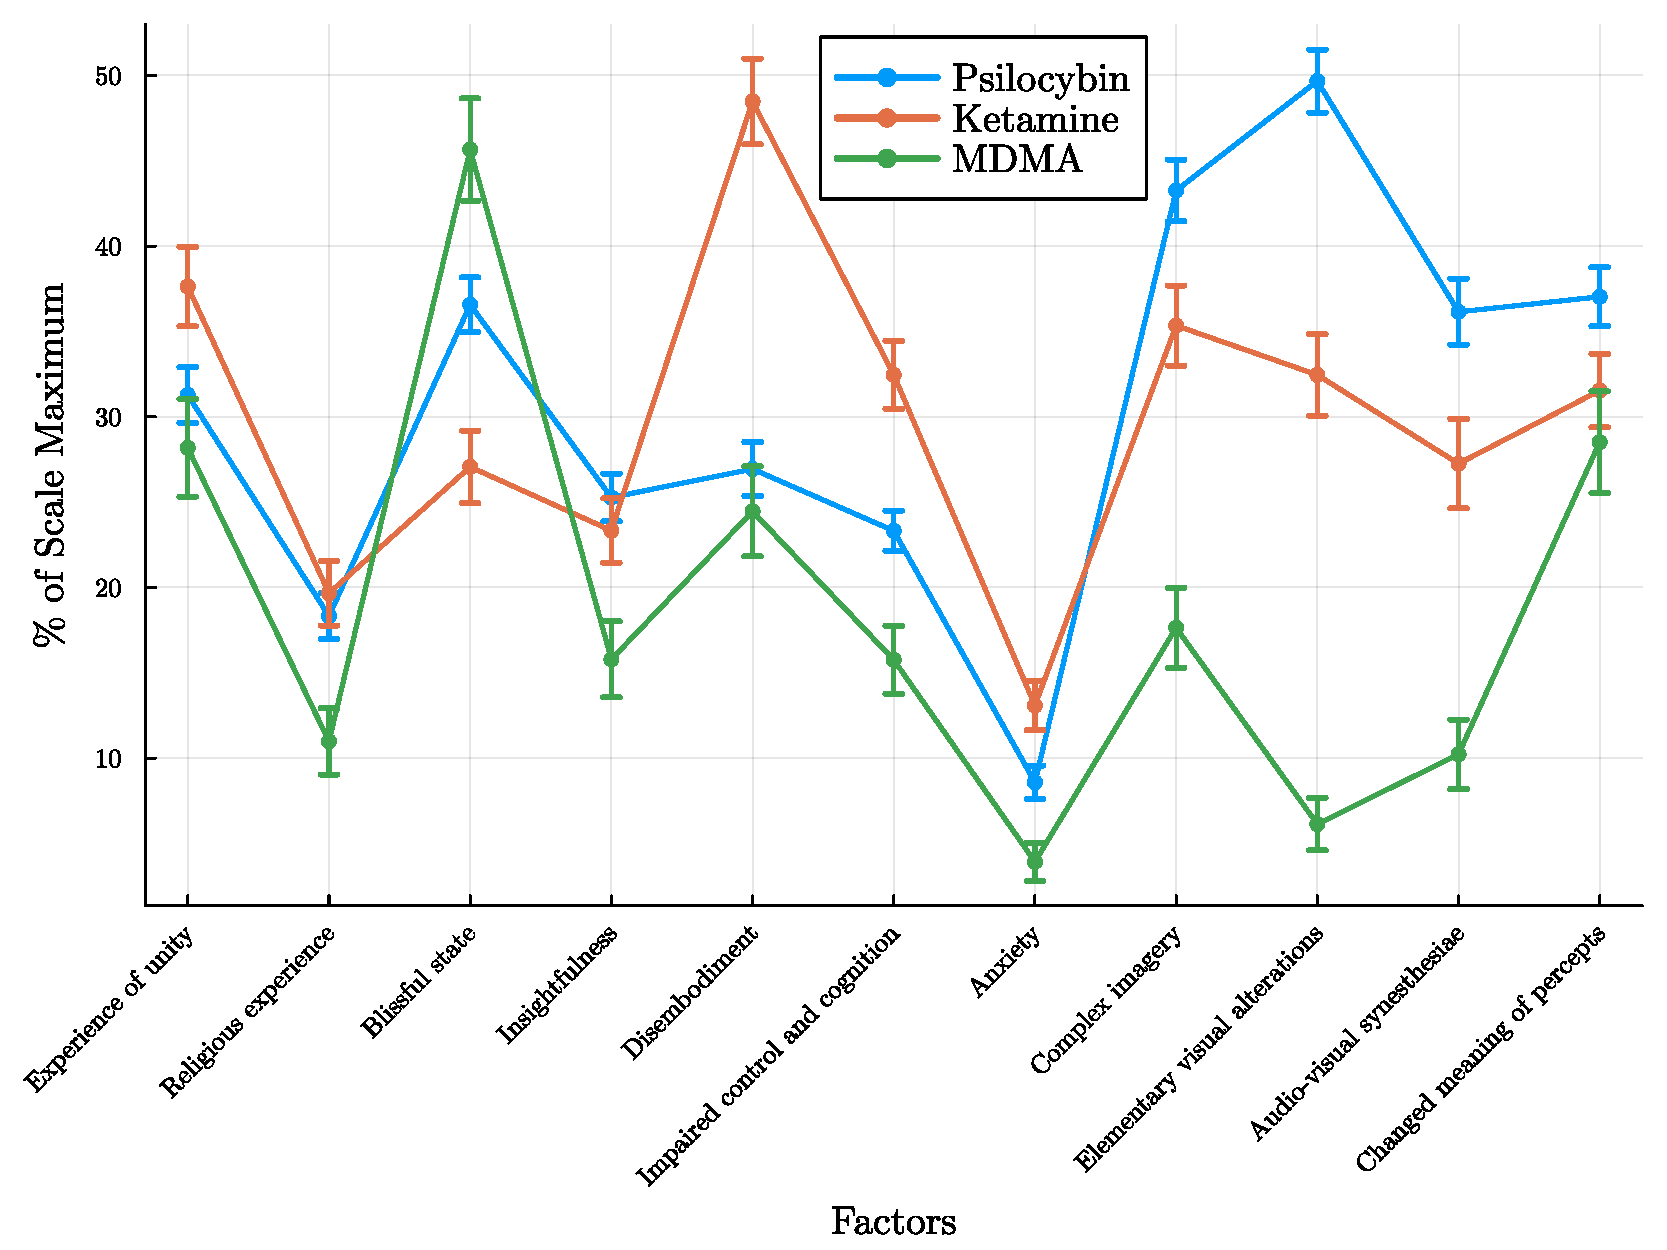
\includegraphics[width=\textwidth]{oavvalidationfigure2data/effects_plot.pdf}
  \caption{Psychedelics' effects on consciousness, as measured by the new OAV factors developed by \textcite{studerus2010psychometric}. Error bars represent standard errors. Figure re-plotted from the data underlying the original Figure 2 in that paper.}
  \label{consciousEffects}
\end{figure}
\FloatBarrier
\subsection*{Drug Interactions}
If you regularly take another medication, we suggest consulting \textcite{liechtiInteractions} (more accessible) or \textcite{sarparastDrugInteractions} (more technical) for recommendations on whether you need to discontinue it for a period of time before or after your session. We don't know enough to specifically recommend this resource, but one psychiatric pharmacist specializing in psychedelics offers consultations and drug-interaction resources \cite{spiritPharmacist}. If your medicine is essential for your health we strongly suggest consulting your doctor on how, and whether, you can safely pause it. They will likely not understand the effects of MDMA, so you may need to provide \textcite{sarparastDrugInteractions} to them. That paper discusses pharmokinetics, metabolism, and various drug interactions. If your medication isn't on one of these lists, you can't access a doctor or pharmacist, and you can temporarily discontinue it with tolerable effects, discontinuing it for 5 drug half-lives\footnote{Each drug has a different half-life, which can be found on \href{https://go.drugbank.com}{DrugBank} under Pharmacology → Metabolism.} before the session and 2 days (5 MDMA half-lives, and also the amount of time required to recover 50\% of baseline CYP2D6 enzyme capacity \cite{omathunaCYP}) after the session would generally ensure that 98\% of a drug has been excreted from your body \cite{andradeHalf,torrePharmacology}. This does not account for health conditions that affect metabolism or other relevant processes. On rare occasions a drug's relevant effects persist even after it has been totally eliminated from your body, as is the case with SSRIs, SNRIs, NRIs, NDRIs, and MAOIs.
\begin{itemize}
    \item Taking MAOIs within two weeks before an MDMA session or within a few days after can cause a deadly effect known as serotonin syndrome \cite{malcolmSerotonin,edinoffInteractions}. Notably, one component of ayahuasca is an MAOI \cite{ruffell2020pharmacological}. Co-use with amphetamines, stimulants, and opioids can also produce serotonin syndrome \cite{makunts2022reported}
    \item SSRIs, SNRIs, NRIs, and NDRIs, highly inhibit the effects of MDMA \cite{feducciaSSRIDiscontinuation}\footnote{\label{ssriRetraction}This paper was retracted because a study therapist sexually abused one trial participant, the researchers knew about this but failed to report it and remove that participant's data from the analysis, and the researchers failed to disclose conflicts of interest \cite{feduccia2024retraction,nytimesRetraction}. These are major ethical breaches. We still cite the paper because it's the only source of rigorous data on this important phenomenon that we are aware of. Additionally, the effect size was so large that one changed data point wouldn't have significantly changed the outcome.}. Long term use of these medications causes this effect to persist long after medication discontinuation. The therapeutic efficacy of MDMA therapy is reduced by half even after 25 days of discontinuation. Further discontinuation may bring further benefits. Discontinuation typically requires multiple additional weeks of tapering to manage withdrawal.
    \item Combining MDMA with other prescription psychiatric drugs can cause a variety of changes to the intensity or duration of various effects \cite{sarparastDrugInteractions}. No generally high-risk interactions, except for MAOIs, have yet been found. However, some may increase low- to moderate-risk adverse effects or decrease the therapeutic effects of MDMA.
    \item The liver enzymes CYP2D6/COMT, CYP1A2, CYP2B6, CYP2C19, and CYP3A4 metabolize MDMA \cite{torreEnzymes,sarparastDrugInteractions}. \textcite{flockartTable} maintains a list drugs that inhibit, enhance, or are metabolized by CYP enzymes. Drugs that enhance CYP enzymes may reduce the intensity and duration of MDMA effects by removing it from your blood at a faster rate. Combining large doses of drugs that are metabolized by CYP with MDMA may overload one of these metabolic pathways and potentially cause problems, though it's unclear which drugs and how much. Drugs that strongly inhibit these enzymes, such as ritonavir, may be dangerous to take with MDMA because they lead to excessively high or long-lasting concentrations in your blood \cite{sarparastDrugInteractions}. Again, the degree of danger is unclear and dependent on a drug's degree of inhibition and dose. Some inhibitors, like SSRI's, don't seem to cause dangerous effects (other than reduced therapeutic benefit) when combined with MDMA. The multiple enzymes provide some redundancy if one pathway is inhibited, making drugs that inhibit multiple enzymes particularly dangerous.
    \item MDMA almost completely inhibits the CYP2D6 liver enzyme, one of multiple parallel metabolic paths for MDMA \cite{omathunaCYP}. This inhibition returns to baseline with a half-life of 47 hours. Thus, about 2 days after a session enzyme activity will be 50\% of the way to baseline, 75\% after 4 days, 88\% after 6, 94\% after 8, and 97\% after 10. This effect may counteract tolerance or lead to unexpectedly strong reactions to subsequent doses MDMA. Inhibited CYP2D6 slows the metabolism of MDMA and a number of other drugs, especially ones that are not metabolized through any other parallel pathways that could take up the slack. Thus, dangerous concentrations of certain drugs could accumulate in your blood when those drugs are used within a few days of MDMA. \textcite{flockartTable} maintains a list of drugs metabolized by various enzymes. Look in the "substrates" section. Even if you aren't taking any medications, the precautionary principle might suggest spacing sessions far enough apart to allow recovery, perhaps a week or two at minimum.
    \item Unregulated pills marketed as MDMA/ecstacy/molly can contain harmful adulterants or different amounts of MDMA than was advertised \cite{saleemiAdulterants}.
\end{itemize}
\subsection*{Medical Considerations}
\begin{itemize}
    \item MDMA increases average blood pressure by 17/6 mmHg and heart rate by 15 b/min in therapeutic contexts \cite{mitchellMDMAClinicalTrial}. Transient increases in systolic blood pressure to above 180 mmHg occurred in 5\% of users in one study \cite{vizeliActuteEffects}. This may be a risk for individuals with cardiovascular disease. Individuals with "...uncontrolled hypertension, history of arrhythmia, or marked baseline prolongation of QT and/or QTc interval" were excluded from clinical trials for this reason \cite{mitchellMDMAClinicalTrial2}. That may not be a complete list of cardiovascular conditions contraindicated for MDMA, and caution should be used for any cardiovascular disorder. It's unclear exactly how much of a risk these actually pose, and clinical trial exclusion criteria are often conservative. A search of the FDA Adverse Event Reporting System found "A total of 17 unique cases were reviewed in this study. There were no reports where MDMA was taken as a single agent and ischemic, hypertensive, or arrhythmic adverse events were reported. All cases included co-use with other medications associated with cardiac function abnormalities \cite{makunts2023concomitant}."
    \item Extremely high lifetime use of psychedelics causes valvular heart disease \cite{droogmans2007valvular,tagen2023valvular}. In one observational study, 28\% of chronic MDMA users showed signs of valvular heart disease (VHD) when evaluated with echocardiography, compared to 0\% in a matched control group who reported no MDMA use \cite{droogmans2007valvular}. The chronic users with clinically significant VHD self-reported a mean consumption of 943 MDMA tablets, while the chronic users without clinically significant VHD reported a mean consumption of 242 tablets. This may give a very rough indication of how much MDMA is needed to cause VHD.
    \item It's unclear what degree of liver function is necessary for MDMA therapy \cite{krausCirrhosis}.
    \item MDMA, like many medicines, may have uncommon, poorly understood side effects, particularly after long-term high-frequency use, or in populations with certain genetic features or health problems.
    \item MDMA commonly causes mild hyponatremia (low plasma sodium concentration) in individuals who drink fluids as desired during the session \cite{atilaHyponatremia,baggottWater}. Not drinking anything, or only drinking a few sips, prevents this problem. Adding salt to the fluid has not been tested as a solution, and is known to not reliably prevent hyponatremia in athletic activities \cite{hew2008statement}.
    \item Prolonged, intense physical activity in high temperatures combined with dehydration can cause dangerous heat illness, as sometimes occurs at dance parties \cite{vanOverheatingAlcohol}. Alcohol co-use also significantly exacerbates the risk of heat illness.
    % \item Planning careful or reduced movement during altered states of consciousness may be advisable if your body is prone to injury from otherwise typical human movement. A sitter, guide, or therapist could help you with this during the session, or you could put an obvious reminder sign in your field of view.
    \item \textcite{kangaslampiAdolescent} saw no obvious reasons why adolescent use would be risky. However, this assumption has not been tested in any trials. Developing individuals could react differently to MDMA than adults. You may have to trade off these unkowns against the fact that treating mental illness is important \cite{mitchellMDMAClinicalTrial}.
    \item As with most problems associated with MDMA \cite{riggDeaths}, seizures are very rarely reported, and when they are, they are mostly associated with mixing intoxicants, extremely high doses, hyponatremia from drinking too much water, or heat stroke from dancing all night without adequate fluid intake \cite{freidelSeizures}.
    \item We couldn't find any high-quality information about using MDMA while pregnant or breastfeeding. The precautionary principal probably indicates that these combinations should be avoided until they are rigorously demonstrated to be safe.
    \item Adequate sleep is likely important for productive sessions and post-session recovery \cite{simon2020sleep}. People commonly experience up to three days of post-session fatigue \cite{liechtiGender}. Starting another session before you have recovered from the previous one may reduce session effectiveness and increase the risk of undesirable effects.
    \item Tolerance to MDMA starts developing within 1–2 hours of ingestion and is a primary reason the effects decline much faster than MDMA's plasma concentration \cite{farreTolerance,parrottTolerance}. We have been unable to find any data showing how long it lasts and distinguishing the effects of tolerance from dissociation, avoidance, or the natural variation of sessions may be difficult. We suggest spacing sessions further apart or reducing dose if you notice a pattern of diminishing effects. Using higher and higher doses to overcome tolerance will produce negative effects.
\end{itemize}
\subsection*{Psychological Risks}
\begin{itemize}
    \item Psychological destabilization (see Section \ref{sec:complex}) is a common occurrence in therapy \cite{olthofDestabilization}. It's associated with better outcomes later in therapy, but if it is intense enough and not managed well can severely interfere with your life. We are not aware of any papers demonstrating this, but we think it's likely that psychedelic therapy tends to produce stronger destabilization (and more rapid therapeutic progress) than traditional psychotherapy. We suspect severe early childhood trauma (including non-secure attachment) is a major risk factor, but this is hard to assess. The therapeutic alliance is an important mitigating factor when working with a mental health professional (see \textcite{BRWAIdownload} for an assessment scale) \cite{fluckiger2018alliance}.
    \item Possession of multiple doses may be risky for those with severely impaired impulse control if they see the medicine as an escape, an immediate drug-based solution that doesn't require a therapy component, or don't understand the need to recover between sessions. They may use too high of doses, use it too frequently, or use it in unsafe contexts.
    \item Altered states of consciousness and post-session exhaustion can impair awareness and reaction times. Avoid driving and other potentially risky activities on the same day as the session.
    \item Complex or compelling distortions of external reality on MDMA are rare and correlated with unusually-high doses, but people more commonly have closed-eye visuals (possibly involving traumatic events they experienced) \cite{liechtiGender}. These visuals may be symbolic instead of a realistic reliving. Temporary and mild visual changes such as color and texture enhancement are common. Sometimes psychedelics, along with many other psychoactive drugs, trigger persistent visual distortions or anxiety about existing but unnoticed visual distortions \cite{alexanderHPPD,halpernHPPD}. When this causes significant distress or impairment it is called Hallucinogen Persisting Perceptual Disorder (HPPD). HPPD is strongly linked to pre-existing anxiety or dissociation, and often improves as those are treated. HPPD from MDMA is unrecorded in clinical trials, but some recreational users report it \cite{vizeliActuteEffects,litjensHPPD}. One survey found that when people do report persistent visual or auditory distortions (from any psychedelic), 73\% say "they [the symptoms] don't bother me at all", 24\% "I'd rather not have them, but I can live with them", 0\% "they irritate me", and 1\% "they drive me mad \cite{carhart2010user}."
    \item Suicidal ideation: MDMA therapy with high levels of support decreases suicidal ideation about as much as placebo with therapy, on average \cite{mitchellMDMAClinicalTrial,mitchellMDMAClinicalTrial2}. When interpreting these results it is important to note that average improvements can mask the possibility that a small portion of individuals can get worse even while the majority improve, though this applies to the placebo group as much as the MDMA group. Suicidal ideation is part of the biopsychosocial complex system of mental health. Our impression is that psycho compontent is heavy since suicidal ideation almost always involves accompanying schema-like beliefs. Suicidality can presumably get worse for a period of time like many other schemas during the reconsolidation process.
    \item Mania: There is virtually no high quality experimental data because people with a history of mania (less-so hypomania) are usually excluded from clinical trials of psychedelics \cite{gardBipolar}. The MDMA phase III trials did not exclude individuals with bipolar II and no manic episodes were reported \cite{mitchellMDMAClinicalTrial2}. One small, uncontrolled study of psilocybin-assisted therapy for people with bipolar II but not currently in a hypomanic state showed good efficacy and safety when combined with a high level of support \cite{aaronsonBipolarII}. We aren't sure how well that translates to MDMA therapy. Notably, we couldn't find a single case report of mania where MDMA was unambiguously involved in the recent past, and are therefore confused why MDMA and disorders involving mania are often considered a risky combination. Perhaps it is because bipolar I frequently also involves psychosis, which does have a link to MDMA use.
    \item Psychosis: There is virtually no high quality experimental data because people with a history of psychosis are usually excluded from clinical trials of psychedelics \cite{la2022Psychosis}. There are a number of case reports of psychotic episodes induced by MDMA thought they typically, though not always, report confounding factors like co-use with other psychoactive drugs, chronic abuse of other drugs, lack of verification of MDMA ingestion, heat stroke, hyponatremia, extreme doses, or extreme frequency of use \cite{psychosisTreatment,arnovitzSchizophrenia,mcguirePsychosis,patelPsychosis,vaivaPsychosis}. One participant out of 174 in the MDMA phase III clinical trials reported a psychotic episode after the trial ended in poorly-documented circumstances \cite{powerTrip}, even though participants reporting any personal history (family history was allowed) of psychotic disorders were excluded from participation \cite{smithSystematic,mitchellMDMAClinicalTrial2}. We have heard two reliable anecdotes of high-dose psilocybin trips done the day after an MDMA therapy session causing a psychotic episodes. This suggests a lack of adequate recovery between sessions is a major risk factor. This is unsurprising given that high doses and frequent use of a wide range of psychoactive drugs is a well-established risk factor \cite{drugsPsychosis}. \textcite{psychosisTreatment} found that when psychedelics were implicated in psychotic episodes, the episode lasted an average of 1.8 weeks with antipsychotic treatment.
    
    Like other mental illness, psychosis is a complex biopsychosocial phenomenon. We've seen a few self-reports from people stating that a single MDMA therapy session triggered a psychotic episode. We've also seen 4 reports from people stating that an MDMA therapy session resolved an existing psychotic episode. Additionally, we know of a few cases where people have safely used MDMA therapy despite previous psychosis, even when psychedelics were major factors in the psychotic episodes. This suggests that schema's and/or stress play a significant role in these psychotic episodes.
\end{itemize}

\textcite{evans2023extended} surveyed people who have experienced new, persistent negative symptoms after recreational, professional-therapeutic, and DIY-therapeutic psychedelic experiences. This data applies to all psychedelics, not just MDMA. Most symptoms dissipated with time, but 17\% of respondents said theirs lasted more than 3 years. From most to least common, participants reported emotional (76\%), self-perception (58\%), cognitive (52\%), social (52\%), ontological (50\%), spiritual (34\%), perceptual (26\%), and other (21\%) difficulties. There is major uncertainty in how much these symptoms are due to \cite{calder2025traumatic}:
\begin{itemize}
	\item Surfacing of existing maladaptive schemas and subsequent defense cascade activation, a necessary and healthy part of the therapeutic process if managed well. You may have been avoiding these schemas until the session. \textit{We think there is a high likelihood of this for MDMA therapy. It's conceivable that a highly skilled therapist could help you keep to destabilization in small, easily dealt with chunks, but psychedelic experiences are famously difficult to control.}
	\item Trauma from life impairment or destabilization due to poorly managed surfacing of maladaptive schemas and trauma. \textit{This is possible, though the risk can be significantly reduced with assistance from mental health professionals with whom you have good therapeutic alliance (see \textcite{BRWAIdownload}) \cite{fluckiger2018alliance}.}
	\item Trauma from the psychedelic experience itself. \textit{We think this usually results from large doses of hallucinogens, unsafe settings, and abusive or incompetent guides/therapists. Traumatization risk may be low for MDMA itself because of its intense feelings of safety and low hallucinatory and spiritual effects \cite{studerus2010psychometric}.}
	\item Difficult or destabilizing changes to your understanding of self, existence, or meaning. \textit{We think MDMA only rarely induces this because MDMA tends to produce much lower levels of ego-dissolution and mystical experiences than other psychedelics \cite{mdmaExtendedEvans,holze2020distinct}.} See Subsection \ref{selfinsight} for more information.
	\item Something else. We don't know if this exists, and if it does, what it is or how often it occurs.
\end{itemize}
Even in this subgroup of people who experience extended difficulties in the previously mentioned study, 90\% agreed with the statement "I believe that the insights and healing gained from psychedelics, when taken in a supportive setting, are worth the risks involved \cite{evans2023extended}." However, it is possible that a population of psychedelic users who experience debilitating effects was missed due to sampling bias. Psychedelics can also inflate feelings of meaning, potentially biasing respondents to report that their experiences were more valuable than they actually were \cite{hartogsohn2018meaning}.% A similar study using a different set of categories found that those with adverse symptoms from psychedelics had: sense of social disconnection (72\% of study participants who reported adverse symptoms), anxiety and panic attacks (68\%), existential struggle (65\%), feelings of depression (61\%), derealization (55\%), diminished self-esteem (50\%), depersonalization (37\%), sleep problems or nightmares (35\%), difficulty with thinking clearly (33\%), paranoia (21\%), visual hallucinations/disturbance (21\%) \cite{robinson2024investigation}.

\subsection*{Other Common Concerns}
\begin{itemize}
    \item \textbf{Discomfort with Drugs}
        While MDMA therapy is not for everyone, healing can happen even when discomfort is present during a session because MDMA rewrites patterns of (maladaptive) discomfort that you stay present with \cite{fedduciaMDMAMemoryReconsolidation}. Your fear of MDMA could be unlearned if it is not an accurate representation of reality \cite{eckerUnlocking}.
    \item \textbf{Loss of Control}
        While engagement with distressing memories can be intense, people regularly have clear, complex, and emotionally nuanced conversations on MDMA \cite{colbertEvenings,passieHistory}. MDMA creates intense feelings of compassion and safety that make aggressive behavior unlikely. \textcite{nuttDrugHarms} ranked drugs by expert perception of "Harm to others", and MDMA was ranked at about 2\% the risk of alcohol.
    \item \textbf{Drug Stigma}
        Many drugs are harmful, however, during the War on Drugs a wide variety of psychoactive substances were further stigmatized and categorized as harmful without clear evidence-based distinctions regarding their actual risk \cite{alexanderNewJimCrow,nuttDrugHarms}. While there were complex motivations for the War on Drugs, it functions and persists primarily as moral panic, a means to punish certain groups of people, and a means for politicians to disenfranchise and ostracize the voter base of their political opponents. There is little correlation between the legality of psychedelics and their potential for harm \cite{nuttDrugHarms}.
    \item \textbf{Addiction}
        A panel of medical experts organized by the Dutch government found no cases of MDMA addiction in Dutch treatment centers and concluded that "It does not, or only minimally, lead to abuse, dependency or use-related disorders \cite{netherlandsMDMA}." Withdrawal has also not been found in rodent studies, even at extreme dosing schedules \cite{robledoDependence}. However, MDMA, like most experiences that can make you feel profoundly safe, can be psychologically addictive when it is used to escape from difficult feelings rather than engaging with them. Reports of behavioral MDMA addiction in recreational contexts exist, but as previously stated, seem rare and associated with escapism \cite{erowidAbuse}. As previously discussed, there have been many flaws in studies on MDMA abuse. Consequently, little is known about the effects of abusing MDMA, or what level of use causes physical or psychological problems. If you are worried about your potential for addiction, we suggest: only possessing one dose at a time, only obtaining MDMA from a trusted mental health professional who can monitor your abuse potential, don't escalate dosing, don't do solo therapy, and only use it for therapy. We suggest attempting to shift the content of your sessions from escapism to engagement with maladaptive schemas if you're addicted and can't stop. That would make the sessions less rewarding and facilitate improved mental health, which even might resolve the addiction.
    \item \textbf{Neurotoxicity}
    	Some observational human studies and controlled high-dose animal studies have found that MDMA use is associated with neurotoxcicity (oxidative stress in this case) or cognitive problems \cite{passieHistory}. However, these problems have not been found in controlled studies in humans. The human observational studies that find problems usually fail to adequately control for multiple-drug use, a significant risk factor. Notably, \textcite{halpernMormonRavers} ruled out high levels of long-term cognitive issues from recreational MDMA use in a population that had exceptionally low lifetime use of other psychoactive substances. Unfortunately the study didn't have the statistical power to rule out low-moderate levels of cognitive issues. One small randomized study of MDMA therapy also did not find any significant cognitive effects \cite{mithoeferSafety}. The animal studies that found problems typically used extreme doses, extreme frequencies of use, or injected the medicine, a more potent method of administration than swallowing a pill \cite{passieHistory}. It's also not clear that humans respond the same way as rats to an equivalent dose. It's possible that replicating these conditions of extreme doses or frequency of use could cause harmful neural oxidative stress in humans. Some studies have found serotonin system changes in humans, but the studies use a poorly controlled cross-sectional observational design \cite{van2022serotonin}. So it's not clear that MDMA, rather than other drug use or population difference, causes these changes, that the changes are bad, or that the changes are clinically significant even if they are bad. The changes appear to decrease with abstinence. Fear and misinformation about MDMA is widespread due to the War on Drugs, sensationalized of poor quality research, and misattribution of MDMA-related deaths as an inherent risk of MDMA instead of its interactions with certain medications and health conditions, and the risks of heat illness or hyponatremia at raves \cite{passieHistory}. See chapter "The Toxicity Debate" in The History of MDMA by Torsten Passie for a comprehensive review of the topic.
	
        High doses of certain antioxidants, including alpha-lipoic acid, ascorbic acid, and acetyl-L-carnitine, administered shortly before and during the session, prevent oxidative stress in rats \cite{aguirre1999alpha,shankaran2001ascorbic,alves2009acetyl}. Some companies bundle these antioxidants together in commercially available products, but we are not aware of them having been rigorously tested for usefulness in humans \cite{rollKit}.
    \item \textbf{Misuse}
        We are not aware of any clear evidence suggesting that recreational use of MDMA is problematic as long as the safety considerations in this section are taken into account. One panel of drug-misuse experts estimated that, even in typical non-therapeutic contexts where users are likely not as cautious as they should be of risks, MDMA poses a significantly lower overall health risk than marijuana, and far less than alcohol \cite{nuttDrugHarms}. While those drugs can be used in harmful ways, they can also be used responsibly with negligible negative effects. It is important to note that possession of MDMA is a felony in most of the world, though in practice many jurisdictions do not enforce or prioritize charges for possession of small amounts \cite{alphaLegalization}. We recommend the assistance of an ethical, well-matched, and skilled therapist for anyone who develops a pattern of harmful, escapist, or psychologically-addictive MDMA use. If someone is unable to stop it may help to shift the content of the sessions from escapism to engagement with maladaptive schemas. That would make the sessions less rewarding and facilitate improved mental health, which even might resolve the addiction.
    \item \textbf{Origins of MDMA}
        MDMA (Figure \ref{fig:mdma}) is generally made by making several modifications to the plant compounds safrole (Figure \ref{fig:safrole}) or piperonal (Figure \ref{fig:piperonal}) \cite{worldDrugReport,euMDMA}. When properly conducted, this process results in pure MDMA. Single-substance purity greatly improves the ability to produce accurate and safe doses. Refer to \textcite{ruggeriNatural} for a nuanced discussion of what "natural" means. For those concerned about the pharmaceutical industry: MDMA was first made in the early 20th century by Merck as an intermediate product with no recognized use itself \cite{passieHistory}. The first known human use of MDMA was in the early 1970s as a legal alternative for MDA in recreational use. Its first use in therapy occurred in the late 1970s after the independent chemist Alexander T. Shulgin realized it's therapeutic potential and introduced it to the therapist Leo Zeff Ph.D., who used it with many clients and taught many therapists how to use it. Then, once it was made illegal, legal therapeutic use ended. Making it legal again would require enormous amounts of money to run proper FDA-approved clinical trials, but no regular drug company was willing to do this because the original patent expired in the 1930s, and they wouldn't be able to recoup their investment through drug sales. The 21st century clinical trails were funded through a combination of 1) donations to the nonprofit Multidisciplinary Association for Psychedelic Studies (MAPS) and 2) MAPS selling shares of its for-profit division Resilient Pharmaceuticals (previously known as Lykos) \cite{lykosPatents}. To recoup their investment Resilient tried to patent a specific particle size of MDMA crystals within a pill, but the patent office rejected it. Their business plan is now unclear. We think that in 2025, outside rare clinical trials or limited legal use in certain countries, all MDMA used in therapy is ultimately sourced from underground chemistry labs and has nothing to do with Resilient or MAPS.
        \FloatBarrier
        \begin{figure}[htbp]
            \centering
            \chemfig{*6(-=-(--[::-60](-NH-[::-60])-[::-60])=-(*5(-O--O-))=)}
            \caption{Structure of MDMA.}
            \label{fig:mdma}
        \end{figure}
        \begin{figure}[htbp]
            \centering
            \chemfig{*6(-=-(--[::-60]=[::60])=-(*5(-O--O-))=)}
            \caption{Structure of Safrole.}
            \label{fig:safrole}
        \end{figure}
        \begin{figure}[htbp]
            \centering
            \chemfig{*6(-=-(-=[::-60]O)=-(*5(-O--O-))=)}
            \caption{Structure of Piperonal.}
            \label{fig:piperonal}
        \end{figure}
        \FloatBarrier
    \item \textbf{Can I Inadvertently Unlearn a Healthy Schema?}
        \label{unlearnHealthy}
        As stated by \textcite{ecker2015misunderstood}:
        \begin{quotation}
         When two mutually contradictory schemas are juxtaposed consciously, the schema that more comprehensively or credibly models reality, and therefore more usefully predicts how the world will behave\footnote{The phrase "predicts how the world will behave" may be confusing here, but it includes beliefs about yourself (e.g. I am good, I am bad) and how you react in various situations (e.g. dogs are threatening enough to trigger a fight-or-flight reaction).}, reveals the other schema to be false, and the falsified one is immediately transformed [reconsolidated] accordingly.
        \end{quotation}
        The reconsolidation process doesn't imply that your post-reconsolidation beliefs will be a precise truth about the world or yourself, only that it will be more true than the falsified/unlearned schema in the context of your lived experience. We think this generally produces good outcomes, but is not perfect. There might be rare situations where a healthy but false-according-to-your-lived-experience schema is unlearned. For example, someone's especially deep desire to not be alive might be able to contradict their desire to, say, avoid falling off cliffs. In that case their avoid-falling-off-cliffs schema would be an unintegrated remnant from a time in their life when they did want to be alive. In case such a scenario is actually possible, please do not try to unlearn any schemas critical for keeping you or any other being safe. Do not conduct MDMA therapy in acutely dangerous situations where healthy danger avoidance schemas may activate. We are also hopeful that using MDMA's compassion, connection, and safety to facilitate reconsolidation of one's own fears and insecurities also tends to result in schemas that are associated with more compassion, connection and safety. On a practical level, we are unaware of any instances of MDMA therapy unlearning a fundamentally healthy schema. The closest example we are aware of is the unlearning of fear-based schemas that, while unhealthy, may temporarily provide some necessary functionality in your life (see Section \ref{sec:complex}).
        
        Similarly, the reconsolidation process can't always help you unlearn erroneous beliefs that were formed from unrepresentative sets of experiences. If you were the first human to meet aliens, and they attacked you, you might reasonably learn "these aliens are dangerous," and no amount of reconsolidation will change that until you acquire contradictory knowledge (maybe you learn that that alien happened to be a pirate and all the other aliens are very nice people).
\end{itemize}
\section{Professional Guidance vs. Self Guidance}
\label{professionalVSSelf}
MDMA therapy can succeed in a wide variety of contexts including therapist-guided sessions with pre- and post-session support, do-it-yourself couples therapy, and solo therapy \cite{mitchellMDMAClinicalTrial2,colbertEvenings,hillsSolo}. However, we believe working alone with MDMA presents higher risks and a lower healing likelihood compared to partnering with an ethical, skilled, and well-matched therapist or guide. However, that may not always be the best option available because it is often difficult and expensive to access an ethical, skilled, and well-matched therapist or guide. Many people have also had a variety of negative experiences with mental health professionals and reasonably don't want to interact with one. Per our individual and clinical experience, an ethical, skilled, and well-matched therapist or guide may provide:
\begin{itemize}
    \item A trustworthy presence that creates a greater feeling of safety, enabling more effective healing
    \item Additional perspective that's hard to see from a first-person view
    \item Education on trauma, healing, trust, what healthy relational patterns look like, and healthy ways to deal with emotions
    \item Troubleshooting for problems with the medicine or other parts of the healing journey
    \item Improved screening for conditions that might make MDMA particularly risky for an individual
    \item Monitoring of your level of destabilization over time
    \item A skilled and experienced perspective about how best to maintain your to your window of tolerance, and broaden your window of tolerance over time
    \item Assistance in learning appropriate coping strategies
    \item Assistance identifying which coping strategies are best for you in a particular context
    \item Assistance preparing executive function supports for yourself to maximize your capacity to use the right strategies at the right times
    \item Management of destabilization periods to reduce disruptions to your life–including empathetic encouragement to rest or cut back from other obligations when appropriate, in order to preserve over-all wellness and capability, and assistance strategizing ways to manage your life that will minimize disruption 
    \item Guidance through difficult therapeutic exercises
    \item An empathetic and grounding presence while you think through major life decisions, relational challenges, and challenging new schemas that may emerge in the course of the work
    \item Assistance identifying supplementary treatment modalities that are likely to be most effective for your situation, and in some cases, information about how best to access those treatment modalities
    \item Assistance in planning for your medicine experience and organizing appropriate social support for the whole process
    \item Unadulterated medicine and/or some degree of medical monitoring, depending on who you're working with
\end{itemize}
Therapists and guides who are ethical and skilled but whose style or personality are not a good match for you should be easy to approach about this mismatch, and they should recommend any colleagues who they think would be a better match. We think the risks inherent in working with an ethical and skilled therapist or guide who you don't match well with mostly involve wasted time and money, and possibly demoralization. However, we think the risks of unethical or unskilled therapists and guides can include:
\begin{itemize}
    \item Emotional, physical, financial, or sexual abuse \cite{powerTrip}. This includes Adverse Idealizing Transference (see Subsection \ref{def:ait}).
    \item Excessive dependence on that therapist or guide \cite{powerTrip}
    \item Increased risk of adverse effects and destabilization, possibly though overly intense or frequent psychedelic sessions with inadequate support.
    \item Ineffective treatment that the mentally healthy would find frustrating could be totally demoralizing to the mentally unhealthy.
    \item They may push their own interpretations on you while you are in a suggestive state of consciousness, potentially leading to false beliefs of abuse \cite{Scoboria07022017} or false beliefs about how trauma and mental illness work.
\end{itemize}
\label{suicideCops}
Furthermore, licensed mental health providers are usually legally obligated to call the police on you if they think you are at high risk of suicide or hurting someone else. What level of risk your provider thinks is sufficient to call the police is strongly dependent on their individual judgement, personal interpretation of local laws, how much they fear being sued or losing their license if someone dies or gets hurt and then blames them, and how much they believe involuntary hospitalization will help you. If you are suicidal or fantasize about hurting your abuser, we strongly suggest asking your provider to elaborate their decision criteria before you meet with them, or during your first appointment before they ask you if you are suicidal or want to hurt someone. Then you can decide if you can cope with the level of self-censorship necessary to stay outside their boundary. Or, you may even trust your provider enough that you can be completely open with them because you know they will only tell you to go to the hospital if you really need it. In that case you could write up a crisis plan involving which hospital you want to go to, which family members or friends you want notified, etc. If your provider does call the police on you, know that police typically have little training in the mental health and will likely take your provider's word over yours. There is also a good chance that the police dragging you away against your will to a place you can't leave-where medical staff may do a variety of invasive and non-consensual things to you-will traumatize you. Even worse, \textcite{emanuelHospitalization} found that (in Allegheny County) involuntary hospitalization significantly increases the chance of a patient killing themselves or hurting someone else over the 6 months following admittance in cases where clinicians might disagree about admitting a patient (43\% of evaluations in this study). It's not clear how well these results apply to situations where multiple clinicians would all agree on admitting a patient. \cite{emanuelHospitalization}. We think \textcite{alexanderInpatient} is a good guide for navigating/avoiding the inpatient mental health system.

Individual and couples MDMA therapy without professional assistance (possibly with the assistance of a trusted, empathetic, and emotionally non-reactive sitter \cite{thalSitter}), appears to work well for some people, including the author M.G. \cite{hillsSolo,colbertEvenings}. We are uncertain what circumstances lead to positive vs. negative experiences, or the degree to which various risks are increased. We can't say if this is appropriate for your particular situation, but it is an option that a lot of people like for various of the reasons listed in this section.

We propose the following ranking of options. The top of the list represents the lowest risk of adverse outcomes, the highest likelihood of durable healing, and also the highest financial cost. This list is a general guide and the exact positions of items are debatable, as well as dependent on personal circumstance. Exceptions to the rule always exist.
\begin{enumerate}
    \item Continually working with a skilled, ethical/accountable, psychedelic-trained therapist or guide you align well with. \textit{We tentatively think this is the ideal model for most situations if you can find the right clinician to work with and have enough money. We also think this model is especially important for people with potentially dangerous symptoms they can't manage themselves, possibly including psychosis, mania, suicidal ideation, or a severe lack of impulse control.}
    \item Start off with a skilled, ethical/accountable therapist or guide who you align with and who is psychedelic-trained and/or personally experienced with MDMA. You may later transition to self-guided sessions (with regular check-ins) if you and your clinician collaboratively decide that you are ready. \textit{This model has not been explored in the research and may have a higher risk of difficulties. However, some people pursue this method because it offers dramatically lower costs and there are many anecdotes of people (including the author M.G.) who have found it highly effective.}
    \item Work with a skilled, ethical/accountable non-psychedelic-trained therapist or guide you align well with; collaboratively assess your risk-factors with them. You might read the safety section of this guide together, or consult with a psychedelic trained therapist. If your risk factors are low, you then self-guide all your medicine sessions while maintaining regular sessions with your clinician. You also use high quality resources (see Section \ref{sec:psychoeducation}) to educate yourself on the nuances of effective and safe MDMA therapy and use a high-quality sitter as appropriate, which includes at least the first several sessions (see Section \ref{def:sitter} for characteristics of good sitters). \textit{We think this model is similar to the previous one, but–depending on the quality of your self-education–somewhat more difficult and riskier.}
    \item Self-guide all your medicine sessions and do all of your own between-session work, perhaps talking about your healing journey with emotionally skilled friends or friends skilled in safely using psychedelics for healing. You also read high quality literature (see Section \ref{sec:psychoeducation}) on trauma healing and use a trusted sitter for at least the first few sessions (see Section \ref{def:sitter} for characteristics of good sitters) \textit{We don't generally recommend this model because self-assessment of risk factors is very difficult. If you do try it, we think you will greatly benefit from high self-emotional knowledge and high skill in managing your own emotional reactivity. While this model has worked for many people, we are unsure of the risk/benefit trade off. We strongly recommend identifying and at least briefly connecting with a therapist or guide you might want to work with in case you get into deeper water than you are comfortable with.}
    \item Self-guide all your medicine sessions and do all of your own between-session work. You don't use any high quality reference material and don't understand the nuances of safe and effective healing. Or you work with an incompetent or abusive guide or therapist who may harm you by suggesting overly-intense psychedelic sessions and not effectively help you with the resulting trauma or destabilization. They may also offer distorted or unhealthy interpretations of experiences you have during a session. \textit{We don't recommend this in any circumstance. While it is occasionally helpful to some, we think the lack of rigorous understanding of the process can place both safety and healing at elevated risk, and is likely to impair healing to some degree. Adverse effects may not be identified, understood, and well-managed}.
\end{enumerate}
It seems important to note that although more data is needed, therapeutic use of psychedelics in professionally supported group sessions, where multiple therapists look after a larger number of clients throughout a medicine experience, may offer a potential way to make professional support more accessible \cite{marseille2023group}. It also likely comes with it's own set of poorly-understood risks.

\section{How to Find a Therapist or Guide}
\label{sec:howtofind}

Which therapist you work with matters a lot. For instance, in a large study done by \textcite{firth2019therapistEffects}, after adjusting for demographic factors (like the severity of symptoms clients were entering therapy with), the best 3.9 percent of clinicians had 77.2 percent of their clients recover; the recovery rate for therapists in the average range was 58 percent; and the 3.9 percent of clinicians who had the worst outcomes only saw 41.4 percent of their clients recover (Note that a significant percentage of people recover even without therapy, so it's possible that the worst therapists have a negative influence on their clients.).

It is our hope that the following recommendations, which largely emerge from our personal and clinical experience\footnote{This experience includes some common knowledge of professional norms among the licensed mental health professions, much of which can be found in the ethics codes of the major licensed mental health professions, e.g. the National Association of Social Workers code of ethics, the American Psychological Association code of ethics, the American Counseling Association code of ethics, The American Association for Marriage and Family Therapy code of ethics, etc.}, can make finding a therapist feel less overwhelming and more hopeful for those who are struggling–or who don't even know where to start–with the search.

First, we acknowledge the difficulty: even under optimal circumstances, accessing mental healthcare can turn out to be a slog. These challenges are common knowledge for people who provide community mental health services and/or who have accessed them repeatedly: the financial and administrative costs are often daunting. Interacting with licensed mental healthcare professionals is inherently vulnerable for many, especially those who have witnessed or experienced carceral hospitalization or forced medication. Intake interviews often demand intimate details of one's finances, sexuality, and medical and mental health. All of this is the price of accessing a clinical relationship that may or may not be very helpful. If it isn't, clients may feel they need to stick with it, because they do need help, and finding someone else to help them seems like more than they can take on, but that doesn't necessarily mean the clinician will stick around–and particularly for those who are using Medicare/Medicaid or who require less-expensive sliding scale services, clinicians may be students whose clinical internships end only a few months after starting to work together. Online services, which have endeavored to bridge the gap between what is needed and what is easily available, are plagued by serious ethical and product-quality concerns \cite{betterhelp1,betterhelp2,betterhelp3,talkspace1,doneglobal1}.

The good news is that there \textit{are} excellent clinicians out there–and not all of them are late in their careers. Early career therapists, like those who tend to staff more affordable clinics, provide just as good of care as their more experienced counterparts \cite{goldberg2016psychotherapists}. Here are our recommendations on how to find one that's right for you.

\subsubsection*{Bad Therapy is Worse than no Therapy}
Remember that really bad therapy can really hurt you \cite{hook2018boundary}, and as such we feel it is worse than no therapy. Bad therapy can leave you stagnant for a long time with the impression that no real help for you exists. It can make your symptoms worse without making them better after. In the worst case scenario, it can leave you with additional trauma. See Subsection \ref{sec:mdmaTherapistComplications} for a discussion of the particular challenges of avoiding negative and damaging clinical experiences in the realm of psychedelic therapy.

Good therapy is often very uncomfortable \cite{eckerUnlocking}. However, you should feel a sense of mutual trust and respect with your clinician, and you should also feel a sense of collaboration and consent regarding the goals you are working towards and the methods you use to get there \cite{BRWAIdownload}. Even if you don't understand the methods your clinician is using to help you, we believe a skilled and well-matched clinician will take the time to help you develop a trust in them that is commensurate with the discomfort of what they are asking you to undertake.

Although we cannot speak to the specific trade-offs of your situation, in general we recommend continuing to search until you are able to access good therapy.

\subsubsection*{Trust your Personal Experience}
Trust your perceptions, because your personal experience of your clinician impacts the efficacy of your treatment \cite{horvath2011alliance}. You don't just need a good provider, but a good provider who is also a good fit with you. We strongly recommend using the BR-WAI \cite{BRWAIdownload}, an empirically validated tool for understanding how you and your therapist are connecting, and what might be required to improve that connection.

In our experience, it's a good idea to look for someone it feels like you could say anything to. If you cut your arm, any skilled emergency physician will be able to competently stitch you up. The same is not true with a comparable degree of psychiatric injury \cite{firth2019therapistEffects}. In mental healthcare, the bedside manner is part of the intervention, and the same bedside manner doesn't work for everyone. Although the most skilled mental healthcare providers connect well with an extremely broad spectrum of clients, it is unrealistic to expect every provider to "click" with every client–and many excellent mental healthcare providers ultimately focus narrowly on particular populations of interest to them. If you aren't connecting with a particular clinician, it doesn't mean anything is wrong with them, and it doesn't mean anything is wrong with you.

\subsubsection*{Feedback}
Good therapists love feedback and direction. It is very likely that many therapists who could do great work with you if you are expressive about what you need and want would, in contrast, be very bad therapists for you if you aren't expressive about those things \cite{macdonald2015correcting,delgadillo2022progress,lambert2001effects,oanes2015therapists}. If you can, we recommend asking clearly for what you want and talking clearly about how things feel. Additionally, there are several instruments that have been developed to help therapists measure and improve their performance. Examples include the BR-WAI, the ORS-SRS, the Core-OM, or the QR-45.2. If your therapist asks you to participate in one of these formal feedback mechanisms, we recommend doing so, even if it feels awkward; these measures really seem to help therapists provide better services.

We've observed that it is sometimes helpful to imagine what therapy would be like, if it went as well as you could possibly imagine, and to share this with your clinician–and to articulate your fears about the process. You can also ask if your ideal hopes align with their experience of their methodology, which may help you set expectations for your treatment. You can use the list above (of what a skilled therapist can provide) to identify ways you would like your therapist to support you. It may be helpful to identify which forms of support you are interested in receiving, and to spend some of your initial sessions learning how your clinician feels about providing support in those particular ways.

Particularly if you have been working with a particular clinician for a while and your issues/diagnoses and demographic are within their main practice area, you are \textit{well} within your rights to ask a clinician to go outside their comfort zone to learn or implement a new-to-them intervention that is right for your situation. An accredited therapist is required to complete continuing education hours anyway. There are lots of legitimate reasons they may say no (cost, time, and accessibility of additional training, to start with), and that's OK too–but please don't be afraid to ask.

If things aren't working, and you've made some effort to recruit your clinician's help in fixing the situation, a therapist may also be willing to spend some of your final few sessions helping you find and connect with someone who is a better fit for you.

\subsubsection*{Boundaries}
\label{def:ait}
Good therapists have good boundaries. Clients often come to therapy without an understanding of what healthy therapeutic boundaries are and why they might be important, and that's OK–it is the clinician's job to have this knowledge, to share it with the client, and to assert boundaries as needed.

One of the most important reasons boundaries are crucial in therapy is a phenomenon called Adverse Idealizing Transference (AIT) \cite{hook2018boundary,transferranceLoveHarm}. Idealizing Transference is a phenomenon in which clients develop strong positive feelings towards their therapist. This can be totally healthy and extremely helpful to the course of therapy–supporting clients in their sense of safety and their ability to sustain focus and effort through the sometimes severe discomfort of healing. However, in some cases, it is possible for these positive feelings to be so strong and misdirected that they cause considerable harm–causing lasting distraction and disruption in the client's life, potentially continuing for decades. This situation creates a severe vulnerability that the therapist, if they are unscrupulous or unskilled, may exploit (intentionally or not) for emotional, sexual, or financial gain–creating severe trauma for the client and sometimes impacting others as well. In these cases, Idealizing Transference has become Adverse Idealizing Transference. Just as helpful medications sometimes have side effects for a small percentage of the people who use them, a small percentage of therapy consumers experience AIT.

AIT can happen even when a clinician is doing everything right \cite{transferranceLoveHarm}. However, both the emotions of AIT and the harm created by them can be greatly amplified when therapists fail to communicate and follow through on healthy boundaries. Here are some commonly recognized healthy professional boundaries for therapists:
\begin{itemize}
    \item The clinician does not disclose details of their personal life to you unless that disclosure enhances your treatment and is motivated by a desire to promote your welfare.
    \item The clinician avoids dual relationships wherever possible. For example, if a client cannot pay for services and offers to do yard work or provide other professional services in barter, it would cause a dual relationship to accept this offer. The most commonly accepted exception to the dual relationship rule is in extremely rural practice, where access to services is very limited–so, for instance, a clinician might provide mental health services to someone who also their children's pediatrician. However, in these cases, other professional boundaries should still be maintained on both sides.
    \item The clinician is very clear from the beginning of treatment about their policies regarding the location and timing of sessions, confidentiality practices, means and quantity of payment required, acceptable communication channels outside of therapy sessions, contact on social media, contact outside the therapy context, and lateness or missed sessions. The clinician follows through on these policies as stated, and communicates any policy changes in a timely way.
    \item The clinician does not communicate to you in any way that they feel differently about you than they do about their other clients, or that they treat you differently than their other clients.
    \item The clinician does not permit or encourage the exchange/offering of significant gifts, especially financially significant gifts.
    \item The clinician does not provide advice outside the realm of their expertise; most clinicians minimize the time they spend giving advice even within their expertise, because supporting clients in the process of arriving at their own conclusions is more aligned with ethical standards and more effective towards lasting change.
    \item If physical touch is engaged in at all, it generally should be minimal, such as a brief hug at the end of each session or a single brief hug at the termination of treatment. Physical touch may be avoided entirely, and if present must be for the benefit of the client, not the clinician.
    \item Even if the clinician is providing therapy on a very generous sliding scale basis that is essentially free for an individual with great financial need, it is a good sign if they insist on always charging a fee. In many cases, a fee less than a dollar can still serve as a healthy reminder about the nature and boundaries of the relationship, helping both client and clinician maintain a mindset that minimizes the risk of AIT.
\end{itemize}
Therapists are, unfortunately, not explicitly educated on AIT at this time. (We strongly recommend that all clinicians read the two reference articles for this section). That said, therapists in all the major licensure categories should be familiar with and generally compliant with the boundaries listed above; understanding the importance of boundaries and respecting the vulnerability of clients are important topics in their clinical training.

Per item 3 on this list, if you are a client with a high number of risk factors for AIT \cite{transferranceLoveHarm,hook2018boundary}, we recommend discussing preventative measures with your clinician, and weighing boundary practices particularly heavily in your assessment of clinicians' fit for you. Note that these risk factors are not required in order to develop AIT, nor do they guarantee AIT–they simply correlate with an increased risk. The risk factors are:
\begin{itemize}
    \item a history of dependent/idealized relationships, especially with health professionals
    \item an approach to therapy that is primarily seeking care, rather than insight
    \item unrealistic views of what therapy can provide
    \item being female, especially if working with a male therapist who is older than you
    \item having a therapist of a gender you are sexually or romantically attracted to
    \item being a sexual minority, or
    \item experiencing significant symptoms on a spectrum with borderline or narcissistic personality disorder
\end{itemize}

A final recommendation on boundaries and the prevention of AIT: although confidentiality is an important therapeutic boundary, we feel it is an excellent sign if your clinician seeks regular supervision and consultation (without disclosing more details of your case than must be disclosed to obtain appropriate professional advice) as needed. Neither you nor your clinician should feel that anything is happening in the therapy room that they would be ashamed or embarrassed to disclose to a trusted friend (in your case) or a trusted HIPPA-compliant colleague (in theirs). Therapy should feel private, but if it starts to feel like a secret, something may be off.

\subsubsection*{Targeted Therapy}
In our experience, in some circumstances it is very important to seek therapy that is targeted to the challenges you are experiencing. One of the most common and arguably benign forms of bad therapy happens when clinicians offer a generally empathetic and supportive environment without bringing clients into a space of productive discomfort. This often results in therapy that feels pleasant, but not very helpful–and which perpetuates the damaging myth that working with a skilled mental healthcare provider is interchangeable with, but more expensive than, having an empathetic friend.

Although the current diagnostic system is substantively flawed \cite{cohen2023need,eaton2023review}, we do recommend that a best practice for seeking effective mental healthcare is to a) do one's best to obtain one or more accurate diagnoses, b) research the most evidence-supported treatments for your diagnoses, and c) seek out clinicians who are trained and experienced with those specific treatments–ideally, who are experienced using those specific treatments to address those specific diagnoses. According to both our personal experience and Thomas Insel, M.D. \cite{eksIncel}, this leads to radically better outcomes than a less targeted search for mental health treatment.

A less medicalized approach to this process recommended by a colleague \cite{sinback} is to identify what kind of change you would like to make with the help of a professional, do some research on how people seem to be working towards that change in various contexts, and seek out a professional who has a good reputation or training in that method. This may be especially appropriate if the help you are seeking is not specifically oriented around mental illness.

Regardless of whether this whole sequence feels accessible to you, we recommend if you are experiencing therapy that feels pleasant but not as helpful as you need it to be, it is worth having a conversation with your clinician about what specific interventions and modalities they are employing, and what might work better. Often, in this situation, you as a client are in need of a treatment method that will push you more.

\subsubsection*{Finding a Therapist can be a Long-Term Project}
If you feel daunted by the process of finding a good therapist, we strongly encourage you to recruit some support and treat finding a therapist as a long-haul effort. For example, if you have a supportive friend or partner, you could ask them to commit to providing you with your favorite takeout every time you complete ten or fifteen "actions" (getting a list of clinicians your insurance covers, messaging therapist to see if they are taking clients, completing an intake interview, scheduling a session, completing a session, etc.) on your therapist search. Alternately, you might start a text thread with your closest supporters, where you can report your efforts and be rewarded with GIFs and emojis. A perspective shift that may be helpful when searching for a therapist is to regard each "failure" or action as a step towards finding the help you need, worth celebrating even if it doesn't yield any immediate tangible results.

We recommend completing three or more sessions with a given therapist before committing to give treatment with them a try. If you luck out and find a great fit on your first or second try, the BR-WAI will help you have confidence that you've really found what you're looking for. If a particular clinician (or a string of clinicians) are not a fit for you, that's OK too; that doesn't mean you have anything to apologize for. It's good to trust the process and expect that it may take some time.

We don't know enough to endorse them, but \textcite{psychedelicPassage} offers a psychedelic guide/therapist referral service. You may be able to find guides and therapist from talking to people at psychedelic meetups, though quality and adherence to ethical standards may be variable.

\subsection*{Accreditation and Safety}
\label{sec:accreditation}

We would be remiss not to acknowledge that unlicensed\footnote{For the purposes of this section, when we say unlicensed, we are not referring to pre-professionals and pre-licensed professionals who are operating under the license of an independently licensed professional as part of their training progression. Examples would include a resident counselor or psychologist. In terms of accountability and ethics enforcement, we feel comfortable recommending this class of providers at the same level as independently licensed professionals.} or minimally accredited mental healthcare providers are common \cite{aboujaoude2020coachingVSTherapy} –often billed as coaches, guides, shamans, pastors, or simply healers. In this era when a mass-scale mental health crisis is met with a healthcare affordability crisis in the USA, individuals in need of healing seek assistance wherever they can. Indeed, talk therapy and psychiatry are modern inventions, and we are aware both from common sense and through personal experience that skilled and ethical healers of mental and emotional distress exist across many contexts and training levels. 

That said, it can be extremely difficult to verify whether the individual you are considering working with is ethical and skilled–and working with an unskilled or unethical provider can be extremely harmful \cite{hook2018boundary,therapisttocoach}. Although the protection offered by working with a licensed counselor is imperfect, we feel it is an extremely important consideration–and all the more so, as described below in Subsection \ref{sec:mdmaTherapistComplications}, when working with psychedelics. 

We perceive significant risks associated with using an unlicensed mental healthcare provider:
\begin{itemize}
    \item They may provide, and charge for, interventions that are useless or harmful.
    \item They may not have been trained in differential diagnosis, and in any case are not legally permitted to diagnose you
    \item They may provide services to you while they are impaired through the use of drugs or alcohol
    \item Because they may not have received training about the importance of boundaries and of respecting the vulnerability of clients within the power dynamics of mental healthcare, they are less likely to express and enact boundaries and other practices that minimize the risk of adverse idealizing transference (AIT).
    \item As such, they may enact harm that emerges not from the interventions themselves, but from other aspects of how they do business: for instance, unnecessary dual relationships or boundary violations can leave clients feeling dis-empowered, violated, or humiliated across multiple domains of their lives.
    \item They may encourage you, during particularly vulnerable and suggestible times, to make decisions that are bad for you and your life; they may leverage their intimate knowledge of your trauma to exploitatively encourage you to make choices which benefit them at your expense.
    \item Unless they commit crimes in a way that would be recognizable as criminal and punishable by law even outside a therapeutic relationship, they are unlikely to experience any negative consequences for any physical, financial, or psychological harm that may come to you in their care.
\end{itemize}

The protections provided by working with a licensed professional are extremely imperfect. For instance: the field of mental health talk therapy is still relatively young, and it is widely accepted that talk therapy is as much art as science. We have observed that most fully licensed professionals center their practices on interventions that could be covered by insurance, and this may provide some probabilistic guardrails against interventions that have no empirical support at all. However, even among fully licensed practitioners, there is little enforcement that compels clinicians to focus on the most empirically validated interventions, to deliver them in the most empirically validated ways, or to be able to match a client's particular situation to the most empirically validated treatment for that specific situation. If these practices are important to you, we recommend asking many detailed questions about them when you are searching for a well-matched therapist. 

Additionally, we have observed that various systems of power and oppression can and do play out in the therapy room if clinicians are not actively, vulnerably, and skillfully working to avoid this outcome. The prestige and respect generally afforded to therapists can sometimes foster hierarchical and non-collaborative dynamics. Therapists sometimes say extremely inappropriate, dismissive, harmful, and/or stigmatizing things, and clients are harmed the more by it because those statements were made by a therapist–someone who they perceive to be an expert, someone who is supposed to have the answers. Licensure does little or nothing to protect against or prevent these forms of harm. 

Although cultural acceptance is improving, mental illness is still very stigmatized, and there are many reports of clinicians who turn on their clients, abusively labeling them "borderline" or simply crazy, if those clients file a complaint against them \cite{hook2018boundary}.
The privacy of the therapy room, the power of stigmatized diagnoses, and the prestige of the therapist role means that in "he said she said" adjudications, a client is unlikely to be listened to. The situation is further complicated by the reality that in the process of a long career working with many clients who suffer from profound attachment wounds, overwhelming trauma, and at times delusions, hallucinations, and paranoia, clinicians' fears of being misrepresented and attacked by clients as a symptom of their illness are not always unfounded \cite{gutheil1991patients,williams2000victimized} It is inherently very difficult to tell from the outside–and sometimes from the inside too–what has really gone on. As such, many therapists may be more likely to empathize with their peers \cite{hook2018boundary} than wronged clients when they hear about misconduct by colleagues. This unfortunately creates a robust haven for a minority of clinicians who are unethical\footnote{"Studies generally show remarkable consistency in age, gender, and practice characteristics in that the typical transgressor [of sexual relationships with clients] is a middle-aged male therapist in solo private practice who engages in a sexual dual relationship with one female patient \cite{sexViolations}."}, extremely incompetent, negligent, and/or predatory.

Despite these shortcomings, we feel it is important to highlight the advantages of working with a licensed clinician, and encourage you to weigh the risks very carefully. Some certificates for coaching or Christian counseling can be obtained in a few weeks to a month for less than a thousand dollars; these kinds of certifications do not bring significant professional accountability, because a) loss of such a certification doesn't usually create significant occupational impairment, and 2) certifications this small are not typically backed up by a licensure organization with sufficient resources to keep track of practitioner misconduct or enforce consequences \cite{carr2015end}. Obtaining independent licensure as a mental health clinician demands years of study, additional years of supervision, and an often six figure financial investment in education and accreditation. If a fully licensed professional practices therapy while they are impaired through drugs or alcohol, or if they cross sexual boundaries with a client, or if they exploit clients for financial gain–for instance, by giving financial advice or creating a dual relationship–the client can file a complaint with the clinician's licensure board \cite{vinson1987complaintProcedures,barsky2023licensing}. If the clinician is then found to have committed the harm described in the complaint, they may (depending on their particular license and jurisdiction) face a variety of consequences. Here are a few of the possibilities:
\begin{itemize}
    \item They may have their name published on a state registry that lists the misconduct they were found guilty of
    \item They may be required to take ethics classes or complete other professional development work
    \item They may be required to work under a supervisor for a period of time, and during that time announce to every single client at the start of treatment that they are working under the license of another professional and who that professional is
    \item They may lose their access to providing treatment through a hospital they had previously worked through, or they may lose the ability to have their work reimbursed through insurance 
    \item For severe and/or protracted misconduct, or if they refuse to comply with rehabilitation requirements, they may have their license entirely revoked
\end{itemize}
Independently licensed clinicians must typically pass a criminal background check to become accredited \cite{dunlap2021background}. They may also lose their accreditation if they are found guilty of fraud, sexual misconduct, or abuse in other areas of their lives \cite{barsky2023licensing}. This is an important safeguard because a pattern of exploitation across various domains of their life is one of the earmarks of an individual who is genuinely predatory, rather than simply incompetent \cite{cooke2001refining}. Although these consequences are not always commensurate with the harm caused, at least one study has showed that the process of filing a board complaint against a harmful clinician on the whole tends to be a positive experience for survivors \cite{vinson1987complaintProcedures}.

To check whether your clinician is licensed or accredited in some way, try asking them for their license number and then looking it up on the website of their professional association. There are also several professional directories–Psychology Today being the largest in the United States–that will only list clinicians after verifying their credentials. In the United States, there are \textit{many} qualifications and certifications that allow a practitioner to legally provide mental health counseling. \todo{For a listing of the more common possibilities and a brief discussion of the differences between them, see Appendix NUMBER.}

To further add to the confusion, we have observed that even within the same license, training can vary widely. If you are committed to working with a licensed professional, we recommend searching for providers based on the professional's experience, preferred client demographic, and/or treatment modalities, and then verifying their license. You can attain a clearer understanding of the details of a particular clinician's background with the particular issues you are having (or the particular modalities and interventions you are interested in being treated with) by asking them detailed questions. For example: how many clients have you worked with who have x diagnosis? What is your training and background in y intervention? They might answer with details including trainings or continuing education units they have completed, books they have read, classes that were part of their degree, relevant experience with those populations before they became a therapist, and much more. All these details are highly variable between individual practitioners, but the baseline safety protections that come from working with a licensed professional are always attached to the specific license they hold. Finally, please note that the fields of life coaching, guiding, or other unlicensed professional support often serve as havens for individuals who have lost a license due to misconduct. 

If you choose to work with unlicensed professionals, we recommend exclusively working with professionals who are very clear about their scope of care, and who participate in accountability and transparency practices such as participating in accountability pods (a practice developed by the Bay Area Transformative Justice Collective, see \textcite{podmapping}) and publicly posting their business ethics (as exemplified here: \textcite{sinbackValues}). Indeed, we feel these practices, though imperfect, are a green flag from providers of any licensure level, and we hope they will become normalized across mental healthcare–along with providers routinely seeking appropriate supervision and consultation, and being transparent with clients about who is supervising or consulting with them. Finally, many of the suggestions from the "Recommended individual actions to improve safety of psychedelic care" section may be adapted to reduce your risk profile, even if you are not working with psychedelics–and the caveats we placed on that list apply here as well. No matter who you work with, if they choose to harm you through their behavior, that is not your fault.

To understand scope of care, when you are considering working with an unlicensed professional, it may help to ask many detailed questions about precisely which services they provide, and about how and where they learned the skills to provide those services. Unlicensed professionals are forbidden by law from diagnosing or treating mental illness but many of the interventions that are used to treat mental illness can be appropriately implemented by unlicensed professionals, and have many legitimate uses outside mental illness treatment \cite{aboujaoude2020coachingVSTherapy,healthyGamerCoaching}. For instance, some coaches teach people how to reconsolidate maladaptive schemas, or how to complete thought records, or how to use the mindfulness-based RAIN (see \textcite{rain}) practice to ride out urges to engage in maladaptive coping, or myriad other skills and strategies that constitute legitimate mental illness interventions. These skills are not exclusively relevant to mental illness; a reasonable person might learn them simply to enrich their life and increase their personal growth. When unlicensed professionals deploy them, they are also not doing so (or legally should not be doing so) in the context of a treatment plan wherein a therapeutic relationship is constructed and interventions are preformed that will specifically address a specific mental illness. As such, it can reasonably fall within the domain of unlicensed care to teach these skills, and to help folks identify some circumstances where it is helpful to use them. These kinds of services may significantly help you self-manage or self-treat your mental illness, especially (as is often the case) if you are unable to access high quality licensed mental healthcare.

On top of this, we've observed that coaches and other unlicensed professionals are often an appropriate option for bridging a gap between the needs of people with mental illness, and the necessary level of support (often, more than meeting with a clinician once a week) that would allow them to achieve a significantly better quality of life. For example, a coach might call you several times a week at the moments in your schedule that you have determined you are most vulnerable, so they can help you accomplish some task initiation or avoid some doom-scrolling–a service a therapist is unlikely to provide. Unlicensed professionals might help you with more practical, seemingly superficial, yet crucial aspects of changing your life for the better: sitting with you while you fill out job applications, or declutter your house, or practice eating mindfully. Some unlicensed professionals can help you learn and apply healthy relationship skills that will radically improve your life. Some carry out structured and empirically validated approaches and work under the supervision and organizational support of fully licensed professionals, as exemplified by the Healthy Gamer coaching programs \cite{healthyGamerMethodology}.

In contrast, we believe the very best mental health professionals can complete a detailed bio-psycho-social assessment of your over-all situation, accurately match your symptoms to one or more diagnoses, and then offer you mental health interventions that are particularly suited to you in the context of that larger picture. They offer a deep understanding of how various constellations of symptoms tend to show up, and some awareness of pitfalls you are likely to encounter along the way based on that. They will have an understanding of what level of care is appropriate to your situation, and if they do not have the particular expertise appropriate to your condition, they will help you find a provider who does. They may know much sooner than you do if it is urgently important for you to receive a higher level of care–for instance, early intervention for a first psychotic episode has a massively positive impact on the lifelong trajectory of individuals psychotic spectrum disorders, and timely intensive treatment for eating disorders or substance use disorders can be lifesaving. Particularly if you do not have a case manager to take on this role, a mental health professional may help you work though what is stopping you, and learn the skills to recruit and coordinate care from many sources. Examples include:
\begin{itemize}
    \item A psychiatric prescriber 
    \item Specialist care providers like a dietitian or a trauma informed OB-GYN
    \item Peer support from friends and loved ones
    \item Peer support from potential future friends and loved ones, as when joining an activity group that helps you stay consistent with positive coping strategies
    \item Community programs, like a senior center, meditation center, or gym
    \item Coaches, ecclesiastical leaders, or other appropriate unlicensed professionals
    \item When appropriate, a personal care assistant to assist with the activities of daily living
\end{itemize}
Although schema reconsolidation may ultimately heal most or all of your mental illness in a deep and durable way, in the meantime you must live with your symptoms–and build the best life you can, despite your symptoms. The best mental healthcare providers are experts, not only in addressing the root causes of mental illness, but in helping you reduce the incidence of your symptoms and in helping reduce the impact of your symptoms on your life. 

\subsection*{MDMA/Psychedelic-Specific Complications In Obtaining Professional Care}
\label{sec:mdmaTherapistComplications}

Finding professional support for psychedelic therapy carries challenges over and above the challenges of finding mainstream mental healthcare \cite{studyingHarms,patientVulnerability}. The specific nature of psychedelic therapies amplifies the vulnerability of seeking psychiatric care, including (we surmise) vulnerability to AITs. Some of these challenges emerge from the legal status of psychedelic therapies. Finally, these factors have combined to create an existing culture of underground MDMA therapy that can be painfully exploitative \cite{powerTrip}. An effective process for securing professional support must take all of these challenges into account.

\textit{Challenges caused by the vulnerability of seeking psychiatric care}: As discussed in Subsection \ref{sec:accreditation} and Section \ref{sec:howtofind}, there is a severe power imbalance between providers and consumers of mental healthcare. When a fully licensed professional enacts behavior that is very clearly abusive, it creates the case in which we would expect the maximum possible structural support for accountability within conventional criminal-legal and administrative systems. However, even in these cases, proving misconduct and enforcing appropriate consequences for it is not always possible \cite{biaggio1998obstacles}. On top of this, we've observed that many individuals consuming mental health care feel that they must put up with a certain degree of discomfort in order to access care they may desperately need. We find they are often understandably unskilled at detecting the difference between the healthy discomfort of effective treatment \cite{eckerUnlocking} and discomfort related to mistreatment or misconduct. 

\textit{Challenges caused by the nature of psychedelics:} As detailed below, psychedelics can increase client vulnerability. Psychedelics can create experiences of great mental and sometimes physical intensity, of much longer duration than a traditional therapy session. Long sessions, sometimes a risk factor or "red flag" for harmful boundary violations \cite{strom1999boundryViolations}, are necessary in psychedelic therapy. MDMA can generate sexual feelings \cite{mcelrath2005sex}, and we think the same enhanced meaning \cite{hartogsohn2018meaning}, empathy, and openness to experience that make them such a fantastic aid to re-consolidation work may mean they leave individuals who take them more susceptible to persuasion. Altered states of consciousness also impair the ability to be appropriately cautious and thoughtful about risk. These factors make it even harder for clients to tell when providers are behaving inappropriately. Additionally, a significant subset of MDMA clients are having one of the peak experiences of their life, or even \textit{the} peak experience of their life. We think this could cause therapists and guides who routinely facilitate this therapy to feel godlike. Even excellent guides and clinicians may need to work very hard, when administering psychedelic assisted therapy, to maintain appropriate boundaries, humility, and client-centered care. This dynamic can undermine even very good clinicians' ability to provide quality care. \todo{CITATION Matthew Johnson Summit talk}. Although there is no data on the topic, we feel this dynamic almost certainly increases the risk of AITs with MDMA therapy, particularly with providers who are not scrupulous regarding boundaries or thoughtful about preventing this specific risk. All of these aspects of psychedelics amplify the already formidable power dynamics between a therapist and a client, regardless of legal status or other factors. 
 
\textit{Challenges caused by legal status:} The legal status of psychedelics creates additional risk for those seeking professional support for PAT in several ways:
\begin{itemize}
    \item Mental health providers' training and experience around psychedelics has been extremely limited by their legal status. This includes the ability of professionals to experience psychedelics as a part of their training, which most clients and clinicians feel improves clinicians' ability to provide psychedelic therapy, and which many feel is essential to that ability \cite{liknaitzkyProfessionalExperience}. However, clinicians generally do not have access to these experience in a legal context with solid supervisory support. If clinicians even disclose their history of psychedelic use, they could theoretically face some degree of legal or licensure related repercussions–and even if the actual risk of repercussions is very low, the perceived risk may be high enough to prevent clinicians from becoming involved in these activities.
    \item The fact that everything has to be "underground" makes it harder for people to find each other as needed. \todo{How do providers and clients find each other currently? Talk about the existing directory type services? Whole legal status section needs expert reviewer and/or citation help} This can create a sense of scarcity, as in, "I have found a provider and I need to stick to them because searching for a better fit feels daunting or impossible."
    \item When the medicines in question are criminalized, clients who are harmed while using the medicine (or in the process of preparing for medicine use or integrating afterward) often legitimately fear legal and/or social consequences to themselves if they report crimes against them that were undertaken during this process \cite{powerTrip}. This makes the power dynamics astronomical.
\end{itemize}

\textit{Existing culture of exploitation in psychedelic therapy:}
Taken together, the above factors render it unsurprising that exploitation, spiritual bypass, and cultic dynamics seem to have been woven into the culture of underground psychedelic therapy \cite{powerTrip,abuseLetter,brown2020ethical}. The suggestibility induced by psychedelic use, the profundity of experiences produced, the challenges providers face in staying humble and client centered when providing these interventions, and the deep shelter from any legal threat about malpractice that is created when it is all illegal all play a role in a culture of guides, healers, shamans, and therapists who are able to harm with impunity. Multiple accounts have surfaced of the need to develop a better framework of accountability in these underground, unregulated communities.
% To make matters worse, some of the most respected "above-ground" organizations, such as MAPS, have been accused of participating in this toxic culture by \textcite{ \cite{powerTrip}}. Perhaps worst of all, survivors of abuse or misconduct in the context of PAT have repeatedly been told by respected community leaders that they must keep their silence because they have a responsibility not to detract from the legalization process with demands for accountability. Furthermore, the underground/illegal nature of the endeavor has left survivors with minimal, if any, assistance from the legal system.
If you are interested in learning more about this topic, we recommend the following resources:
\begin{itemize}
    \item Power Trip Podcast \cite{powerTrip}
    \item \textit{Addressing Abuse and Repair: An Open Letter to the Psychedelic Community} \cite{abuseLetter}
    \item \textit{Ethical Transgressions and Boundary Violations in Ayahuasca Healing Contexts: A Mixed Methods Study} \cite{brown2020ethical}
\end{itemize}

\subsection*{Individual Actions to Improve Safety of Psychedelic Care}
In this era of regulation, many people with mental illness are driven to work with unlicensed providers due to mistrust of the mainstream mental health system and/or the financial or logistical inaccessibility of high quality licensed care \cite{aboujaoude2020coachingVSTherapy}. Additionally, while the system of licensed providers presumably prevents many of the most egregious violations, some serious harm can and does slip through–as evidenced by the whistleblower reports from the MAPS trials \cite{devenotCommittee}. In this context, we believe there are steps some individuals may be able to take to increase their safety when seeking psychedelic therapies.

We want to emphasize that even if you do nothing on this list, any care provider who violates the sacred trust you have put in them as a healer by mistreating you is fully responsible for their own actions. Those who are most badly in need of psychiatric care are often under-resourced, and likely to find it challenging or impossible to carry out the degree of vetting or preparation they might have ideally preferred. We are not providing these suggestions to cast blame or create additional responsibilities for care-seekers, but as a resource with which those who are able may be able to improve the risk profile of their healing endeavors.

\subsubsection*{License and Certification}
Research their license and certifications carefully. See Subsection \ref{sec:accreditation} about accreditation and the protections it provides. Remember that practitioners may claim a license they don't have, or they may have some sort of certification that does not carry enough weight in their professional life to enforce any kind of accountability. We particularly recommend taking other precautions if your clinician does not belong to a licensing body that publishes the names of clinicians who are found to have violated its ethical code.

\subsubsection*{Evaluate Fit}
Follow the advice above (see Section \ref{sec:howtofind}) about finding a clinician who is a good fit for you, including working with them for at least three sessions (preferably five or more) before making any decisions about using their assistance for medicine work. During this time, observe their boundaries very carefully, and have frank discussions about their qualifications, your needs and expectations, and the modalities that would be employed during the medicine work.

\subsubsection*{Methodology and Expertise}
Research their therapeutic methodology and expertise. \todo{Disclaimer that the research in conventional therapy does not support sorting by methodology. Also have this section reviewed by sex therapist.} It is our hope that the evidence-based theoretical framework offered in this book–positing that the primary mode of healing MDMA offers is memory reconsolidation–can assist some clients in assessing whether they are interested in engaging with various therapeutic methodologies. Accordingly, we particularly recommend seeking clinicians who have a strong background in addressing dissociation and panic, in dealing with trauma generally, and in assisting their clients at working through somatic manifestations of trauma/somatic release.

Although they may be particularly fast and effective for activating some important schemas, we strongly recommend avoiding methodologies that involve physical touch–*particularly* those that involve physical touch during the actual medicine work, when the client is unable to consent or make unbiased decisions about whether to continue or stop a particular therapeutic interaction.

If you are interested in somatic methodologies that involve touch, we recommend alternatives such as therapeutic use of restorative yoga postures. In this practice, a clinician can provide support through various bolsters and pillows, along with verbal instruction, so that there is never any need to touch you in any significant way. If for some reason you do choose to pursue a methodology that involves touch, we recommend undertaking precautions to increase your sense of volition and improve the safety of the endeavor:
\begin{itemize}
    \item Creating a detailed written consent contract in advance of your medicine session, that determines what forms of touch will be acceptable under what circumstances and how these boundaries will be upheld
    \item Using witnesses and cameras to provide you with certainty that your wishes have been respected
\end{itemize}
We agree with the assertion of the American Association of Sex Educators, Counselors, and Therapists, when they suggest that there is no circumstance where sexual touch is appropriate to the therapeutic relationship \cite{aasectTouch}. 

\subsubsection*{Background Check}
Get a background check on the guide and possibly on others who recommend them or who have trained them. In some cases, significant networks of recommenders or well-regarded trainers may all be invested in unsubstantiated or potentially harmful therapeutic modalities \cite{powerTrip}. Historically, lineage of training has been an important way that healers are credentialed in the absence of licensure systems; if your guide has trained under someone who promotes potentially harmful therapeutic modalities, with concepts such as "breaking down" the client or helping them "fight it out", or if they have been mentored by people who have a history of boundary violations against clients, we recommend proceeding with extreme caution if at all. If a guide with these red flags seems like an otherwise excellent match, we recommend having detailed conversations about how they relate to those practices and approaches, and taking the other safety considerations listed here especially seriously. Finally, as noted in the accreditation section, if a prospective professional support has a history of fraud or abuse in other areas of their life, this is also worth taking into consideration, even though it may appear unrelated, because this may be a warning sign for truly predatory behavior. \todo{Cite}

\subsubsection*{Accountability}
Look for external accountability in the clinician's ethical structure, both philosophically and practically. One of the concerns cited by \textcite{powerTrip} regarding safety in PAT is that there seems to be a cultural norm in underground psychedelic therapy of identifying the truth–including the truth about situations in which clients allege their clinicians have harmed them–as something that comes from inside each person. In contrast, healthy accountability practices require us to listen with openness to outside information which can make us feel downright terrible on the inside. We recommend seeking providers who maintain active relationships with supervisors, mentors, and/or accountability pods \cite{podmapping} who can help them receive the report appropriately if a client has a bad experience in their care. Additionally, we recommend seeking clinicians who can provide you with a clearly articulated set of written ethical standards they endeavor to adhere to, whether those standards come from a professional organization or personal soul-searching. 

\subsubsection*{Flight Plan}
Create a "flight plan" and a safety plan collaboratively with your provider/s while sober, and review/update it before each medicine experience. Birth plans have become popular tool that birthing parents can use to a) educate themselves about the many choices that may emerge during labor and delivery, and b) communicate strategically with providers about their needs and preferences; we feel that structured advance planning for PAT sessions could provide similar benefits \cite{birthPlan}. Here are some considerations you may wish to include in your flight plan if you feel you are at particularly high risk for AIT (link to assessment questions in section above), or otherwise have significant safety concerns:
\begin{itemize}
    \item You may wish to have one or more support people present to serve as witnesses during your medicine session. 
    \item You may even choose to delegate, "medical power of attorney" style, to allow trusted support people to make certain choices on your behalf while you are incapacitated by the medicine. If you pursue this possibility, it is important to have in-depth conversations with your support person and your clinician about what level of distress is appropriate for you to face, and what the likely outcomes of that distress may be–as well as having detailed discussions on the choices they are being entrusted to make. \todo{WHAT CHOICES MIGHT YOU DELEGATE?–also have this concept reviewed by an experienced psychedelic practitioner}
    \item You may wish to arrange to have your session filmed, possibly even from a few angles, so that you have a lot of concrete evidence afterward about what happened.
\end{itemize}
See "preparing for your session" section for more information on flight planning. \todo{WE SHOULD TALK IN DETAIL SOMEWHERE ABOUT WHAT DECISIONS ARE REASONABLE TO DELEGATE OR NOT}

\subsubsection*{Cultishness}
Keep an eye out for cultic group structures or dynamics. Accounts from the underground PAT world have described closed systems centered around charismatic leaders, exploitation of the labor of group members, and abundant use of what cult scholars call "thought terminating clichés" \cite{powerTrip,thoughtTerminating}. Thought terminating clichés are phrases used to address cognitive dissonance while shutting down inquiry into the framework that produced that dissonance. For instance: members of the underground PAT community have told individuals who were assaulted during their therapy that they "called it in to themselves"–invoking a concept from new age spirituality, which suggests that people bring their life experiences onto themselves. In other words, survivors were told to stop considering the choices and volition of the human beings who betrayed them, and instead to focus on their own metaphysical complicity and potential growth that might emerge from their abuse. In contrast, in a non-cultic framework, people are allowed to ask questions and investigate what is under these "thought terminating clichés." They are allowed to disagree. They are not taught to believe they are dependent on just one source for healing. \todo{See appendix for definitions of cults and lists of red flags and green flags to look out for, aggregated from the work of three different cult scholars.}
\section{Organizing Community Care}
\label{sec:organizingcare}
A significant and increasing body of work supports the effectiveness of peer support within the context of formal mental health services \cite{shalaby2020peer}. At the same time, some have called for a "reimagining" of peer support in order to take advantage of the unique (and perhaps uniquely helpful) qualities of peer support, which reach outside the conventional borders of professional mental health services \cite{gillard2019peer}. It is this latter project to which we hope to contribute, offering strategies and framings drawn from our experiences organizing care on a mutual aid basis, outside the formal mental health system. We have observed that individuals who are struggling with mental illness may be aware that having a strong support network might aid significantly in their recovery, but may also lack the skills or the mental framework to:
\begin{itemize}
	\item Cultivate such a support network
	\item Confidently ask for help in a way that is appropriate to each relationship, relationally sustainable, and not manipulative or unduly high-pressure
	\item Recognize what specific tasks, activities, or forms of support that network might help them with
\end{itemize}

In this section, we will discuss each of these processes and suggest a variety of tools and resources which may or may not be empirically validated, but which we have found helpful in these tasks. Finally, we wish to acknowledge that for a wide variety of reasons, these strategies will not be accessible to everyone. We only hope that for some people, they increase access to sustaining connection and healthy relationships of mutual care.

\subsection*{Cultivating a Support Network}

8\% of Americans report that they don't have any close friends \cite{pewFriends}. \textcite{fehr2008friendship} identifies four components of friendship formation: environmental, individual, situational, and dyadic. This is Fehr's summary of the research of the research on these four factors (emphasis ours):

\begin{quotation}
	A necessary first step for the development of most friendships is that two people's paths must cross. This is more likely to occur if the two people live near one another (e.g., same neighborhood, same building, same floor, same room) than if they do not. Living in a city or, more important, sharing the same work or school \textbf{environment} also increases the likelihood of contact. People who know people also are more likely to become friends. The probability that two individuals will meet increases to the extent that their social networks overlap.
\end{quotation}

Once two people meet, whether they decide to pursue a friendship depends on several additional factors. At the \textbf{individual} level, each scrutinizes the other for evidence of disliked qualities or other characteristics that may make him or her unsuitable as a friend. If these exclusion tests are passed, then inclusion tests will follow. It is likely that a friendship will be sought if each perceives the other as attractive, socially skilled, responsive, not shy, and if the two people are similar in a variety of ways.

If both exclusion and inclusion tests are passed, one might think that a friendship would be inevitable. However, \textbf{situational} factors influence whether a friendship actually is formed. Research on these factors suggests that two people are more likely to develop a friendship if they anticipate ongoing interactions, if they are dependent on one another, if they see one another frequently, and if each person's "friendship dance card" still has some room on it. Finally, the likelihood of friendship formation depends on \textbf{dyadic} variables such as whether the two people like one another and whether there is an appropriate sequencing of the depth and breadth of self-disclosure \cite[p. 68]{fehr2008friendship}.

In deference to this research–but also from our own experience–we feel that for maximal likelihood of success in building new friendships, one must routinely put oneself in environmental and situational contexts that are conducive to friendship formation. That means contexts that:
\begin{itemize}
	\item Put you in repeated proximity with people you feel you have something in common with, at least some of whom are likely to have resources to spend on a new connection
	\item Allow for plenty of friendly, cooperative interactions
	\item Provide a reasonably pleasant/low stress environment, at least some of the time
\end{itemize}

Here are some ideas for contexts that may meet enough of these criteria to facilitate friend-finding success:
\begin{itemize}
	\item A workplace or school (ideally in person)–especially effective if full-time and/or residential
	\item A meditation group, synagogue, or church congregation
	\item Gyms, pools, dance/martial arts/yoga/Pilates studios, and rec-centers
	\item Recurring dance nights (salsa, blues, contra, etc.) or jam sessions at various venues
	\item Events, clubs, or groups you find through local newsletters and event calendars
	\item Events through your public library, senior center, community center, game shop, or farmer's market
	\item Night classes through a community college–may focus on art, craft, or trade, or hobby related skills
	\item Civic engagement with local government and/or activist groups
	\item Long distance hiking adventures known as "through hikes" on the Appalachian Trail or others
	\item Volunteering (animal shelter, horse rehab stable, soup kitchen, nonprofit thrift store, etc.)
	\item Therapeutic support or self-help groups, such as Buried in Treasures groups or Alanon
	\item Festivals, fairs, and conventions–the intense collaboration involved in festivals like burning man \cite{st2018civilised} and Pennsic have been known to facilitate friendship formation in a way that is difficult to replicate in the atomized mundane working world of midlife in the USA.
	\item Online services like meetup.com, Bumble BFF, Captain Awkward meetups, or Buy Nothing groups, which connect people for offline interactions
\end{itemize}

Some online games or social networking sites can facilitate friendship formation for some users. We recognize that online socializing offers massive accessibility advantages, and we have hope that in the future digital spaces will be designed to facilitate healthy friendship formation \cite{gowen2012young} rather than being designed to extract the maximum amount of data, time, and/or money from participants. For the time being, online socializing is fraught with problematic ethical and mental health impacts–while also providing benefits, including connections that may be indispensable \cite{pantic2014online,kim2022tech,cohen2017relationship,prochnow2021depressive}. It may be that the collaborative activities of gaming or the creativity of posting are more satisfying or helpful for you than reading and reacting to others' posts, and it may be that some games leave you feeling better (or support you in interacting with others in a more satisfying way) than others. In light of these complexities, we recommend checking in with yourself carefully to gather data about how you actually feel before, during, and after specific online activities. We also recommend using whatever executive function supports \todo{Link to executive function section} are necessary to limit your participation in activities that you don't find helpful.

If you are able to repeatedly and/or protractedly place yourself in a context (environment and situation, in Fehr's framework) which offers you a good chance at proximity with high likelihood potential friends, you will still have the individual and dyadic factors to sort out. Let's return to Fehr's account of individual factors–individuals are looking for someone who is "attractive, socially skilled, responsive, not shy, and if the two people are similar". We will leave the question of attractiveness to the myriad other texts and resources on the topic, other than to point out that the research does suggest that social skills and attractiveness may represent two separate routes to friendship–you don't necessarily need both\footnote{There is clear data that social skills correlate with social support \cite{sarason1985concomitants} and also that attractiveness and social skills represent two separate routes to friendship for women \cite{reis1982physical}. For men the data is less clear–apparently for men, social skills and attractiveness, though still both separately impacting social success, tend to be highly correlated. Since social skills can be taught \cite{brigman1999teaching,sazak2013outcomes}, we feel this raises interesting questions about how men are socialized. Research on the correlations between attractiveness, social success, and social skills in nonbinary people has not yet been published. Despite these complexities, we strongly recommend social skill development as a path to greater social success for all genders. For anyone who is a man or a nonbinary person or who is close to a man or nonbinary person, we recommend Bren{\'e} Brown's workshop Men Women and Worthiness \href{soundstrue.com/products/men-women-and-worthiness}{(soundstrue.com/products/men-women-and-worthiness} as a valuable exploration of gendered challenges in socialization, self disclosure, and life.} —and that attractiveness is relative to context \cite{geiselman1984context,melamed1975effect,little2011facial,moss1975effects,lei2020contrast}.
 
Fehr identifies the important social skills for friendship formation as initiation (more important in the early finding/making friends stage) and self-disclosure (important for moving from an acquaintanceship to a friendship, and increasingly important as friendships deepen.) Other research suggests that responsiveness (including nonverbal responsiveness) and assertiveness are also important social skills for creating and sustaining satisfying friendships \cite{riggio1986assessment}.

To work on initiation skills (how to introduce yourself and make a good first impression) we recommend the content and coaching services from Healthy Gamer and advice from Captain Awkward. For folks who feel this would be a reasonable choice for them, we also recommend setting "getting rejected" as a positive goal, as a kind of prolonged exposure practice to desensitize yourself to the downsides of rejection. Finally, we have observed that in some cases, increased confidence in one's "appropriate self-disclosure" skills can make initiation more accessible.

Our recommended resources for learning appropriate self-disclosure skills are the ladder of bids (see \textcite{gottmanTrust}, Chapter "How Couples Build Trust With Attunement"), along with \textcite{brownDaring} work on "Shame webs vs support networks." We have witnessed considerable transformation in these skills by motivated individuals who practiced applying these tools over time.

We feel that assertiveness and nonverbal responsiveness are probably best addressed by cultivating a mindset of confidence, compassion, calm, and balanced entitlement, and trying to carry this perspective into social interactions. This is extremely hard to do when one is mentally ill–as, indeed, are the recommendations in this section generally. To cultivate this positive mindset, we recommend the following resources (if you find them helpful and resonant to your own situation):
\begin{itemize}
	\item The work of Bren{\'e} Brown generally
	\item \textit{Good Inside} by Dr. Becky Kennedy (putatively about parenting, but the general concepts can be applied to relationships with self and others generally). See Section \ref{sec:psychoeducation}.
	\item \textit{Grit} by Angela Duckworth
	\item \textit{Bird by Bird}, by Anne Lamott
	\item \textit{The Upside of Stress}, by Kelly McGonnigal
	\item How to live alone and like it (every ism, but very good at teaching people to "romanticize your life"–to tell yourself and others a positive and appealing story about yourself and how you live–and breaking this down into many specific sub-skills and practices)
	\item Games like Roots of Pacha
	\item Compassion meditation
	\item Other mantras ("it's OK to make mistakes", "I am enough/I have enough", "I am becoming consistently capable of lovingly attentive behavior")
	\item The Unwinding Anxiety app
\end{itemize}

We are sure there are many other resources that would also serve this purpose well. In addition, despite the inherent awkwardness and discomfort of this practice, we would expect role playing with a therapist, coach, or reasonably skilled peer to be an excellent strategy for improving any of these social skills.
\section{Session Frequency and Scheduling}
\label{frequency}
We are not aware of any research directly investigating the effects of session frequency. We know of people having success with session frequencies anywhere from once every two weeks (M.G.'s experience) to every 6 weeks in the MAPS trials \cite{mitchellMDMAClinicalTrial,mitchellMDMAClinicalTrial2}. The following was written assuming an overall goal of healing as fast as possible while minimizing side effects, financial costs, and logistical costs.

There are too many factors in any particular situation to definitively say when someone should use MDMA therapy vs other methods, but we know of a variety of factors worth considering:
\begin{itemize}
    \item MDMA therapy may work well when other methods aren't working.
    \item High doses and frequent use of a wide range of psychoactive drugs is a well-established risk factor for psychosis \cite{drugsPsychosis}. People with a family or personal history of psychosis may benefit from avoiding frequent sessions and using doses toward the lower end of the effective range (e.g. not using booster doses). They may also benefit from eliminating or reducing cannabis use, another known risk factor \cite{drugsPsychosis}.
\end{itemize}

It may be especially productive to schedule a session when there is time to spend at least a few hours a day putting attention to the emotions that came up during the session and doing additional reconsolidation exercises in the following week or two (see Section \ref{integration}). Some people report that sober reconsolidation is easier in this afterglow period (see Section \ref{afterglow}). We list some ideas for when to schedule sessions in Table \ref{sessionDecision}. See Section \ref{integration} for how we define the term integration. Section \ref{frequency} has more detailed information on session frequency.
\FloatBarrier
\begin{table}[h]
\caption{Example decision matrix for when to schedule MDMA therapy sessions, based on available time and session cost. This represents our evidence- and experience-informed thoughts, and is not based on any rigorous research process. Individuals will need to consider a variety of other factors as well.}
\label{sessionDecision}
\centering
\begin{tabular}{|p{2.7cm}|p{6.15cm}|p{6.15cm}|}
    \hline
    & \centering\textbf{Low Session Cost} & \centering\textbf{High Session Cost} \tabularnewline
    \hline
    \centering\textbf{Lots of Time} & 
    \centering When your reconsolidation exercises aren't working well. Alternatively, maintaining a long-term state of afterglow with a 1-2 week frequency might facilitate extraordinarily high amounts of reconsolidation\footnotemark. & 
    \centering When you have enough time to max-out on integration every day. \tabularnewline
    \hline
    \centering\textbf{Little Time} & 
    \centering Ideally when you can make time for integration. Sessions may still be helpful without much integration if you don't have the time. & 
    \centering When you can make the most time for integration. \tabularnewline
    \hline
\end{tabular}
\end{table}
\FloatBarrier
\footnotetext{As described in Sections \ref{frequency} and \ref{sec:safety}, we have been unable to find any high-quality evidence suggesting that this session frequency causes problems aside from a poorly-established association with increased risk of "loss of magic \cite{farreTolerance,parrottTolerance}." It also hasn't been rigorously tested. M.G. did 2 week spacing for a while and didn't notice any increased side-effects.}

The following factors are worth considering. They indicate to us that the bare minimum frequency is 4 days if subsequent doses are reduced in strength (we don't know how much) to account for reduced CYP2D6 enzyme capacity. A more reasonable minimum might be a week or two, aligning with the end of the afterglow period:

\subsubsection*{Constraints on session frequency:}
\begin{itemize}
    \item Adequate sleep is likely important for productive sessions and post-session recovery \cite{simon2020sleep}. People commonly experience up to three days of post-session fatigue \cite{liechtiGender}. Starting another session before you have recovered from the previous one may reduce session effectiveness and increase the risk of undesirable effects, one of which is psychosis. We have heard two reliable anecdotes of high-dose psilocybin trips done the day after an MDMA therapy session causing a psychotic episodes. This is unsurprising given that high doses and frequent use of a wide range of psychoactive drugs is a well-established risk factor \cite{drugsPsychosis}.
    \item Tolerance to MDMA starts developing within 1–2 hours of ingestion \cite{farreTolerance,parrottTolerance}. We have been unable to find any data showing how long this lasts. Distinguishing the effects of tolerance from dissociation, avoidance, or the natural variation of sessions may be difficult. Space sessions further apart or reducing dose if you notice a pattern of diminishing effects. Using higher and higher doses to overcome tolerance will have undesirable effects.
    \item MDMA therapy sometimes seems to create an afterglow period of 1—2 weeks when regular therapy is more effective (see Section \ref{afterglow}). This is an excellent opportunity to pack in a lot of sober reconsolidation, maybe even maxing-out every day (see Section \ref{sec:moreReconsolidation}).
    \item MDMA almost completely inhibits the CYP2D6 liver enzyme that partially metabolizes MDMA \cite{omathunaCYP}. This enzyme inhibition returns to baseline with a half-life of 47 hours. Thus, about 2 days after a session enzyme activity will be 50\% of the way to baseline, 75\% after 4 days, 88\% after 6, 94\% after 8, and 97\% after 10. This effect may counteract tolerance or lead to unexpectedly strong reactions to a subsequent dose.% We don't know the consequences of having perpetually-inhibited CYP2D6 from frequent MDMA sessions; the precautionary principle might suggest spacing sessions far enough apart to allow recovery, perhaps a week or two.
    % \item Sessions may be either stabilizing or destabilizing (see Section \ref{sec:complex}). If you find your sessions consistently destabilizing to a degree that is causing you major problems, waiting longer between sessions may reduce these problems. In this circumstance we also recommend a combination of professional support and proactive self-care strategies like the ones listed in Section \ref{sectionManagement}. Traditional psychotherapy may be less destabilizing than MDMA therapy. Conversely, another MDMA session conducted after a week- or two-long recovery phase may stabilize you after a particularly destabilizing experience, such as the previous MDMA session. We don't know how to predict when a session will be stabilizing or destabilizing.
    \item As detailed in Section \ref{sec:safety}, extremely high cumulative amounts of psychedelics can cause valvular heart disease \cite{droogmans2007valvular,tagen2023valvular}. It's conceivable that high cumulative use also causes other, poorly understood problems, particularly for groups of people with certain genetic variants or health conditions.
    \item MDMA eventually loses its effects for some people ("losing the magic") in a way that is lasts longer than short-term tolerance \cite{farreTolerance,parrottTolerance}. The mechanism and prevalence are unclear, though it's associated with higher or more frequent doses. We suggest stopping recreational use in order to maintain efficacy for future therapeutic need if you feel that you are reliant on MDMA for therapeutic progress.
\end{itemize}

\subsubsection*{Benefits of more frequent sessions:}
\begin{itemize}
    \item \textcite{berghSelfEvidencing} hypothesizes that high-level schemas predicting pervasive threat easily categorize minor negative stimuli as new threats. This process can readily create new maladaptive schemas. We speculate that in therapy this might show up as "two steps forward one step back," or needing to achieve some intensity of reconsolidation just to maintain stable mental health, and actual improvement depends on even higher intensities of reconsolidation. From a complex systems approach, it's also conceivable that certain complex maladaptive schema networks may reconstitute certain components over time after those components are partially or possibly fully reconsolidated. High intensities of reconsolidation over short-to-long periods of time might be needed to reconsolidate multiple reinforcing components and break free of these traps. \textcite{alexanderPrecision} provides a more accessible summary of the paper.
    \item One of the most important aspects of psychological counseling is a therapeutic alliance, which can be understood as "The bond between client and therapist; the collaborative approach and agreement on treatment goals; the collaborative approach and agreement on treatment tasks", as described by \textcite{BRWAIdownload}. The quality of therapeutic alliance is a major predictor of the effectiveness of psychotherapy \cite{fluckiger2018alliance}. We suggest that for individuals who are unable to establish a therapeutic alliance with a conventional mental health practitioner, or who are unable to access a mental health practitioner with whom they are able to establish/maintain a therapeutic alliance, MDMA can offer a first foothold in the healing of trauma. The medicine can be particularly helpful if transference (attributing feelings actually about other people and circumstances to the clinician or therapeutic process) becomes an obstacle to healing. In some cases, it does this by allowing the client to feel some degree of secure attachment to the MDMA as a parent figure. Sometimes, this can then be developed into a needed on-ramp to access other healing modalities. Thus, one of our concerns about keeping a low frequency MDMA interventions is that this opportunity could be missed, or time could be wasted. A critical mass of support for a briefer period of time can allow someone to become more self-sufficient or able to access community supports, whereas the same amount of support spread out over a greater period of time effectively perpetuates disability.
\end{itemize}
\chapter{Mapping Maladaptive Schemas}
\label{mapping}
\section{Prompts for Uncovering Maladaptive Schemas}
\label{uncovering}
Healing benefits increase as you continue reconsolidating maladaptive schemas \cite{eckerUnlocking}. In an ideal world, everyone would have access to as much strong clinical support as they need before, during, and after all of their reconsolidation efforts to facilitate the surfacing of maladaptive schemas. In the absence of that support, we use our experience to offer the following prompts to help you access the schemas that you may not be aware of, but which could be having a significant negative impact on your life. While there are no clear lines between the categories of prompts we offer, many of them directly relate to mental illness, while others focus more on assisting you with living the life of compassion, self-knowledge, connection, and flexibility that you may desire. Assisting you in finding pain points you have been unconsciously hiding from yourself is one of the jobs a therapist would have, but it is possible to do some of it on your own with tools like these. These methods attempt to elicit strong negative emotions, which are valuable signals that adequate emotional processing has not occurred. As discussed in the safety section, if you struggle with severe mental illness (including but not limited to suicidal ideation, mania, or psychosis) we strongly urge you to engage these kinds of prompts with caution and professional support.

We have experienced this kind of work to be positively transformative, satisfying, and deeply meaningful even for individuals who come into it feeling mentally well. As such, we recommend these prompts to anyone who feels at all interested in deeper self-knowledge, meaning, and connection with others. Many of these prompts are also useful for activating social biases which can be reconsolidated like most other maladaptive schemas. Additionally, we think a general principle of noticing and going toward objects of distress is usually a fruitful endeavor as long as you are physically safe. Similarly, we think most defense cascade activation (see Table \ref{sec:signsofdc} for symptoms), fear, anger, anxiety, etc. in daily life outside immediately dangerous situations is a valuable indicator of maladaptive schemas.

\subsection*{Love and Belonging}
\begin{itemize}
    \item Reflect on the pillars of early secure attachment (Appendix \ref{attachment}) and self-determination theory (Section \ref{sec:sdt}). Think about how they were present or absent in your upbringing or current life. How do you feel about that? If this seems confusing to you, or you draw a blank we suggest two things: Take an attachment assessment quiz \cite{attachmentProject}. Try the Ideal Parent Figure method (see Section \ref{def:ipf}).
    \item Compassion meditation (see \textcite{lkMeditation}) can be distressing for individuals who are experiencing isolation, mistrust, or relational dysfunction. As such, it can be a helpful tool for identifying schemas related to these concerns.
    \item What makes you feel loved? What comes up for you when you do not feel loved?
    \item Do you feel like a certain group of people-perhaps sharing certain religions or political beliefs, or sharing a certain set of experiences or cultural practices-are "your people?" If so: what does it feel like, and what are your assumptions, when you are interacting with individuals outside that group? Do you feel 100\% safe with individuals who *are* part of your group? Do you ever have experiences or desires that make you feel like you are not as safe or accepted within your group? When do you feel like you "fit in" with your group, and when do you feel like you truly belong with them?
    \item What thoughts and experiences make you feel like you don't have a place to belong?
    \item What stops you from feeling compassion, or from wanting to feel compassion?
    \item Have you spent time in environments where others prioritized your needs equally to their own? If so, how did that experience feel? If not, how does it feel to know you've never experienced that?
    \item Have you ever had the experience of not being appropriately valued, respected, considered, and cared for by others around you? What feelings are associated with that?
    \item What would it feel like (or what has it felt like) to go from feeling that you were not valued, respected, considered, and cared for, to feeling that you were? What would it feel like to give this gift to another person or being in your world?
    \item What makes you feel you are special to the most important people in your life? What comes up for you when you do not feel that you are special to them?
    \item Does it ever feel like you will not be lovable/loved if you are angry?
    \item Do you feel that you are wanted and lovable?
    \item Does it feel like you have to be very ill to deserve to be taken care of, or like you deserve care even when you are basically well? Why did you give the answer you gave?
\end{itemize}

\subsection*{Competence, Competition, and Safety}
\begin{itemize}
    \item If you could wave a magic wand and be better than any one other person you know in any one endeavor, what would you choose and why? What if the possibilities were expanded to include everyone in the world, even if you don't know them? What are the runners-up, things that interest you, but are not your topmost priority? What does it mean about you that you are not currently able to surpass them in that endeavor in the real world? How would you answer these questions if all of your practical needs (money, physical health, etc.) were fully met?
    \item If you could take something away from someone because it does not feel fair to you that they have it, what would you take away, and from whom? How many times would you repeat this process, with how many people, and why? If you could experience the positive feelings you associate with taking things away from others, without taking anything away from anyone, what would that mean or be like for you?
    \item Is there anything someone else has that you associate with your own unmet need, or the unmet needs of people you love? For example, if you have loved ones who struggle with housing insecurity, do you think about that when you drive through neighborhoods with extremely large houses?
    \item If you completed the Cartesian Plane of Safety in the linked passage of Section \ref{safetymapping}, think about the unsafe and safe items on this chart. Why is each item placed where it is?
    \item Think of things you feel angry, fearful, or anxious about. 
    \item What makes you feel special compared to other people in your community, people who you meet, or people in the world? What comes up for you when you do not feel special, or when you do not feel "good enough"?
    \item Are there some sources of information that make you feel unsafe? What are the stories you are telling yourself about that information and those sources? For instance: how do you feel about information you are given by individuals or institutions who have harmed, mislead, or excluded you in the past?
    \item What things make you feel powerless? When you feel powerless, what do you reach for?
    \item Do you feel like you have to be strong?
    \item Do you feel like you can handle anything? If so: what would it mean or feel like if something were to happen in your life that you couldn't handle? Why do you think you feel the need to exclude that possibility from your imagination?
    \item Do you feel like you must justify your existence by doing something?
    \item How do you feel about groups of people or beliefs that are becoming more numerous or prominent, perhaps at the expense of your group of people or one of your treasured beliefs?
    \item How do you feel about the inevitability of frailness and death?
\end{itemize}

\subsection*{Self-worth and Identity}
\begin{itemize}
    \item Class, status, and money: If this is an area you are interested in exploring, consider reading through Building a Nuanced Understanding of Social Class or Compiled sliding scale questions by \textcite{harperClass} \todo{Cite sliding scale Q}. What has your experience been? What do you wish it had been? What feelings come up as you think your way through the many dimensions of class?
    \item  What makes you feel like you are not enough, and you do not have enough?
    \item  On a deep gut level, what characteristics do you feel are appropriately associated with men, and what characteristics do you feel are appropriately associated with women? How does it make you feel when people (including yourself) conform to those characterizations? How does it make you feel when they (or you) *don't* conform to them?
    \item  Complete the prompt "I want to be perceived as" and the prompt "I don't want to be perceived as" three times each with respect to a variety of the most important areas where people feel shame. See the shame triggers exercise in the Section \ref{sec:shametriggers}.
    \item  How do you feel about your own anger? About your own sadness? About your own pride? About your own limitations and needs?
    \item  Do you feel it's not right for you to be angry? Why or why not?
    \item  Grief: Have you experienced major losses in your life that you are still struggling to face–losses that cause you to feel disorientation and longing? (Delineation of grief taken from "Atlas of the Heart" by Brené Brown Ph.D.). Are some of these losses the kind of thing (like miscarriage, the loss of memories held by a loved one with Alzheimer's, loss of ability, or loss of an imagined future) that receive little or no social recognition or support? If you are experiencing this: can you articulate what it is you long for?
\end{itemize}

\subsection*{Meaning, Interconnection, Interdependence, and Emotional Flexibility \todo{Ambition?}}
\begin{itemize}
    \item What outcomes or ideals do you feel are worth sacrificing for? What kinds of sacrifices? How do you or would you feel if you were called upon to make these sacrifices? If you were to receive absolute moral certainty that you should not sacrifice for these outcomes or ideals, without having your feelings about those outcomes or ideals change at all, what would it feel like, and how would you react?
    \item What stops you from dreaming and wanting big things?
    \item What stops you from feeling that it's worthwhile to engage in projects that express your values in your community?
    \item Do you ever feel overwhelmed when you think about enacting values that are important to you?
    \item How does it feel when you have to make trade-offs between multiple things that you value?
    \item Do you experience self-judgement around how much you do or do not live out your values?
    \item If you find the concept of non-attachment compelling or appealing, consider visualizing permanent disconnection from your deep-seated attachments to one or more of the following: life, health, partnership, meaning, belonging, existence, status, being a good person, certainty, material comfort, order, sensory pleasures, and relationships. What emotions arise if you consider your fundamental assumptions about life, meaning, and self might not actually be true? Reconsolidating maladaptive schemas around attachment typically leads to equanimity and gratitude, not loss of healthy protective behaviors or basic attachments.
    \item Do you ever feel like you are responsible for the whole world?
\end{itemize}

\subsection*{Conflict, Collaboration, and Trust}
\begin{itemize}
    \item Looking at photos of people you have conflict with is often productive.
    \item Who is not worth collaborating with, and why?
    \item Who is not worth engaging in active conflict with, and why?
    \item If you could convince every important person in your life of one belief, what would it be? What if you could convince every person in your city, or every person in your country? How does it feel when others disagree with you about that thing?
    \item What makes you feel you are not being listened to, when you have a right to be listened to? What makes you feel disrespected? What comes up for you when you are disrespected, shut down, or ignored?
    \item How would it or does it feel to collaborate with others who disagree with you about important things? Would it be comfortable to collaborate with people who had 90\% of your positions in common? What about 50\%?
    \item How do you feel when others around you express anger, sadness, pride, limitations, or needs?
    \item What makes you feel angry?
\end{itemize}

\subsection*{Automatic Behaviors and Body-Mind Reactions}
\begin{itemize}
    \item Do you have any escapist or addictive (not necessarily involving substances) patterns, including any related to MDMA? Are you using these to avoid or cope with distressing feelings \cite{forsterTraumaAddiction,alaviBehavioralAddiction}?
    \item If there is a behavior in your life which you have repeatedly attempted to stop engaging in, without success, are you able to regard those attempts compassionately?
    \item If there is a behavior you engage in that you feel is clearly self-destructive, are you able to regard this pattern with compassionate curiosity and a desire to cultivate change? If not, what are you feeling instead?
    \item If there is a behavior you engage in that other people close to you feel is self-destructive, but which you experience as a strong positive in your life, what are your feelings about that conflict?
    \item Carefully expand your therapeutic environment to include stimuli that activate challenging schemas, as detailed in the linked passage in Section \ref{contextexpansion}.
    \item How do you feel in your body after you spend two hours scrolling on your phone? Is it different for different activities?
    \item How do you feel about the things you own?
    \item How do you feel in your body when you think about your finances?
    \item How often do you feel fear or anxiety? What brings up these emotions for you? What do they feel like in your body?
    \item Stress or maladaptive schemas often cause physical symptoms in your body. Body-scan meditation (see \textcite{bodyscan}) is useful for locating these. Focusing on these physical feelings can activate the associated schemas.
\end{itemize}

\begin{itemize}
    \item \todo{Race}
    \item \todo{Sex}
    \item \todo{NIMBYism}
    \item \todo{Colonizer/colonized}
    \item \todo{Huberman/optimization/supplement culture}
    \item \todo{Purity/natural things lifestyle movement}
    \item \todo{System justification/want to fit in and follow orders or have someone tell you what to do}
    \item \todo{Political correctness; can't say certain things; will be unfairly punished?}
\end{itemize}
\section{Shame Triggers Writing Exercise}
\label{sec:shametriggers}
This list was adapted from \textit{I Thought It Was Just Me (but it isn't)} by Brené Brown Ph.D. \cite{brownThought}. We think it is another useful tool for uncovering maladaptive schemas. Complete the "I want to be perceived as" and "I don't want to be perceived as" prompts for each item. Feel free to add categories that are especially relevant to you.

\begin{itemize}
    \item Appearance and body image
    \begin{itemize}
        \item I want to be perceived as:
        \item I want to be perceived as:
        \item I want to be perceived as:
        \item I don't want to be perceived as:
        \item I don't want to be perceived as:
        \item I don't want to be perceived as:
    \end{itemize}
    \item Money and work
    \item Motherhood/fatherhood
    \item Family
    \item Parenting
    \item Mental and physical health (including ability and disability)
    \item Addiction
    \item Sex
    \item Aging
    \item Surviving Trauma
    \item Racial and Ethnic Identities
    \item Friendship
    \item Community membership
    \item Political activism/civic engagement/meaningful work/volunteering/calling
    \item Creative Life
    \item Gender
    \item Home/living situation
\end{itemize}
\section{Self-Determination Theory}
\label{sec:sdt}
Self-Determination Theory (SDT) is a theory of human motivation and behavior, positing that people have innate psychological needs, and satisfying these needs leads to better mental well-being and performance \cite{deciSDT}. Many studies across cultures, age groups, and domains (education, work, sports, health, etc.) have examined and supported its principles. Contemplating how these needs have or have not been fulfilled in your life may reveal maladaptive schemas.

The three fundamental psychological needs identified in SDT are:
\begin{itemize}
    \item \textbf{Autonomy} The need to feel in control of one's actions and choices. It's not about being independent, but rather about feeling that one's behavior is self-endorsed and congruent with personal values and interests.
    \item \textbf{Competence} The need to feel effective and capable in one's activities. It involves mastering tasks, gaining new skills, and feeling a sense of growth in one's capacities.
    \item \textbf{Relatedness} The need to feel connected to others, to care for and be cared for by others, and to feel that one belongs with others. It emphasizes the importance of relationships and emotional connections with peers, family, and the broader community.
\end{itemize}
For more information, see \textit{The "What" and "Why" of Goal Pursuits: Human Needs and the Self-Determination of Behavior} by Edward Deci Ph.D. and Richard Ryan Ph.D. \cite{deciSDT}.
\section{Attachment Theory}
\label{attachment}
Attachment theory is a model which posits that secure attachments formed in the first 18 months of life serve as the foundation for emotional and psychological development throughout one's life \cite{brownAttachmentDisturbances}. It is one of the most empirically supported theories in psychology, with over 70 years of well-replicated research behind it. According to attachment theory, the presence of consistent, sensitive caregiving facilitates the development of secure attachment-and in its absence, individuals tend to develop anxious, avoidant, or disorganized styles of attachment. Researchers have identified five pillars of secure attachment. Cultivating secure attachment requires caregivers who are physically present, consistent, reliable, and interested in enacting these five pillars. That is to say-for the five pillars to be met, these additional conditions must also be met as their foundation. The five pillars are:

\begin{itemize}
    \item \textbf{Felt Safety/Protection} The child knows the caregivers are on their side and will act in their best interest across many domains of life (physically, emotionally, etc.).
    \item \textbf{Feeling Seen and Known/Attunement} The child accurately feels that their caregivers actually know what is going on with them; caregivers encourage and value open communication, and are sensitive and responsive to a wide variety of cues from the child. Caregivers recognize and validate the child's separate experiences.
    \item \textbf{Felt Comfort/Soothing and Reassurance} Caregivers assist the child in accepting and regulating their emotions, and the child is able to feel calm when needed and able to feel appropriate distress without self-judgment or repression. Caregivers are available, responsive, and skilled at reassuring the child when the child is upset.
    \item \textbf{Feeling Valued/Expressed Delight} Caregivers express pleasure in the child's presence and satisfaction in their existence; caregivers are openly affectionate, loving, valuing, and caregiving towards the child on a consistent basis.
    \item \textbf{Felt Support for Best Self/Unconditional Support and Encouragement} Caregivers support the child in exploring the world away from the caregiver, and in interests and desires that are different from the caregiver's as well as those that are the same.
\end{itemize}

While the intention of the parent is important, the ultimate impact is how much the child feels these factors. The absence of these factors in early childhood often leads to profound emotional pain and dysfunction later in life. For a more thorough discussion see section "Qualities Known in General to Promote Secure Attachment" on pages 323-325 of Attachment Disturbances in Adults: Treatment for Comprehensive Repair by Daniel Brown Ph.D. and David Elliott Ph.D. \cite{brownAttachmentDisturbances}.

We also recommend:
\begin{itemize}
    \item The Heidi Priebe YouTube channel, which offers an array of videos that provide practical advice on specific topics from a rich, rigorous, and nuanced attachment-based perspective \cite{priebeYoutube}.
    \item Theattachmentproject.com, which offers free access to an empirically validated instrument for assessing your attachment style (labeled there as a "quiz") \cite{attachmentProject}. They also provide a list, based on the work of Dr. Jeffrey Young et al., of common maladaptive schemas caused by insecure attachment \cite{earlyMalSchemas}.
    \item Therapists Uncensored, a podcast where two therapists discuss many aspects of attachment theory with guests who include experts in the field \cite{therapistsUncensored}.
    \item \textit{Attachment disturbances in adults: Treatment for comprehensive repair} by Daniel Brown Ph.D. and David Elliott Ph.D. A great, though lengthy and dense, textbook for understanding and treating adult attachment disorders. It combines clinical insights with research findings and illustrative case studies \cite{brownAttachmentDisturbances}.
\end{itemize}
\chapter{Pre- to Post-Session}
\section{Pre-Session Checklist}
\label{prep}
\todo{overwhelming}
Proper planning of a session is important for comfort, safety, and success. This is traditionally divided into three sections of mindset, setting, and cultural/personal matrix \cite{setSettingMatrix}. We add two more: tools for the session and planning for the post-session. The concept of "set and setting" or the "set/setting/matrix" is a popular framework for understanding, within psychedelic subcultures, what leads to a "good trip" or "bad trip \cite{setSettingMatrix}."

\subsection*{Mental Preparation and Expectations (Mindset):}
\begin{itemize}
    \label{safetymapping}
    \item We suggest journaling about the things, places, practices, people, or situations with whom you feel safe and at home, and with whom you feel unsafe. Then make a diagram with two axes, safe-feeling and accessibility. Plot at least the top 10 items you journaled about on this diagram. Identify the items that are both safe and accessible and keep them in mind for possible post-session destabilization. We suggest planning increased time with the safe items and decreased time with the unsafe items in the days and weeks following your session.
    \item \todo{Reevaluate} If you hope to use your neuroplastic period to develop practical new habits or to reconnect to a project that you've been feeling too overwhelmed to engage with, we recommend doing some "habit mapping (see \textcite{habitMapping})." This consists of identifying behaviors you are hoping to adjust, identifying what triggers lead you to engage in those behaviors, and identifying what results emerge after you engage in the behavior. For example, I might identify that I would like to adjust the habit of scrolling through social media on my phone for three to five hours every day as soon as I get off of work. Identifying triggers might involve exploring: what are the feelings that precede my going online? What are the stories I tell myself? What physical and social environment am I experiencing that supports this behavior? Am I triggered by loneliness, by a desire to be free of demands for a period of time, or by a feeling of boredom/desire for stimulation–or all of the above? What happens when I work the second half of my workday in a communal space, vs when I work alone? What happens when I lock the phone in the glove compartment of my car during my lunch break, and don't revisit it until I've walked outside to the parking lot? The last stage of habit mapping involves checking in with yourself and taking time to feel \textit{all} the consequences of enacting the habit. It might be that you feel stiff and sedentary, which feels bad in your body; it might be that you find yourself feeling anxious or tired or lonelier than when you started scrolling, or that you get caught up in cycles of self-judgment or shame about the behavior. Maybe you feel frustrated and wish you had more time for other things. Or maybe you feel some of these things, and also feel delighted and inspired by the content you are consuming. Generally, the goal of habit mapping is to observe and record the landscape of each habit as it plays out in your life, and to truly open yourself to understanding on a deep level whether the choices you are making are the choices that are best for you. In the context of preparing mentally for memory reconsolidation, taking some significant time to sit with whatever it is that you feel an intense need to numb (and sitting with the consequences you are willing to face in order to achieve that numbing) may prime you to be able to face that thing during your medicine experience.
    \item Thought records are an excellent mental health and memory reconsolidation tool that can be used alone or with a clinician. We recommend completing at least one prior to your first medicine session, to familiarize yourself with the process and support yourself in making optimal use of this tool afterward, during your integration period. See \textcite{harperThought} for a worksheet.
    \item Shame mapping can help you identify many core schemas to address during the session. See Section \ref{sec:shametriggers} for details.
    \item Dissociation and resistance are the primary obstacles to healing during a session. Learning about the signs of these beforehand could help you recognize and deal with them during the session. Refer to Section \ref{sec:sessionbarriers}.
    \item Set an intention to face and stay present with whatever fears, anxieties, anger, grief, etc. come up, without avoidance or distraction. This is necessary for reconsolidation \cite{eckerUnlocking}. Writing down the challenges or emotional difficulties you would like to address during the session can be helpful for bringing these schemas into awareness during the session. However, be cautious about schema-specific expectations about what you want out of the session, how you think it should go, or what you will learn. These expectations often do not match up with reality and can become ways to avoid reconsolidating the maladaptive schemas that are actually present. We think an established practice of loving-kindness (\textcite{lkMeditation}) or focus meditation (\textcite{rain}) may help you apply these techniques to your own distress during the session and help you stay present with distress. Additionally, we suggest intending to view the truth of the schema's beliefs or emotional reactions with agnosticism, something like "this belief and emotional reaction may or may not be true or helpful; I will stay present with it to learn why the schema exists and how it influenced me."
    \item Catch up on sleep. Therapy requires some amount of focus and energy.
    \item Wondering how other people describe their sessions? We suggest reading the top posts here for a survey of how successful MDMA therapy can feel: \href{https://old.reddit.com/r/mdmatherapy/top/?sort=top&t=all}{r/mdmatherapy}. The top posts mostly describe productive sessions that don't contain unworkable dissociation or avoidance, or poorly handled destabilization. Sorting by "new" will also show descriptions of less productive or more disruptive sessions. \textcite{godes2023perceived} also lists the common self-reported subjective experiences of MDMA therapy clients: "Staying with what 'is'; decreased reactivity; insight, reflection, linking; mental clarity; recovery of traumatic memories; disentangling trauma from self; reuniting lost affects and parts; self-acceptance; joy, happiness, gratitude; hope and empowerment; relaxation, calmness, peace; comfort; gratitude, empathy, compassion; union, wider perspective; inner healing intelligence [the therapeutic framework used in this study]; accessibility to emotions; mind-body connection" The paper has full descriptions of these items.
\end{itemize}
\subsection*{Setting:}
\begin{itemize}
    \item Sessions generally start in the morning because MDMA's stimulant effect may prevent sleep if the session is started later \cite{berro2018acute}.
    \item Eating is avoided if possible on the morning of the session because some people experience nausea \cite{colcott2024side}. Taking medicine with food can also delay onset of effect. \textcite{liechtiInteractions} provides (prescription) medication recommendations for nausea.
    \item Significant distraction during the session likely reduces efficacy \cite{roseman2024interrupting}. It is helpful to arrange easy access to necessities like a restroom, snacks, and a small amount of (or no) water.
    \item MDMA commonly causes mild hyponatremia (low plasma sodium concentration) in individuals who drink fluids as desired during the session \cite{atilaHyponatremia,baggottWater}, possibly in part due to MDMA increasing thirst when you don't actually need more water \cite{liechtiGender}. Not drinking anything, or only drinking a few sips, prevents this problem. Adding salt to the fluid has not been tested as a solution, and is known to not reliably prevent hyponatremia in athletic activities \cite{hew2008statement}.
    \label{contextexpansion}
    \item Prepare your environment or travel somewhere to maximize your feelings of comfort and safety. These could add to the feeling of safety from the medicine and ease down dissociation and resistance and increase mismatch. We propose that carefully expanding your session environment could be beneficial once you are experienced with the medicine. For example, if you have trauma from dogs, you could safely activate that schema by petting a dog who you know won't act aggressively, and who's human is nearby to manage them if you feel like the experience is too much to handle.
    \label{def:sitter}
    \item Solitude, except for a trusted and experienced guide, therapist, or sitter, promotes inward-focus. A sitter can help with logistics, listen to your feelings, or handle mundane events like someone knocking at the door \cite{thalSitter}. Sitters should possess trustworthiness, presence (ability to listen to distress without becoming distressed), and empathy. Interacting with strangers may cause problems if they do not understand what is happening. \todo{Ladder of bids}
    \item Pets may be a source of comfort and safety, but shouldn't be distracting.
\end{itemize}

\subsection{Cultural/Personal Matrix:}
Unfortunately, the researcher who originated the term "matrix" was credibly accused of such intense abuse–particularly in the realm of crafting abusive environments and mindsets in those she treated–that we feel her advice on this front must be presented with the context of those allegations foremost \cite{davidsonEisner}. This is despite the fact that this framework, as published, look helpful to us from afar. As such, we encourage you to critically engage with this framework if it appeals to you, and, if you are using it, to pay special care to boundaries, power dynamics, supervision, and other safety mechanisms to avoid misconduct and abuse. \textcite{setSettingMatrix} defines matrix as the "...environment (1) from which an individual comes, (2) in which the individual lives during the time of the sessions, and (3) to which the individual returns after successful therapy-the everyday living space..." This is important because "Rapid change is very difficult to sustain if the living environment is the same as the one which caused the difficulties in the first place." Family, living situation, and culture have complex interactions with the process of MDMA therapy. In some cultures, like those where ayahuasca use is currently endemic in certain areas of South America, knowledge of psychedelics may be widespread and their use accepted. Finding help in dealing with certain after-effects may be much easier in those contexts. Other social or family contexts can be hostile or counterproductive to the process of MDMA therapy. \todo{Reference all the places we talk about this in the paper.}

\subsection*{Tools:}
\begin{itemize}
    \item We've heard that some people like to self-narrate the session and record the audio with their phone. Listening to it later may aid further reconsolidation and insight.
    \item Eye shades and noise-cancelling headphones can reduce distractions.
    \item MDMA can cause jaw clenching and headaches \cite{mitchellMDMAClinicalTrial2,liechtiGender}. Some people use mouth guards or pacifiers to reduce this effect or protect their teeth \cite{emdeEmergency}. Over-the-counter pain relievers may help after the session. Those with jaw problems could conceivably need to take extra precautions or start with lower doses.
    \item The Fireside Project offers a hot-line to help people through challenging psychedelic experiences at \href{tel:1-623-473-7433}{+1 (623) 473-7433} in the United States \cite{firesideProject}. Consider putting this number in your phone as an additional layer of safety.
    \item Distinctive music or scents, like fragrant essential oils. We've heard a few anecdotes of people being able to reactivate the MDMA state of consciousness after the session by listening to the music (and presumably other cues) they played during the session. This could be very helpful for additional therapy.
\end{itemize}
\subsection*{Planning for After the Session:}
\begin{itemize}
    \item People often feel fatigued and low mood for 1–3 days after the session \cite{liechtiGender}. Prepping food and a comfortable place to rest in advance may be nice.
    \item Spending a lot of time doing reconsolidation exercises and bringing attention to your feelings in the days-weeks after a session is may be especially productive and worthwhile (see Section \ref{sec:moreReconsolidation}). This is commonly called integration, though really the entire practice of therapy is a process of integrating new information into one's schema network.
    \item We suggest making a plan to try different techniques on subsequent sessions if you're worried that this first MDMA session might not work and is your only and last hope for healing.
    \item High quality sleep is likely important for reconsolidation \cite{simon2020sleep}. We suggest a highly effective evidence-based protocol called \textit{Cognitive Behavioral Therapy for Insomnia} if you struggle getting quality sleep. Stanford Medicine has a guide \cite{stanfordSleep}.
\end{itemize}
\section{Dissociation and Avoidance During the Session}
\label{sec:sessionbarriers}
Dissociation and avoidance are challenges for MDMA therapy, as they also are for traditional psychotherapy \cite{razviPSIP}. We group them together in this section because they both often inhibit conscious experiences of contradiction, a requirement for reconsolidation, and because we think they are dealt with similarly \cite{eckerUnlocking,kozlowskaDefenseCascade}.

As described in Section \ref{sec:defensecascade}, immobility's core function is to reduce movement to such an extent that the predator who caught you then loses interest and leaves you alone \cite{kozlowskaDefenseCascade}. While immobility is biologically complex, its effects in large part derive from the brain producing opioids in response to a combination of powerlessness and threat (this is the typical activator, some people may dissociate in response to atypical activators). Of course, the prediction of threat and powerlessness during a therapy session is typically an over-generalized schema instead of actual threat of immanent death and powerlessness. Therefore, we hypothesize that reducing immobility requires at least one of:
\begin{itemize}
	\item Reconsolidating the predictions of powerlessness and threat. We think some clinical experience indicates that MDMA can reconsolidate the originating predictions if immobility isn't so strong that you fall asleep \cite{razviPSIP}. Higher doses, creating a higher sense of safety, may help with higher amounts of immobility \cite{regan2021Connection}. \textcite{razviPSIP} reports consistent success reconsolidating (our interpretation) the activating schemas for immobility by "...bringing blankness, flat affect, nothingness, boredom, sleepiness, or sobriety [the subjective effects of immobility or other dissociative states during psychedelic-therapy sessions] into focus." Further, "In a psychedelic-assisted session, it might take staying with it from minutes to a full day-long session, but it will crack." They facilitate this process through a technique they call selective inhibition, which involves the client suppressing all minor body movement and distracting thoughts.
	\item Sending signals of safety and/or power to your nervous system. The signals might not reconsolidate the originating schema, but they might balance out the amount of threat and powerlessness that the nervous system perceives, or possibly deactivate the originating schemas. Additional sources of safety may include: an attuned, skilled, and ethical therapist or guide whom you work well with, a comforting and safe physical environment, and sufficient pre-session preparation. We suspect grounding exercises can also do this \cite{fisherGrounding}. Grounding exercises include exercises like naming 5 things you can see, 4 you can feel, 3 you can hear, 2 you can smell, 1 you can taste. If these techniques lower the amount of dissociation you have, they may make reconsolidating the underlaying schemas. We don't know whether these techniques are more effective than the previously listed technique in this list.
	\item There is low quality evidence that 50-250 mg of the opioid antagonist naltrexone deactivates opioid-mediated states (like immobility and freezing) \cite{escamilla2023treatment}. Naloxone and nalmefene have similar mechanisms of action and could conceivably also work, though this hasn't been demonstrated. Naloxone's half life seems more appropriate to MDMA therapy than naltrexone's. Some of these medications require prescriptions in certain jurisdictions and collaboration with a prescribing medical professional may be necessary. We are not aware of any attempts at combining opioid antagonists with MDMA. If you try this novel combination, we suggest using lower doses, as all drugs have side effects, ranges of safe dosing, and interactions with other drugs, including potentially MDMA. \textcite{naltrexoneInfo} provides thorough information about naltrexone. We are unable to provide instructions on safe and effective use here. Reducing dissociation may make reconsolidating the schemas triggering it easier.
\end{itemize}
Note that the original situation that created immobility-activating schemas likely also involved extreme levels of fear, anger, and fight-or-flight responses \cite{kozlowskaDefenseCascade}. These will often be felt after the immobility is reduced \cite{razviPSIP}. We recommend reviewing the list of immobility symptoms in Table \ref{sec:signsofdc} before your session. This may help you better identify immobility before if it occurs. We also recommend \textcite{razviDissociation} for more information on the topic.

Freezing's function is to put a fight-or-flight response temporarily on hold in situations where the predator may not spot you if you stay very still \cite{kozlowskaDefenseCascade}. It involves an opioid response, prediction of threat, and possibly some other prediction or mechanism that we are not aware of that differentiates its activators from the activators of fight-or-flight and immobility. In the absence of knowing this other factor, we suggest the same interventions listed for immobility.

We aren't sure what specific predictions activate forms of dissociation that don't involve immobility and freezing. Presumably at least threat.

We define avoidance as consciously or unconsciously diverting attention from therapeutically important schemas. Uncertainty about the process of tuning in to maladaptive schemas might also play a similar role. We think most techniques for addressing either avoidance or uncertainty boil down to tuning in to whatever, possibly subtle, fear, anger, sadness, or other distress you are feeling in the present moment. The following may help with that:
\begin{itemize}
	\item An attuned and skilled therapist or guide whom you work well with can help you notice your feelings.
	\item Looking at certain material (letters, photos, etc.) may more strongly activate schemas you want to work on.
	\item \label{selectiveInhibition} We think \textcite{razviPSIP}'s Selective Inhibition is promising, though it hasn't gone through any controlled study. The original intention for the technique is for "unsticking" defense cascade activation during psychedelic therapy, but we think it may also be useful for addressing avoidance that doesn't involve intense defense cascade activation. Selective Inhibition involves suppressing all distracting minor movements and all escapist thoughts. We hypothesize this may reduce the "noise" in your mind, making the active maladaptive schema relatively louder and more noticeable. You then pay attention to that distressing emotion or physical sensations of distress (muscle tension, altered breathing patterns, etc.) and the associated schema reconsolidates.
	\item Mindfulness practices of being noticing and staying present with your experience may also help (see \textcite{rain} and \textcite{bodyscan}).
	\item Your avoidance may itself be some schema (e.g. "I can't cope with that feeling") rather than just simple avoidance of discomfort. If this is the case, working on this schema first will be more useful than trying to bypass. If you don't reconsolidate it will keep coming back to impede the therapeutic process.
\end{itemize}
\section{The Typical Therapeutic MDMA Session}
\label{session}
The effects of a single MDMA dose are generally noticeable 30 min after taking the medicine, peak an hour after that, then last a further 3 hours before gradually dissipating \cite{vizeliActuteEffects}. Those with genetically or, presumably, pharmacologically-induced low CYP2D6 metabolic capacity reach peak earlier \cite{schmid2016cyp2d6}. A 50 mg booster dose taken around hour 2 is often used to extend the productive duration of the session \cite{liechtiInteractions}. We warn you not to take more MDMA during a session than you initially planned to, unless you took a low dose and after 1.5 hours decide bumping it up to the equivalent of a regular dose would be better. It may help to not even keep any MDMA within easy access of your session location. Desires to take more are often due to anxiety about the session not feeling like what you expected or the feeling like the medicine isn't working, and can lead to increased adverse effects \cite{bruntLinking}. We suggest that anxiety about the session not working is actually a useful reconsolidation target, and staying present with that feeling may eventually resolve that issue. Food delays onset of effects \cite{MithoeferMDMA}. We divide the session into traditional phases based on subjective effects and therapeutic potential:

See Subsection \ref{acuteEffects} for a list of physiological effects and alterations in consciousness.

\subsection*{Come-up}
The effects of MDMA become noticeable, but you are not yet deeply engaging with maladaptive schemas. Some users experience anxiety \cite{hillsSolo}. We speculate this might be misinterpretation of MDMA's stimulant effects as anxiety, early engagement with distressing schemas, or fears about the session.

\subsection*{Peak}
Reconsolidation is possible here. Connection and safety become pronounced, though you may not notice this if you immediately engage with distressing schemas or are dissociating. MDMA is known for unusual degrees of loving emotions, and we suggest refraining from telling anyone how much you love them unless that is an established norm in that relationship.

First, if you're experiencing ok-ness and self-love for the first time, or are seeing how trauma shapes the world, we suggest engaging with that and not trying to refocus on engaging with distressing schemas. This experience can be a preview of the end goal of therapy, and can be a great motivator for staying on the healing journey long-term through challenges. The peace and compassion may not last long after this first session, but you will gradually get some of it back as you reconsolidate various maladaptive schemas over the long-term. Regular life is rarely total bliss, but reconsolidation does gradually improve life over the long run. If you find yourself repeating these blissful experiences on subsequent sessions, we suggest refocusing to your maladaptive schemas. Repeat exposure probably has declining marginal return.

We believe the main goal in this phase is emotional activation of maladaptive schemas\footnote{Some people think insight is the primary goal during MDMA therapy, but we disagree. Insight is clearly important for conventional psychotherapy where you need to know what the schema is before you can reconsolidate it \cite{eckerUnlocking}. We don't think this is important in MDMA therapy, where you can skip straight to reconsolidation without knowing what the schema is first. In our experience, insight is easier to come by post-reconsolidation, which can be accomplished after the session. This reserves scarce session time for difficult reconsolidation.} of your maladaptive schemas, a prerequisite for reconsolidation \cite{eckerUnlocking}. We've observed that once you're emotionally engaged and aren't distracted, the MDMA reconsolidates the schema without any further action. Because of this, therapeutic exercises designed to facilitate reconsolidation (e.g. coherence therapy, internal family systems therapy) likely won't help beyond their function of activating or engaging with maladaptive schemas. Abstract thinking can also be a distraction unless your maladaptive schema remains emotionally activated, you are focused on it to some degree.

There are a number of ways to activate your maladaptive schemas:
\begin{itemize}
    \item One may already be activated. We think this is the case if you feel any anxiety (maybe even anxiety about the session not going well), fear, anger, sadness, grief, or dissociation.
    \item Looking at or listening to relevant material like photographs, letters, voicemails, etc.
    \item Practices like yoga, tai chi, stretches, or body scan meditation (see \textcite{bodyscan}) can focus attention on body-related maladaptive schemas.
    \item Just thinking about your issue, or telling your sitter, guide, or therapist about your issue.
    \item Engaging in (or imagining engaging in) safe activities that activate the relevant schemas, such as writing if you have a fear-based writing block, or giving a presentation to a few trusted friends to deal with stage fright.
    \item Talking with your partner about a conflict in your relationship or an insecurity you have about your relationship \cite{colbertEvenings}.
\end{itemize}
Once you're activated, we suggest just staying present with that fear, sadness, anger, etc. Lean into the feeling and the MDMA-facilitated reconsolidation process should gradually and automatically dissipate it. It may also help to hold difficult schemas with compassionate curiosity and agnosticism with regard to its truth. Insightful thoughts about how trauma impacted you or insights into human behavior may arise. Spend time on them if they feel cathartic or important. Otherwise, leave them until after the session.

It is well-known that over-attachment to a specific therapeutic goal can be an impediment to progress because 1) reconsolidating certain schemas often seems to depend on reconsolidating some other schema (sometimes one you are unaware of) first and 2) people sometimes have inaccurate beliefs about what their issues are. Because of this, we suggest that if you don't feel like you are clearly emotionally activating\footnote{Not all schemas are emotional, but the type of maladaptive schemas addressed in therapy involve strong emotions \cite{eckerUnlocking}. Intellectualizing about the topic isn't sufficient.} and staying present with your desired schema, you should try gently noticing and focusing on any fear, anger, grief, anxiety, discomfort, or tension in your body or field of awareness. This other schema is probably therapeutically-useful.

People often interpret the MDMA-facilitated reconsolidation process via a variety of metaphors like "I sent love to my inner child, told it that it was ok, and then the inner child finally relaxed," or spiritual/religious narratives.% You aren't really controlling the love; the love is an unusual MDMA-facilitated configuration of perception, schemas, and attention (see Appenedix \ref{ppHypotheses}).

Sometimes people shake, move in other ways, or vocally express intense fear/anger/sadness/etc. We don't know what the shaking fundamentally is. Perhaps it is fight-or-flight activated by putting attention to previously-avoided sensations or memories. It might also be whatever is happening when people shake while crying in regular life. Unusual vocal expressions of intense emotion might be the natural expression of those emotions that comes out when people don't try to suppress it or make it more socially palatable. Maintaining emotional engagement with the underlying schema should reconsolidate the schema and resolve any reactions it is causing. 

If you feel "...blankness, flat affect, nothingness, boredom, sleepiness, or sobriety..." you might be dissociating \cite{razviPSIP}. Focus on that nothingness while suppressing movement, thought, and avoidance, and "...it might take staying with it from minutes to a full day-long session, but it [the dissociation] will crack." Note that you may transition from dissociation to fight-or-flight, which is challenging in a different way. Refer to Section \ref{sec:sessionbarriers} for more information.

You may feel what is called resistance. This could be simple avoidance of emotional pain because it is uncomfortable, or schemas that say confronting/healing some schema is dangerous. While the protective function of these schemas was important at one point, it has now become an impediment. We suggest focusing on the resistance schemas first if you can. Reconsolidating these will make the rest of your therapeutic efforts much easier, as you won't have to fight against a part of mind telling you to stop what you're doing. See the linked passage in Section \ref{unlearnHealthy} for a discussion of why we think unlearning a healthy schema is unlikely.

If you panic, feel suicidal, or want to hurt someone, leaning into and staying present with those feelings as much as you can manage can reconsolidate them like it would for any maladaptive schema. If that doesn't gradually reconsolidate the schema, you might need additional safety. You could take more MDMA or add a different source of safety like holding the hand of a loved one, touching your pet, etc. as long as they don't distract you too much. If you take more MDMA, take care not to exceed a total of 200mg for the session \cite{liechtiInteractions}. It might be hard to accurately measure out the right amount of MDMA while your panicking, so you might want to prepare the dose in advance. We suggest calling the Fireside Project hotline at \href{tel:1-623-473-7433}{+1 (623) 473-7433} if you feel like you need help with panic; they don't support suicidal ideation \cite{firesideProject}. You might ask for help from your sitter, guide, or therapist to keep yourself safe if your suicidal thoughts or thoughts of harming someone do not decrease to safe levels, or you are planning immanent suicide. Note that if the person with you is a licensed medical professional, they may be legally obligated to call the police on you if they think you are at high risk of suicide or hurting someone. See the linked passage in Section \ref{suicideCops} for more discussion of this, but note that involuntary hospitalization and police involvement carries a high risk of traumatizing you further, and in many cases significantly increases the long term chances of suicide and hurting someone else. It is deeply unfortunate that disclosing your most distressing thoughts to your mental health provider may endanger your safety in many circumstances.

People can only do so much (M.G.'s experience suggests about 2 hours) reconsolidation in a day before they become exhausted. This is commonly called therapy hangover, though therapy hangover on MDMA may not feel like regular psychotherapy hangover because the drug effects are also present. As far as we can tell, the phenomenon hasn't been formally studied. It seems to dissipate within a few hours, though exceptionally high levels of reconsolidation, like during MDMA therapy-could conceivably generate longer lasting exhaustion.

\subsection*{Come-down} You may still feel high, but engaging with painful emotions is more difficult and reconsolidation may no longer be achievable. We've observed that people are sometimes disappointed by how hard it is to be present with and reconsolidate difficult feelings again.

\subsection*{After-effects}
See Table \ref{table:sideeffects} for how side effects change as the drug wears off. Some side effects can persist up to 3 days \cite{liechtiGender}.
\section{Stopping the Cycle of Trauma (The Second Session Type)}
\label{stopcycle}
The following may feel overwhelming to some people. Feel free to return to it at a later time after you’ve built more resilience. 

We posit that taking a holistic approach to compassion and cognitive empathy can avoid major oversights in our personal actions and beliefs, allowing us to maximize the benefits of a more connected and compassionate life by exercising compassion in areas where we otherwise might not have. Additionally, we posit that formalizing your compassionate impulses can sometimes lead to better prioritization and better outcomes\footnote{Formal ethical systems (the various forms of deontology, virtue ethics, and consequentialism) are just the result of taking people's existing moral intuitions, writing them out in precise language, and resolving any conflicts between them.}. Both of these practices may assist us in expanding our moral intuition into new situations.

People sometimes hurt other people, usually without explicit conscious intent. This usually involves some combination of 1) maladaptive fear or anger schemas\footnote{Hurting other people in anger or fear is of course not always maladaptive. Self-defense against immediate physical attack is typically considered healthy and justified.}, 2) unconscious avoidance of the fact that the other person has inherent worth, or that their wellbeing/suffering has inherent worth, and 3) a constellation of schemas that serve to justify the harm, deny the harm, or deny the other person's worth. The issue is further obfuscated if the harm is incentivized through a series of intermediaries, like markets, elections, culture, etc. This implies a conundrum for those interested in acting in congruence with their values: how do \textit{you} know if you're significantly and unnecessarily hurting someone if the act of hurting others is usually obscured by a cloud of subtle avoidance, denial, and justification strong enough to historically fool most people?

Analytically determining what categories of things/beings/experiences have inherent worth is difficult because it depends on knowing what things/beings/experiences have subjective experience and what moral axioms are true, if moral axioms can even \textit{be} true. The first is a critical open problem in philosophy of mind and solving it in a way that's convincing to other philosophers would simultaneously make you one of the most influential philosophers in history and resolve one of the most fundamental mysteries of existence \cite{hardProblem}. The second is dependent on a few critical open problem in moral philosophy and solving them would be similarly monumental \cite{metaEthics}. In the absence of those solutions we can only offer some heuristics for acting as you would want to according to your existing moral priors if you weren't subtly avoiding, justifying, or denying anything important surrounding harm or worth.

Avoidance, denial, and justification in large part function to shield us from information that feels threatening (see Section \ref{attention}). Acknowledging the worth of some beings may actually be a major threat to some people whose lives or wellbeing depend on being in good standing with their community, if that community is particularly high-control or dysfunctional in certain ways. The perception of threat is probably a maladaptive schema if you're not in that situation\footnote{Some people may find it's ethically worth it to take on that risk even in that situation.}. MDMA notably increases tolerance of discomfort, and we suspect it is useful for bringing attention to other beings, contemplating their worth, and reconsolidating any distressing maladaptive schemas those actions activate. During a session you might look at photos (or real life examples) of other beings and contemplate in detail what you share with them, what their life might be like, what things cause them to suffer or thrive, what they deserve, and what obligations you may have to them given the significance of their inherent worth. We suggest primarily focusing on noticing and reconsolidating any distressing schemas you feel during this process. Avoidance is a powerful force even on MDMA, and it may be impossible to clearly consider these questions without first reconsolidating the distressing schemas that surround them. Thinking through these questions after the MDMA session will be easier without these schemas.

It may be worth focusing these questions on all the categories of beings that at least some major groups of people think have inherent worth, at least to see if you're missing something that someone else has noticed. Here are the ideas we know of and which don't seem overly-speculative to us (e.g. rocks, single cells). You might disagree about where to draw the somewhat arbitrary line of what types of consideration to consider.
\begin{itemize}
    \item Humans who have deeply hurt you.
    \item Groups of humans your group is in conflict with.
    \item Groups of humans you don't like or approve of, or whom you think have deeply wrong values.
    \item Humans geographically distant from you. Why does worth or obligations change or not based on physical distance?
    \item The potential humans in the near- to far-future. Why do worth or obligations change or not based on temporal distance?
    \item Humans with cognition drastically different from the average adult: fetuses, young children, those with dementia, and those with severe cognitive disability.
    \item Non-human animals. A number of scientists and philosophers recently asserted in The New York Declaration on Animal Consciousness \cite{newYorkAnimal}:
        \begin{quotation}
            First, there is strong scientific support for attributions of conscious experience [having subjective experience; not necessarily having self-reflection] to other mammals and to birds.
            
            Second, the empirical evidence indicates at least a realistic possibility of conscious experience in all vertebrates (including reptiles, amphibians, and fishes) and many invertebrates (including, at minimum, cephalopod mollusks, decapod crustaceans, and insects)

            Third, when there is a realistic possibility of conscious experience in an animal, it is irresponsible to ignore that possibility in decisions affecting that animal. We should consider welfare risks and use the evidence to inform our responses to these risks.
        \end{quotation}
    \item Current and future artificial intelligences. This is far more uncertain than the previous categories, and deeply dependent on the specific architecture of an AI. Animals at least have physical bodies like humans and brains that, while less complex, operate according to the same fundamental principles as human brains (i.e. neuron-based predictive processing).
\end{itemize}
This type of activity may bring up a lot of maladaptive schemas related to self-worth, identity, safety, and belonging. There isn't a well-defined boundary between mental-illness schemas and the sort of schemas involved in this activity.

Obviously the answers to some questions depends on knowing things about these beings' lives. We suggest looking for information from a variety of disagreeing but high quality sources.

We also recommend that practitioners be cautious of major ethical readjustments during or after an MDMA trip, just as you would be with major life choice changes. Particularly high caution is warranted around actions that involve harm to some beings in the pursuit of a greater goal \cite{askellSelfServing}. While we are often faced with unavoidable and difficult choices, these types of actions often have toxic personal, organizational, and reputational effects that we may be discounting. We recommend thinking through the many effects of your actions, including their larger systemic and relational impacts. Such actions are also commonly used as a, perhaps unconscious, rationalization of unconscious ego-related schemas. We suggest that deeper exploration and reconsolidation of maladaptive schemas, including those listed in Chapter \ref{mapping}, will help you better align personal actions with the needs of all beings.

When recovering from trauma, it is common for one's moral framework to become intertwined with maladaptive schemas-leading to unhealthy ethical frameworks like the "I must save the world to be a valid person" belief Gabor Mate discusses in "The Body Says No \cite{mate2011body}." At the same time, cultures and institutions often dismiss major harms-current examples relevant to mainstream US culture include childbirth trauma and the trauma of living through a mass extinction; past examples include enslavement or "resettlement schools." In situations like these, we posit that traumatized survivors represent an important repository of experience, essential for crafting cultural shifts that could help avoid the future repetition of these and similar harms. As such, it is important not to dismiss the moral intuition generated by traumatic experience, but rather to approach it with compassionate curiosity, as one important source of insight among many.
\section{Cognitive Flexibility and Truth-Seeking (The Third Session Type)}
\label{cognitiveflexibility}
The following may feel overwhelming to some people. Feel free to return to it at a later time after you’ve built more resilience. 

We assert that cognitive flexibility is both highly important and lower than it should be for most people in the modern world. Intense tribalism instincts seem to be a major reason why. It may have been selected for in a past where survival was much more tenuous than in it today for most people, and where societies were much smaller. While we still need to form coalitions (family, workplace relationships, friendships, etc.) to accomplish almost anything, we suspect our tribal tendency is overpowered for life in modern nation-states. This creates all sorts of problems, such as poor governmental policy because of people vote based on identity \cite{klein2020Polarized} rather than good policy, being shunned for believing or doing things that have become a marker of belonging to a rival group, etc.

As the psychologist David Pinsof says on their blog about self-deception being a core aspect of tribalism \cite{pinsof2024Truth}:
\begin{quotation}
	We're hyper-skeptical of claims made by the outgroup-the people we fear, dislike, and distrust. And we believe ingroup-flattering absurdities ... because it is instrumentally rational for us to do so. The benefits of status and tribal solidarity often outweigh the costs of false beliefs, particularly if those beliefs are vague, unactionable, or unfalsifiable.
\end{quotation}

It is common to perceive obviously-false and absurd beliefs in the out-group. But how do you know they are wrong and you aren't? The human capacity for self-deception must be strong enough to make at least one of you wrong about a supposedly obvious fact, and we have no foolproof meta-reason to believe it is them instead of us. Self-deception relies on unconscious avoidance of contradictory but distressing information and a constellation of schemas that serve to justify your belief or deny the validity of objections. This implies a conundrum for those interested in truth-seeking: how do you unravel a cloud of subtle avoidance, denial, and justification strong enough to historically fool most people?

Avoidance, denial, and justification in large part function to shield us from information that feels threatening (see Section \ref{attention}). Acknowledging that a hated group may actually be right about some things may be a major threat to some people whose lives or wellbeing depend on being in good standing with their community, if that community is particularly high-control or dysfunctional in certain ways. The perception of threat is probably a maladaptive schema if you're not in that situation\footnote{Some people may find it's ethically worth it to take on that risk even in that situation.}. MDMA notably increases tolerance of discomfort, and we suspect it is useful for bringing attention to the possibility of hated or feared groups right about something, and then reconsolidating any distressing schemas that activate. During an MDMA session you might consider a hated or feared political/religious/national/cultural groups (or a faction of your group) being correct about some important piece of policy, and what it would mean for your social life if you expressed support for some of that group's beliefs. We suggest primarily focusing on noticing and reconsolidating any distressing schemas you feel during this process. Avoidance and denial are powerful forces even on MDMA, and it may be impossible to clearly consider these questions without first reconsolidating the distressing schemas that surround them. Thinking through these questions after the MDMA session will be easier without these schemas.

This type of activity may bring up a lot of maladaptive schemas related to self-worth, identity, safety, and belonging. There isn't a well-defined boundary between mental-illness schemas and the sort of schemas involved in this activity.

The world is full of pervasive threats, fear-based messaging, and out-group demonization/dehumanization that may reconstitute some maladaptive schemas over time. We suspect additional strategies beyond reconsolidation and avoidance-reduction are likely necessary to maintain cognitive flexibility and compassion in the long-run. We recommend these for ideas:
\begin{itemize}
    \item \textit{The Scout Mindset} by Julia Galef \cite{galefScoutMindset}.
    \begin{quotation}
        When it comes to what we believe, humans see what they want to see. In other words, we have what Julia Galef calls a "soldier" mindset. From tribalism and wishful thinking, to rationalizing in our personal lives and everything in between, we are driven to defend the ideas we most want to believe—and shoot down those we don't.

        But if we want to get things right more often, argues Galef, we should train ourselves to have a 'scout' mindset. Unlike the soldier, a scout's goal isn't to defend one side over the other. It's to go out, survey the territory, and come back with as accurate a map as possible. Regardless of what they hope to be the case, above all, the scout wants to know what's actually true.
        
        In The Scout Mindset, Galef shows that what makes scouts better at getting things right isn't that they're smarter or more knowledgeable than everyone else. It's a handful of emotional skills, habits, and ways of looking at the world—which anyone can learn.
    \end{quotation}
    \item \textit{Why We're Polarized} by Ezra Klein discusses the dysfunctional positive-feedback loops between our fears and identities and the behavior of the media and politicians \cite{klein2020Polarized}. This cycle increases polarization, political dysfunction, and separates us from each other. This book is more about understanding the role of identity in politics than suggestions on how to improve the situation.
    \item \textit{How Minds Change: The Surprising Science of Belief, Opinion, and Persuasion} by David McRaney is an excellent survey of the topic \cite{mcraneyMinds}.
    \item The blog post \textit{Trapped Priors As A Basic Problem Of Rationality} by Scott Alexander lays out a mechanistic explanation of how false beliefs can become entrenched despite abundant contradictory evidence \cite{alexanderTrapped}.
\end{itemize}
\section{Troubleshooting}
\label{sec:troubleshooting}
\subsection*{Sleepiness, disconnection, or heaviness}
MDMA is a strong stimulant and generally increases feelings of energy \cite{vizeliActuteEffects}. Activating schemas (one you are perhaps not aware of) of powerlessness and threat during therapy commonly increases dissociation, which can include sleepiness \cite{kozlowskaDefenseCascade}. We suggest dissociation is the most likely cause for sleepiness during a session, through atypical responses to the medication or other medical conditions could conceivably play a role. See Section \ref{sec:sessionbarriers} for suggestions on working with dissociation. We suggest following the dissociation guidelines first even if you suspect an atypical stimulant/neurotransmitter response because these conditions may be difficult to distinguish, especially in multiple altered states of consciousness (MDMA and dissociation). There is a list of dissociation symptoms that may prove helpful in differentiating dissociation from another response in Table \ref{sec:signsofdc}.
\subsection*{Not Feeling Anything or Feeling "Meh"}
\begin{itemize}
    \item Your expectation for the session may not match up with the maladaptive schemas actually present and in need of reconsolidation. This can present as disappointment or anxiety about the trip itself. This disappointment or anxiety is the key feeling to focus on and work with.
    \item We suggest you may be inadvertently avoiding an unnoticed feeling (avoidance, resistance, or dissociation). Practicing different types of meditation (see \textcite{rain} and \textcite{bodyscan}) for 30 minutes can often help you notice and engage with subtle feelings.
    \item Long-term use of SSRIs, SNRIs, NRIs, and NDRIs blunts the effects of MDMA \cite{feducciaSSRIDiscontinuation}\footnote{See footnote \ref{ssriRetraction} explaining why we cite this retracted study.}. This effect may persist for multiple months after discontinuing these medicines.
    \item The dose may have been too low \cite{bediMDMALowDose}. See Section \ref{sec:dosing}.
    \item The substance might be adulterated or cut with fillers \cite{saleemiAdulterants}. See Section \ref{sec:dosing}.
    \item Some medicines work very differently with some individuals' body chemistries. We have observed that some people who think that MDMA might not work with their brain were actually experiencing dissociation or avoiding an anxiety they didn't identify as a reconsolidation target. We suggest working through Section \ref{sec:sessionbarriers} before concluding that MDMA doesn't work with your brain. 
\end{itemize}
\subsection*{Distress is too Overwhelming to Stay Present with or Reconsolidate}
A higher dose on the next session could provide enough additional safety to engage with these emotions \cite{regan2021Connection}. Keep in mind that the effects of MDMA increase faster-than-linear with dose, so smaller than expected increments should be used \cite{de2000nonlinear}. See Section \ref{sec:dosing} for more information. Alternatively, a trusted sitter, guide, or therapist could help provide an additional feeling of safety.
\subsection*{Feeling too Good to Engage with Maladaptive Schemas}
Reconsolidation requires the strength of the mismatch and the maladaptive schema to be somewhat matched \cite{eckerUnlocking}\footnote{\textcite{eckerUnlocking} reports that this strength-mismatch is never an issue in regular psychotherapy. We've observed that this phenomenon does appear to exist for MDMA therapy. There is at least some phenomenon where too high and too low doses of MDMA doses both impair the therapeutic process.}. The MDMA dose may have been too strong for the schema you wanted to work on. Alternatively, you could try activating a more strongly distressing schema or "triggering" yourself even harder for the schema you are currently working on.
\subsection*{Certain New or Heightened Adverse Effects up to 3 Days After a Session}
Post-reconsolidation exhaustion is common and temporary. In our experience, MDMA therapy may facilitate extraordinary amounts of reconsolidation, and thus extraordinary amounts of exhaustion. We think this lasts up to a day or two. MDMA itself also causes a variety of side effects (see Table \ref{table:sideeffects}). These symptoms are strongly correlated with dose and can last up to 3 days \cite{liechtiGender}. If symptoms extend beyond 3 days, we suggest this may be a symptom of a schema you uncovered during the session, or conceivably a rare medical problem. See the next subsection in this case.
\subsection*{New or Heightened Adverse Symptoms Lasting more than 3 days After a Session}
See Section \ref{sectionManagement} for a thorough discussion of understanding and managing lingering adverse effects.
\subsection*{Not Getting to the Issue You Want to Address}
This might be a few things:
\begin{itemize}
    \item \textbf{If you are reconsolidating something, but not the thing you want to address:} It is well-known in therapy that sometimes you have to reconsolidate one schema or set of schemas before you can reconsolidate some other schema. We think you're probably making valuable progress if you're reconsolidating something, even if it's not what you wanted to work on. Alternatively, you may be able to activate your desired schema by looking at photographs, letters, etc. of the relevant material. Writing about your schema might also help. It is also common for people to not understand the set of schemas that cause their problems. You might be making progress on your desired issue but not realize it.
    \item \textbf{If you aren't reconsolidating anything:} See the other troubleshooting items.
\end{itemize}
\subsection*{Symptoms Come Back After a Few Weeks}
This sounds like the end of the afterglow period. See Section \ref{afterglow}.
\subsection*{Insight into Selfhood, Existence, Reality, Suffering, or Spirituality}
\label{selfinsight}
A variety of life experiences—particularly psychedelic experiences and meditation—can induce shifts or insights about one's sense of self, existence, reality, spirituality, or the causes of suffering that are not easily integrated with the default human model of world and self \cite{evans2020}. While these insights can feel profound, and are sometimes true and healthy, we suggest applying some skepticism because psychedelic experiences can incite a wide variety of mutually exclusive beliefs and amplify feelings of meaning \cite{hartogsohn2018meaning}.

Many contemplative traditions (traditionally religious groups, but increasingly secular) frame certain existential insights (unity with God or non-duality, impermanence, unsatisfactoriness) as important, positive, and potentially destabilizing \cite{ingram2018mastering}\footnote{The fact that multiple traditions describe similar paths of contemplative development suggests that there is a set of common or partly-common underlying changes \cite{ingram2018mastering}. This presumably consists of major changes to networks of schemas that model self, agency, permenance, consciousness, and how those all relate to perception and reality. Each tradition then interprets these changes within their own religious framework. Predictive processing interpretations of this process are immature. See \textcite{laukkonenNone} and \textcite{laukkonen2025beautiful} for some emerging technical discussions.}. Those traditions often frame some challenging experiences as temporary (when properly handled) periods in the longer path of contemplative development—as legitimate parts of the process. Some other challenging experiences may not be considered part of the process. As \textcite{lindahl2017varieties} discuss, "...what is categorized as 'progress' versus 'pathology' may differ across traditions, lineages, or even teachers." If the existentially disruptive experience you had is accurate to your most honest perceptions of the world and yourself, we suspect you will not be able to fully return to your prior schemas (and their attendant adaptations and behaviors) without any continued disruption from the new schemas (and \textit{their} attendant adaptations and behaviors). Deliberate attention to the insight and its implications in daily life will facilitate high levels of integration of the new insight, whereas avoidance will tend to keep the insight poorly integrated. We also think that, as in healthy therapeutic relationships, your practice of integration should align with your goals and expectations—that your therapeutic practices should be in pursuit of what is right for you, coming from your own self-determinative autonomy. This alignment is a predictor of whether you will see challenging experiences as positive or negative \cite{lindahl2017varieties}.

Regardless of how you proceed, the most important thing is stabilization of adverse symptoms if they are overwhelming or preventing you from accomplishing critically important tasks in your life. \textcite{cheetahHouse} specializes in helping people through this stabilization process. In addition, many practices aiming toward high levels of integration may involve reconsolidating large amounts of existential distress \cite{ingram2018mastering} that can be destabilizing, especially when done without proper practice or supportive teachers that respect your autonomy and goals \cite{lindahl2017varieties}. This may be difficult when mixed with mental illness, or it may be that existential distress is already intertwined with your mental illness in such a way that they can only be processed at the same time. The book \textit{Trauma-Sensitive Mindfulness} by David Treleaven focuses heavily on ways of engaging with mindfulness practices that are fully respectful of autonomy, and we recommend it \cite{treleaven2018trauma}.

Below is a set of resources for dealing with spiritual emergencies that we have seen others endorse but have not verified ourselves:
\begin{itemize}
    \item \textit{The Dark Side of Dharma: Meditation, Madness and Other Maladies on the Contemplative Path} by Anna Lutkajtis \cite{lutkajtis2021dark}
    \item \textit{Breaking Open: Finding a Way Through Spiritual Emergency} by Jules Evans and Tim Read \cite{evans2020}
    \item The Spiritual Emergence Network \cite{sen}.
    \item The Integrative Mental Health University \cite{imhu}.
    \item The American Center for the Integration of Spiritually Transformative Experiences \cite{aciste}.
    \item Cheetah House \cite{cheetahHouse}.
\end{itemize}

Here are several resources for integrating these existential insights that many have found helpful; we have not read them but know they are well-regarded by a range of practitioners:
\begin{itemize}
    \item Jack Kornfield's \textit{A Path With Heart} is a Buddhist modernist guide suitable for beginners \cite{kornfield1993path}
    \item \textit{Seeing that Frees} by Rob Burbea is a non-traditional, non-modernist Buddhist resource for those with a basic understanding of mindfulness \cite{burbea2014seeing}
    \item Daniel Ingram's \textit{Mastering the Core Teachings of the Buddha} is a secular Buddhist technical manual \cite{ingram2018mastering}
    \item \textit{The Manual of Insight} by Mahāsī Sayādaw is a comprehensive traditional Theravada Buddhist text for experienced practitioners \cite{sayadaw2016manual}
\end{itemize}
Non-Buddhist-inspired works are less common, and you may have to do some searching or find a teacher. There is the Christian movement of Centering Prayer, Sufi Khalwa and Maqam, meditative traditions in Kabbalah, and Yoga and Advaita Vedanta under the Hinduism umbrella. Additionally, although we do not know how well it fosters unitive and non-dual insight, the Acceptance and Commitment Therapy model is a system for fostering mindful and values-based action \cite{actSimple}. As such, it may provide a helpful secular framework for exploring some of these concepts, depending on the goals for such exploration.
\section{Afterglow}
\label{afterglow}
Some people experience a temporary afterglow (wellbeing, positive mood, mindfulness, positive behaviors, less mental illness) for days-weeks after some non-MDMA psychedelic-therapy sessions \cite{evansAfterglow}. We have seen a number of anecdotes that MDMA therapy sometimes also induces a 1-2 week afterglow period where regular therapy is more effective. We could not find any high-quality evidence of MDMA-induced post-session neuroplasticity\footnote{Two weeks is the length of time of a certain type of increased neuroplasticity that \textcite{nardouMDMAPlasticity} found following MDMA dosing in mice. However, that lab's results with psilocybin failed to replicate in a large multi-site replication effort, calling their MDMA results into question too \cite{Lu2025noplasticity}.}, but the phenomenon is somewhat established for other psychedelics \cite{calder2023towards}. \textcite{carhart2019rebus} speculates that afterglow is an enduring but temporary relaxation of high level schemas.

We've seen some anecdotes of people chasing afterglow with more frequent doses because they feel better during this period. This may not be a wise choice. As detailed in Section \ref{sec:safety}, extremely high cumulative amounts of psychedelics can cause valvular heart disease. Furthermore, MDMA eventually loses its effects for some people ("losing the magic") \cite{farreTolerance,parrottTolerance}. The reasons and prevalence are unclear, though it's associated with higher or more frequent doses. Instead, using afterglow for sober reconsolidation exercises would be a highly productive and create durable long-term improvements to mental health.
\section{Assessing Whether the Session Worked}
It's not always clear to people whether a session was helpful. We have a few suggestions:
\begin{itemize}
    \item We think therapy hangover is such a reliable indicator of successful reconsolidation that you can use its presence or absence to determine whether you successfully reconsolidated some maladaptive schemas during the session. It doesn't tell you which schema you reconsolidated or how that helps you.
    \item We've observed that successful reconsolidation follows a pattern of emotional engagement with a maladaptive schema followed by dissipation of that schema or loss of interest in that subject.
    \item \textcite{eckerUnlocking} describes the following signs of a completely reconsolidated schema. Of course, many maladaptive schemas are complex or intense and a session will only reconsolidate part of it.
    \begin{quotation}
        A specific emotional reaction abruptly can no longer be reactivated by cues and triggers that formerly did so or by other stressful situations.
        
        Symptoms of behavior, emotion, somatics, or thought that were expressions of that emotional reaction also disappear permanently.
        
        Non-recurrence of the emotional reaction and symptoms continues effortlessly and without counteractive or preventive measures of any kind.
    \end{quotation}
\end{itemize}
\section{Making Sense of the Experience}
When applying scientific studies to one's own life and health, it is important to remember that the data we glean from these studies flattens a wide variety of individual responses by combining them into readable averages. You as an individual may experience something very different from the average participant of any given study, and that may be totally normal and fine. Some examples include: you may be much more or less sensitive to the psychological or physical impacts of MDMA, the medicine may impact you for a greater or lesser amount of time than it impacts the average person, you may experience more healing, faster, than the average study participant, or you may not be helped by MDMA at all. Many normal human variations, like low or high body weight, recent pregnancy, or menstrual cycle status clearly have an impact on many mental health interventions (especially when it comes to effective dosage), but are not typically studied. One of the great frustrations of mental healthcare research is that every real life situation is infinitely complex, and a corresponding infinity of confounding factors have the potential to influence outcomes. We encourage you to discuss with your clinician any difference in what you are experiencing (during any mental health intervention) from what the average response is that you might have expected from the research. It's important to both keep an eye on any health and safety concerns that might be related to your response, while also remembering that the range of normal and healthy responses to any mental health intervention is much broader than the averages suggest.

It is often worth spending time with your self, thoughts, and feelings after major experiences, like some MDMA therapy sessions. You might investigate the meaning of the session, the insights you gained, and how you react differently after reconsolidation. People commonly do this through journaling, nature walks, making art, body movement practices, listening to recordings of your sessions if you self-narrate during the session, meditation, and talking through your experiences with an emotionally skilled friend or clinician.

Psychedelics can imbue a variety of experiences and beliefs with feelings of profound meaning \cite{hartogsohn2018meaning}. Unfortunately, we sometimes interpret these experiences as objective truth, when in reality they may be some complex mixture of MDMA-induced sensations, accurate insights, inaccurate insights, your existing beliefs about the world, and beliefs you are aware of but may not have previously held \cite{mcgovern2024integrated}. We suggest investigating these beliefs with your more reliable tools of discernment: compassion, skepticism, and high quality evidence. Other tools of discernment, cognitive and emotional flexibility, will gradually improve as you continue reconsolidating more maladaptive schemas and the number of things to be afraid of decreases. Use these to rigorously and critically engage with a diverse and challenging set of high quality information and experiences.

As \textcite{cashwell2007Bypass} states, spiritual bypass "...occurs when a person attempts to heal psychological wounds at the spiritual level only and avoids the important (albeit often difficult and painful) work at the other levels, including the cognitive, physical, emotional, and interpersonal." This results in maladaptive patterns and interrupted psychological development. It may be helpful to double-check yourself against this if you are prone to spiritual interpretations of altered states of consciousness, the effects of MDMA, and the reconsolidation process.

Sometimes individuals feel they are receiving a message from the medicine, stating that their healing is complete and further medicine work is not appropriate or useful for them \cite{razviDissociation}. We have also read about instances where the message may take a form like, "the medicine has done all it can do for me, and now I need to focus on some specific practical aspect of my life." Although practical life circumstances can have an enormous impact on mental health, and we wouldn't want to discourage anyone from fighting for a healthier life situation, we caution individuals and clinicians who encounter this scenario to be mindful of the possibility that these messages may also be just be a form of avoidance. To understand what is accurate insight and what is avoidance, it may be helpful to examine what symptoms and side effects remain active in an individual's life. It may also be helpful to spend time with the negative feelings about further medicine work in the context of reconsolidation exercises, whether assisted by medicine or otherwise.

Healing experiences are often, to one degree or another, stressful. Although stress is often regarded as harmful in US culture, it is crucial to both meaning and personal growth \cite{mcgonigalStress}. You only experience stress when things matter to you, and a stress-free life is a life of apathy and meaninglessness. It is stressful, but also helpful and important, to sit with the discomfort of a maladaptive schema or a mismatch. Even our original traumas could not have harmed us if we did not value the things we value—trauma is intrinsically connected to meaning. As you progress, try to differentiate between adaptive stress, which may alert you to immediate dangers or motivate beneficial actions, and maladaptive stress—which is more than you are able to process or respond to in a healthy way. A good clinician or guide can help you gain insight into which stress is helpful for you and which stress is more likely to harm. A good clinician or guide who is up-to-date on the research on this topic can also help you re-frame stress in a way that greatly reduces its negative impacts on you, even on a physiological level. For a comprehensive discussion of the dual nature of stress and the importance looking at stress as an adaptive process, refer to \textit{The Upside of Stress} \cite{mcgonigalStress}.

You may also feel you remembered traumatic events you weren't previously aware of \cite{psychedelicrecoveredmemory}. These may or may not be accurate recollections of historic events, and we are not aware of any reliable method of distinguishing a memory's accuracy other than independent corroboration. It is more likely that these memories are psychologically real and important for you. We recommend \textcite{psychedelicrecoveredmemory} for a nuanced guide on psychedelics and remembering previously-forgotten memories.

Relatedly, you may recall feelings or beliefs not clearly related to specific remembered events. These could come from early childhood, when emotional memories form before you are able to retain long-term episodic memories.

We think that Western culture places a premium on having a continuous and linear narrative understanding of ourselves and our place in the world. This value set can serve to further disempower survivors of trauma, especially childhood abuse, because the nature of memory and the shame and taboo surrounding abuse experiences often preclude clear and objective understandings of what exactly happened in our childhoods. Additionally, in many places there is a schism in cultural values regarding what is abusive and how abuse should be dealt with. In cases where abuse is extensively documented, survivors nonetheless may face aggressive gaslighting and extended abuse in response to speaking up about their initial experiences. Even documentary certainty about the actual events that happened is not always enough to endow survivors with the "good victim" status they are often seeking when they focus on the accuracy or inaccuracy of recovered memories.

We suggest that in the face of these realities, you have to think: "given that I can never know for sure what actually happened to me, then what?" And "what", as it turns out, is that you still deserve compassion and healing. It can be reassuring to gather as much objective evidence as you can about your own history. This can be a way of reclaiming what you can of your own broken narrative, of knowing what is possible to know and at least laying hold of it. And you may need to grieve a great deal, because often the evidence is very thin, and a knowledge of your own history is one of the things that was stolen from you. But your deservingness of healing does not depend on someone coming along and saying "I have a video of you suffering a legitimate kind of suffering, so your pain is valid now." It may be helpful to explore the following questions, either by journaling on your own or by talking them through with a trusted/emotionally skilled friend and/or a clinician: What does it mean to me if X actually happened? What does it mean if Y happened instead, or Z? What does that say about my identity, my needs, how I perceive myself, and how others perceive me? What does it say about my future? What does it say about what I deserve?

Please be compassionate with yourself, as much as you possibly can. Whether your suffering is real and matters is a different question from, "what is the best strategy for addressing my suffering." Your pain is trustworthy, even if your memories are not. If you feel like you are suffering, that is real, and it matters.
\chapter{Between Sessions}
\section{Reconsolidation Tools}
\label{sec:moreReconsolidation}
Gains in functionality and emotional health often depend on reconsolidation of the underlying maladaptive schemas \cite{eckerUnlocking}. We guesstimate that accessing the maximum possible benefits from reconsolidation may take anywhere from single digit hours of mismatching for simple problems to single digit thousands of hours for the most severe mental illness. These estimates do not include the overhead of uncovering schemas, finding mismatches, finding techniques that work for you, or developing relationships with therapists. Because there are risks from extremely high cumulative MDMA use \cite{tagen2023valvular}, and because MDMA sessions have significant logistical or financial costs, we recommend using the techniques listed in this section to achieve the bulk of your therapeutic progress.

People sometimes report that between-session reconsolidation exercises are easier for some period of time following an MDMA session (see Section \ref{afterglow}). If this occurs for you, and if you want to accelerate healing, we recommend spending more effort on and experimenting with reconsolidation exercises in this time period. You may even find that maxing-out your reconsolidation capacity every day will deliver very large amounts of therapeutic progress. Developing the skill of sober reconsolidation can reduce your therapeutic reliance on MDMA and allow reconsolidation in a wide variety of circumstances where MDMA use is not appropriate. When well-developed it also allows faster healing because the safety and logistical considerations of MDMA therapy are no longer limiting.

Here are various practices and medicines we think are particularly useful for additional healing between or instead of MDMA sessions. Those doing solo healing may find more or less luck attempting these methods on themselves. We suggest, if therapist cost or availability are significant barriers, that at least a few sessions with a trained professional can be greatly beneficial to learning a technique. Many therapists also offer video-therapy available from anywhere with a good internet connection, though therapists are often legally prohibited from working with clients outside their state or country of licensure.
\begin{itemize}
    \item \textbf{Professional therapy} using any of a wide variety of therapeutic frameworks will facilitate reconsolidation \cite{eckerUnlocking}. We suggest using \textcite{BRWAIdownload} to evaluate the quality of your therapeutic relationship.
	\item \textbf{Unwinding Anxiety App:} \todo{Day write}
 	\item \textbf{Coherence Therapy:} This method is one of the few explicitly grounded on the principals of memory reconsolidation \cite{eckerUnlocking}. We recommend the thorough summary and assessment by \textcite{lesswrongCoherenceTherapy} for an introduction to the framework. Interested readers can follow up with the book by \textcite{eckerUnlocking}. A directory of trained therapists is maintained by \textcite{coherenceDirectory}.
 	\item \textbf{Increasing Attention:} Avoidance of distressing but contradictory information is one of the primary mechanisms that maintain maladaptive schemas over time \cite{berghSelfEvidencing}. Daily practices of deliberate non-avoidance, like mindfulness (see \textcite{rain} or \textcite{walkingMeditation}), might facilitate reconsolidation without a structured reconsolidation procedure. The basic process of walking meditation can also be applied to many other daily tasks. Body movement practices that focus attention on your body like yoga, stretching, or tai chi may help too if you avoid feeling your body.
 	
    \label{integration}
    Increasing attention in the days-weeks following an MDMA therapy session may be especially productive for two reasons. First, the 1-2 week afterglow period (see Section \ref{afterglow}) that some users report may make reconsolidation easier. Second, MDMA therapy sessions significantly reduce the strength of some the elements that reinforce stuck states of mental illness (see Section \ref{sec:complex}). The brain's natural updating process might now be able to reconsolidate some things as long as attention is devoted to the relevant topic. This may be why psychedelic therapy practitioners commonly recommend clients take time after a session for meditation, yoga, journaling, making art, walking in nature, massage, listening to a recording of their session, singing, dancing, breathing exercises, etc \cite{mithoeferManual}.
	\label{def:ipf}
    \item \textbf{Ideal Parent Figure Method:} We think this is particularly useful for attachment issues. \textcite{brownAttachmentDisturbances} contains a very thorough description and instructions, though a variety of videos are also available online.
	\item Using \textbf{Large Language Models (LLMs)} as therapists, trip sitters, or a patient listener. We suggest using something like the following prompt we developed based on \textcite{BRWAIdownload} and \textcite{eckerUnlocking} if you experiment with this. It performed well during the small amount of testing we did, but we haven't thoroughly evaluated it in all scenarios it may be used in. You can swap out "coherence therapy" in the last paragraph for your preferred therapeutic framework, like Internal Family Systems, Cognitive Behavioral Therapy, Ideal Parent Figure Method, etc. Our sense in 2025 is that Claude is more ethical than ChatGPT.
    \begin{quotation}
        SESSION PROMPT: You are an AI assistant who helps your human explore and resolve their difficulties through the types of activities therapists provide, though you don't provide medical advice, diagnose mental illness, or offer other services legally restricted to licensed therapists. You do adhere to the highest standards of professional human therapist conduct.
	    
        The common factors of therapy determines how well you help your human. The following items of the Brief Revised Working Alliance Inventory, as scored by the human, are a good representation of how present the common factors are in your therapeutic relationship with your human; keep them in mind: "My therapist and I understand each other. We have established a good understanding of the kind of changes that would be good for me. I feel that my therapist appreciates me. I believe the time my therapist and I are spending together is not spent efficiently. I believe my therapist likes me. What I'm doing in therapy gives me new ways of looking at my problem. I feel my therapist cares about me even when I do things that he/she does not approve of. My therapist does not understand what I am trying to accomplish in therapy. I am confident in my therapist's ability to help me. I feel that the thing I do in therapy will help me to accomplish the changes that I want. My therapist and I trust one another. I disagree with my therapist about what I ought to get out of therapy. I believe in my therapist is genuinely concerned for my welfare. We agree on what is important for me to work on. My therapist and I respect each other. The things that my therapist is asking me to do don't make sense." In no circumstances should these be reasons to violate professional ethics or high-quality moral virtues, or encourage mania, delusions, or suicide.

        All effective therapeutic exercises-though not necessarily all helpful conversations that happen in therapy, like establishing rapport-fundamentally use the following steps to facilitate memory reconsolidation, whether these are explicit or implicit. Keep this in mind.
        Accessing sequence: Identify symptom, Retrieve target learning (symptom-generating schema), Identify contradictory knowledge
        Unlearning sequence: Reactivate target learning (B), Co-activate contradictory knowledge (C), Repeat pairing of (B)+(C)
        Verification: Observe markers of target learning nullification: Emotional non-reactivation, Symptom cessation, Effortless permanence

        Use coherence therapy to help your human uncover their maladaptive schemas and reconsolidate them. Redirect the conversation back to this task if you end up on an unhelpful tangent.
    \end{quotation}
    Please check your LLM provider's data and privacy policies; it is almost certainly not as private as real therapy conversations are, though they also won't call the cops on you like mental health professionals are legally obligated to in certain circumstances (see the linked paragraph in Section \ref{suicideCops}). The "garbage in, garbage out" principal also applies to current LLMs. Thus, because LLM training data (most of the internet and most books) is full of inaccurate garbage information about MDMA, LLMs tend to (in our opinion) also output garbage information about MDMA. If you want to discuss MDMA therapy or its side effects we suggest uploading this document to your LLM along with a prompt we developed in Section \ref{essentials}. That ensures the LLM has a high quality information base to work with.
	\item \textbf{Thought Records:} See \textcite{harperThought} for a worksheet.
\end{itemize}
We've noticed in our own practice that you don't have to deal with therapy hangover if you do reconsolidation right before going to sleep. The therapy hangover resolves while you're asleep.

For your information, \textcite{eckerUnlocking} makes the case that many therapeutic frameworks used by therapists explicitly or implicitly follow these 7 steps, quoted here:

\noindent\textbf{Preparation (Accessing sequence)}
\begin{enumerate}
\renewcommand{\labelenumi}{\Alph{enumi}.}
    \item Identify symptom
    \item Retrieve target learning (symptom-generating schema)
    \item Identify contradictory knowledge
\end{enumerate}

\noindent\textbf{Transformation (Unlearning sequence)}
\begin{enumerate}
    \item Reactivate target learning (B)
    \item Co-activate contradictory knowledge (C)
    \item Repeat pairing of (B)+(C)
\end{enumerate}

\noindent\textbf{Verification}
\begin{enumerate}
    \renewcommand{\labelenumi}{V.}
    \item Observe markers of target learning nullification:
    \begin{itemize}
        \item Emotional non-reactivation
        \item Symptom cessation
        \item Effortless permanence
    \end{itemize}
\end{enumerate}

We've heard a handful of anecdotes from individuals reporting that they have internalized the process of MDMA therapy, and are able to use that for something like MDMA therapy without the MDMA. Sometimes the MDMA state of consciousness can be reactivated by using cues that were present during the MDMA session, like playing music you listened to during the session. It's not clear to us how such a capacity emerges or works, and we haven't found any scientific papers describing the phenomenon. We include two original reports of this phenomenon in Appendix \ref{autobiography}. We also list some predictive processing hypotheses for how it works in Appendix \ref{ppHypotheses}.
\section{[need to cite better] Making Positive Life Changes}
\label{sec:behavioralchange}
Some people may find that as they reconsolidate schemas and have positive disconfirming experiences, they have less need for compulsive self-soothing over time. They benefit from the therapy not just through reconsolidation, but through the support that the subsequent peace and perspective provide for positive behavioral changes. Sometimes being in a rut is the function of inertia; sometimes it is self protective, and improved regulation or a sense of new experience or perspective can help a person break out of it.

\subsection*{How MDMA Impacts Behavioral Change Goal Selection}

We advise refraining from drastic life-shaping decisions immediately post-session. MDMA insights may sharply highlight certain aspects of a situation which you had not been facing or focusing on before the therapy. Although these insights may be extremely important, we feel they can best be understood in the broader context of your life both before and after the MDMA session and the immediate post-session period.

We recommend avoiding major life changes during the immediate post-session period unless (1) you have wanted to make those changes for a significant time prior to your MDMA experience, (2) you are (and have been) very sure and very committed about the change you want to make, and (3) you have access to other forms of support around that change, for instance, regular social connection with individuals who enact the behavior you are interested in adopting, an accountability buddy, etc. (see below for further discussion of structural supports) When these three conditions are met, we are hopeful that MDMA neuroplasticity could provide a helpful layer of support for larger behavioral and lifestyle shifts.

On the other hand, MDMA therapy may more routinely facilitate a "baby steps" approach where individuals make small changes as they feel capable of making them, with the neuroplasticity window providing an opportune time to build positive habits and process emotional memories.

\subsection*{Barriers to Behavioral Change + Resources to Support Selected Changes}

Most people have some habitual behaviors they have wished to change for a long time. In this section, we will review common reasons people struggle to make behavior changes they want, and offer an overview of strategies for overcoming these barriers. Additionally, we have included a fairly comprehensive appendix (see Section \ref{sec:lifechanges}) of evidence based recommendations for behavior changes that are likely to have a positive effect for most people who implement them. It includes at least one recommended resource about each of those changes. We hope this appendix will assist readers in identifying the behavioral changes with the lowest cost and the highest reward possible, including changes they may not have previously considered as possibilities. Additionally, we hope the information throughout this section will support our readers in using their neuroplasticity windows as effectively as possible, and that behavioral change efforts in the aftermath of therapeutic MDMA use can amplify the benefits of these interventions.

Many people feel puzzled or frustrated by their inability to enact important behavioral changes that they know would improve their quality of life (like following through on daily exercises prescribed by a physical therapist), or which are strongly aligned with their values (like ceasing porn use to adhere to religious values, or adopting a vegan diet to reduce carbon footprint). In modern US culture, individuals often judge and blame themselves for "not having enough willpower" to successfully make these changes. For some, this can be a perpetual source of shame: because of their failure to enact desired behavioral changes, they begin to attribute negative characteristics to their identity, to consider themselves to be apathetic, stupid, lazy, a bad friend/partner/parent/student/employee, or whatever other negative identity might apply to the situation.

However, research shows that the individuals who are most successful at making these kinds of changes are also (1) likely to frame their shortcomings in terms of behavior (creating guilt) rather than framing them in terms of identity (creating shame), and (2) likely to engage a greater level of structural support for their desired behavior change. Finally, most behavioral health goals have a strong emotional regulation component, even beyond the intensity of a shame response.

Structural support can broadly be categorized as "trigger supports" and "access supports." Trigger supports relate to what initiates a particular behavior. "Tiny Habits" gives the example of a woman who wanted to get up early and exercise before work, but found herself using the time after her alarm went off in the morning scrolling through her phone instead. After considering several possibilities, she started using an alarm clock and leaving her phone in the kitchen overnight. This removed the trigger for the behavior she was trying to avoid. Other examples of trigger support would include a parent reminding their child to do chores, or someone who wants to spend some time reading every day leaving their book on the couch cushion where they typically sit upon coming home from work. Access supports are things that reduce the level of effort it takes to engage in a desired behavior. A home washer and dryer unit would be an access support for someone with the goal of keeping up with their laundry needs; a private chef, or a week of "meal prep" in the fridge, would be an access support for someone who is trying to adjust their eating habits. A "dumb phone" and a social working environment with co-workers who feel safe and are supportive of the goal would be access supports for someone whose goal is not to scroll through the internet while they are at work. Creative and extensive use of structural supports can make all the difference in behavioral change success.

Finally, the emotional regulation component of behavioral change is frequently under-rated. People often attribute their inability to enact a desired change to motivation or willpower problems, and then beat themselves up for these perceived failures. The more constructive approach is to implement applicable trigger supports and access supports, and then, if motivation still seems to be a problem, to engage with motivation enhancing strategies such as setting up a "fishbowl," or using the other social accountability strategies. \todo{detailed in Appendix}

Procrastination is most centrally an emotional regulation problem; it emerges from feelings of overwhelm, often followed by shame about the procrastination itself. The single most effective strategy to address procrastination, in my clinical experience, is to practice breaking tasks down into manageable parts. If the procrastinated task is getting out of bed and taking a shower while severely depressed, this might look like calling a friend, then talking through and enacting the process of throwing the covers back, putting one foot on the floor, putting the other foot on the floor, walking towards the bathroom, opening the door, and so on. If the task is an hour-long marketing presentation, the first step in ending procrastination might be talking through with a mentor how to break the project down into the smallest parts possible.

Self-destructive behaviors generally are associated with feelings of shame. We recommend the work of Brené Brown Ph.D. on shame resilience \cite{brownThought}.

\subsection*{Behavioral Change Goal Selection in the Age of Addiction}
In the words of Anna Lembke \cite{lembke2021dopamine}:
\begin{quotation}
    We've transformed the world from a place of scarcity into a place of overwhelming abundance: drugs, food, news, gambling, shopping, gaming, texting, sexting, Facebooking, Instagramming, YouTubing, tweeting... the increased numbers, variety, and potency of highly rewarding stimuli today is staggering. The smartphone is the modern-day hypodermic needle, delivering digital dopamine\footnote{The dopamine theory of addiction, while popular, is questionable \cite{nutt2015dopamine}.} 24/7 for a wired generation. If you haven't met your drug of choice yet, it's coming soon to a website near you. Scientists rely on dopamine as a kind of universal currency for measuring the addictive potential of any experience. The more dopamine in the brain's reward pathway, the more addictive the experience.
\end{quotation}

Addiction is a complex and overwhelming phenomena, with biological, psychological, social, and structural components. It exists on a spectrum of compulsive behaviors. A person's desire to change their relationship with a given substance or behavior can vary widely: on the one end, someone may want to stop eating fast food on twice-yearly road trips when they already never eat it at any other time. On the other end, someone may have a desperate need to retrieve their life from the encompassing grasp of methamphetamine or heroin. Although it has become socially acceptable to joke or vent about our less destructive addictive tendencies, (like a coffee addiction or a social media habit that isn't ruining our employment and hygiene) our current societal, economic, and technological structures generally provide poor support for individuals struggling with addictive tendencies at all levels. Individuals use substances and behaviors that have negative consequences because those substances and behaviors solve some kind of problem for the individual who uses them. The most effective way to assist individuals who are struggling with these kinds of harmful coping patterns is typically multipronged. It might include any or all of the following:

\begin{itemize}
    \item Medication assistance to reduce cravings for a harmful substance. Buprenorphine is highly effective and safe for opioid dependence \cite{Mattickbuprenorphine}.
    \item Opportunities to contribute to and connect with their communities in meaningful ways while sober
    \item Peer support
    \item Psychotherapy
    \item Case management (helping the individual access a variety of needed contexts and resources)
    \item Contingency management (creating accelerated and enhanced positive and negative consequences supporting the desired behavior changes)
    \item Other executive function support, such as tailoring the living environment to support the preferred coping choices and building healthy habits like sleep and meditation, which support impulse control.
    \item Intensive medical and psychiatric management of any underlying issues that have induced them to use the harmful coping mechanisms.
\end{itemize}

The average individual who struggles with addictive behaviors, far from being able to bombard the problem from all sides as I've described above, is shamed for not being able to simply choose to stop using the harmful coping mechanism. This typically increases use of the harmful behavior or substance. In short, we live in an age where addiction has been aggressively stigmatized/shamed and resources for treating it denied, while resources and structural support for maintaining addiction have been amplified. "Crossover addiction," where individuals who struggle with one addictive coping practice simply shift their dependence onto another addictive coping practice, is pervasive. Although we would all like to see ourselves as independent decision makers, we increasingly live in an attention economy where massive investment has been made in competing for each nanosecond of our attention. It is increasingly difficult to capture those moments of our own attention back, and to focus them on our safety, flourishing, freedom, and connection with others.

To make matters worse, despite emerging from the "overwhelming abundance" Anna Lembke describes above, addiction creates scarcity. It creates a scarcity mindset regarding access to the coping mechanism, whether that's time for gaming or money for heroin, and in its worse iterations, it inspires compulsive behaviors that are financially, socially, and medically destructive in the extreme. Just as important for the problem of escaping addiction, it perpetuates scarcity around meaning and human connection. Addictive coping mechanisms numb feelings all around, impeding our ability to be vulnerable and connect deeply with one another and with the things we find important in life. In rats, non-heroin-using individuals were found to help a fellow rat escape from a trap, while heroin using rats didn't bother.

Second, despite the dystopian background, strategic habit development can (with commitment over time) provide access to cornerstone strategies on which to build a better life. To select a behavioral change goal that's right for you, consider your own motivation, your life experience, the degree to which the behavior change offers benefits across a range of life domains. For instance, regular exercise or meditation can help many individuals with pain management, depressive symptoms, and physical health. To find the right foundational habits for you, you'll need to consider your individual supports, accessibility challenges, and barriers. We make some general suggestions that are beneficial for a majority of people in Section \ref{sec:lifechanges}.

A harm reduction framework is both evidence-based and essential when addressing addictive coping patterns. I once read (maybe in the book "tiny habits?") that the most important characteristic for personal growth is the ability to experience satisfaction from small victories. Abstinence is an excellent goal for many people in many situations, but if you are not interested in abstinence or if abstinence is not realistic for you right now (or if your addictive pattern is around food or screen time, which are not realistic to totally abandon), your welfare may depend on your ability to give care to yourself by identifying the harms your coping mechanism creates, and mitigating those harms in more realistic ways. There are incremental victories to be had that make a significant difference in the level of harm an addictive coping mechanism creates in a person's life. You may reduce the amount you use, or regulate the timing (only after work), or refrain from mixing multiple substances or from gambling in the first three days after your paycheck comes in. If you are not ready to stop drinking, you may focus on making sure that you get all your driving and work accomplished before you start drinking each day, and that you stay hydrated and eat some healthy food on the regular. Maybe you want to start meditating for three minutes each day before you start drinking. These measures are meaningful. They reduce harm, improve your quality of life, and will leave you in better shape if the day comes when you are ready to make bigger changes. It's important to adopt a mental framework (and cultivate a support system) that sees the value of small improvements and supports you in making the changes you are interested in and ready to make.
\section{Managing Adverse Symptoms Outside the Session}
\label{sectionManagement}
Effective trauma therapy often follows a pattern of feeling worse before it feels better \cite{olthofDestabilization}. Therapy may reveal disturbing, previously avoided information, or schemas may shift in more complex ways (see Section \ref{sec:complex}). This is uncomfortable, and distressing schemas can have a wide variety of mental and physical symptoms (see Table \ref{sec:signsofdc} for a list of defense cascade symptoms. See Section \ref{psychogenic} for a discussion of health conditions associated with trauma.) \cite{kroenkeSomatic,henningsenSomatic}. Fully resolving destabilization likely requires further reconsolidation, either with MDMA or with traditional therapeutic techniques (see Sections \ref{sec:mechanism}, \ref{sec:moreReconsolidation}, and \ref{bigPicture}) \cite{hayes2020complex,friston2010free}. However, sometimes you need to develop symptom management skills or resources to manage the immediate problem, which we detail below. These coping tools may in some cases actually resolve your issue, however without reconsolidation the issue is more likely to remain latent and reactivate in certain circumstances.

Note that many symptoms are just temporary physiological side effects of MDMA, which can last up to 3 days \cite{liechtiGender}. See Table \ref{table:sideeffects} for a list. Additionally, exhaustion is a common and unavoidable after-effect of reconsolidation. We think it lasts up to a day or two. We also suspect that reconsolidation can sometimes occur in the background outside any deliberate reconsolidation exercises, especially after an MDMA therapy session. This might produce repeated periods of exhaustion.

\textcite{robinson2024coming} surveyed people who have experienced prolonged post-psychedelic difficulties about what coping strategies helped them. This study did not focus only on MDMA or therapeutic use, so these results may only partially apply here. The most common techniques people reported being helpful, in decreasing order of commonality, were: peers and community support, meditation and prayer, professional therapeutic or coaching assistance, self-educational reading about the issue, physical exercise, breathing techniques, journaling, acceptance and surrender, embodied contemplative practices, and time in nature. When receiving emotional support, participants most commonly reported the following as helpful: talking and feeling heard, acceptance and validation, and shared similar experiences.

\textcite{argyri2025practitioner} surveyed psychedelic therapy professionals about their beliefs on what helps people with post-psychedelic difficulties. This study did not focus only on MDMA or therapeutic use, so these results may only partially apply here. They reported, in order from most cited to least cited: individual psychotherapy (particularly trauma-informed approaches), grounding and mindfulness techniques, peer and community support, meaning-making and narrative reconstruction, and in some cases, short-term psychiatric medication.

Here are what we think are good examples of the previously mentioned practices, and some additional practices we think are relevant. Note that unless otherwise specified, most of these probably haven't been rigorously studied. However, they are generally low risk, common practice, or common sense. 
\begin{itemize}
    \item \textbf{Social Support:} See Section \ref{sec:organizingcare}. The Challenging Psychedelic Experiences Project also has an online peer support group \cite{peersupportgroup}.
    \item \textbf{Breathing Exercises:} There is low quality evidence that breathing exercises reduce stress \cite{fincham2023breathwork}.
    \item \textbf{Meditation:} Refer to \textcite{rain}, \textcite{bodyscan}, and \textcite{lkMeditation}.
    \item \textbf{Professional Therapy:} See \textcite{BRWAIdownload} for guidelines on evaluating the quality of your relationship with your therapist or guide, a critical component of effective therapy. It will be highly beneficial if your therapist or guide understands psychedelics. Also see Section \ref{sec:howtofind}.
    \item \textbf{Self-Education:} See Section \ref{sec:psychoeducation} and the rest of this document.
    \item \textbf{Meaning-Making and Narrative Reconstruction:} \textit{The Dark Side of Dharma: Meditation, Madness and Other Maladies on the Contemplative Path} by Anna Lutkajtis \cite{lutkajtis2021dark} and \textit{Breaking Open: Finding a Way Through Spiritual Emergency} by Jules Evans and Tim Read \cite{evans2020} may be of interest. Write or tell a friend or supportive stranger your "shitty first draft"–the story you're telling yourself about who you are, what you've experienced, and what it all means.
    \item \textbf{Grounding:} Anything that connects you to the present moment and temporarily disrupts the schemas reinforcing your current state of distress, like:
    \begin{itemize}
        \item 5-4-3-2-1 Sensory Awareness: Noticing five things one can see, four one can touch, three one can hear, two one can smell, and one that one can taste.
        \item Progressive Muscle Relaxation: Tensing and relaxing muscle groups one by one \cite{michiganProgressive}.
        \item Weighted blankets, holding an object, or touch from a trusted person.
        \item Warm baths, creating music, creating art, nature walks, pleasant scents, hot herbal tea, reading, interacting with pets, etc.
        \item Visualize a safe space where you feel like your truest self. Imagine vivid sensations (e.g. the feel of your bare feet on a forest floor, if that's comforting to you) to increase its power.
        \item Imagine a safe container or box where difficult memories can be stored until the next session.
    \end{itemize}
    \item \textbf{Medication:}
    \begin{itemize}
        \item The prescription medication propranolol may stop some physical symptoms (though not the underlying schemas) of arousal and fight-or-flight by inhibiting adrenaline receptors \cite{steenenPropranalol}. The UK National Health Service recommends 40 mg 1–3 times daily \cite{nhsPropranalol}.
        \item Kava reduces anxiety \cite{Pittler03kava}. Side effects when used for less than 24 weeks are mild, infrequent, and transient. Longer term efficacy and safety is poorly studied.
        \item Prescription psychiatric medication is too complex and outside our scope of knowledge to cover. Please check whether your medicine is compatible with MDMA before doing another session (see Section \ref{sec:safety}). Note that there is very little high quality evidence on the safety and efficacy of long-term use of prescription psychiatric medication \cite{leuchtDecline}. Studies generally only investigate short-term use.
    \end{itemize}
    \item \textbf{Sleep Problems:}
    \begin{itemize}
        \item \textit{Cognitive Behavioral Therapy for Insomnia (CBT-I)} has high-quality evidence for effectiveness. Stanford Medicine has a guide that seems relatively easy to follow yourself \cite{stanfordSleep}.
        \item Melatonin is generally safe (long-term use is poorly studied) and it's efficacy for sleep disorders without comorbid mental illness is well-established, but it is poorly studied for sleep problems caused by anxiety \cite{moon2022role}. The UK National Health Service recommends a 2 mg extended/slow release pill taken 1–2 hours before bed \cite{nhsMelatonin}.
        \item There are a variety of prescription medications outside the scope of this book and our knowledge. Please check whether your medicine is compatible with MDMA before doing another session (see Section \ref{sec:safety}). Note that there is very little high quality evidence on the safety and efficacy of long term use of prescription psychiatric medication \cite{leuchtDecline}. Studies generally only investigate short term use.
    \end{itemize}
    \item \textbf{Crisis Plan:} Make a plan for what to do if symptoms become overwhelming. \todo{Day write or link}
    \item \textbf{Unwinding Anxiety App:} \todo{Day write}
    \item \textbf{Establish Predictable Routines:} Regular routines in your daily life can provide a sense of normalcy and predictability. \todo{Rest and play. Can also boost executive function}
    \item \textbf{Feeling and Symptom Tracking:} \todo{Day write or link}/
    \item \textbf{Intuitive Eating:} \todo{Day write or link}
    \item \textbf{Safety Mapping} is a valuable tool for identifying sources of safety and threat in your life (see the linked passage in Section \ref{safetymapping} for more information.). Once you have done this exercise you can use this information to: 1) Imagine a safe, comforting scenario when you feel overwhelmed. Imagine vivid sensations (e.g. the feel of your bare feet on a forest floor, if that's comforting to you) to increase its power. 2) Set boundaries around stimuli that activate challenging schemas. For example, you could tell someone you feel overwhelmed when they talk about a particular topic, and you would appreciate them avoiding it.
    \item \textbf{Ask for Help:} Asking for help can be incredibly vulnerable. Also, asking for specific things can be very hard when you're in distress–and it can feel pointless when you feel very deeply as though nothing could possibly make you feel better. However, even small gestures of support can make things a little more bearable until your body-mind is able to start healing itself. On top of this, giving people who care about you and/or want to support you some kind of job to do can build closeness and help them feel less powerless. Consider asking for: food, water or tea, someone to sit with you, someone to watch a movie with you, someone to text you on the hour and remind you that you are a badass.
    \item \textbf{Harm Reduction for Chemical Coping:} Try a harm reduction approach when it comes to using alcohol, opiates, benzodiazepines, stimulants, etc. to cope with difficult feelings:
    \begin{itemize}
        \item Avoid using alone - if you are isolated, call a friend on the phone.
        \item Avoid mixing substances or stacking doses.
        \item If you have been trying not to use substances or otherwise numb your feelings, and you end up doing numbing behaviors you had wanted to avoid, try to be very gentle with yourself. You always have a fundamental worth and dignity no matter what.
    \end{itemize}
    \item \textbf{Choose Distraction Over Denial:} It can delay your healing to deny that you're having feelings at all–which is tempting to do when the feelings are very overwhelming. However, it is also important to feel and process your feelings on your own timeline; when you are feeling more than you are ready to feel, distraction can be extremely nourishing and helpful. Can you focus on self-care tasks? Is this the moment to organize your art supplies or clean out your closet? Is there some form of work that feels accessible and/or good to you right now? Or maybe there's a movie or a video game or an Instagram or a comic that can provide a great distraction.
\end{itemize}

\textcite{supportNetwork} has recommended the following organizations offering support for psychedelic-induced challenging experiences and adverse effects. We have not vetted the list, but highly recommend specialist services over non-specialists who likely don't understand what you're going through and may misdiagnose you. Most of these groups offer service to anyone anywhere in the world.
\begin{itemize}
	\item The Challenging Psychedelic Experiences Project has a lot of good information and an online peer support group \cite{peersupportgroup}.
	\item The Psychedelic Substance Outpatient Clinic at Alexianer St. Hedwig Hospital \cite{alexianerClinic}.
	\item ICEERS offers free services for challenging experiences \cite{iceers}.
	\item Cheetah House may be able to help via online consultations \cite{cheetahHouse}. There is a lot of overlap between the adverse effects of meditation and psychedelics.
	\item The Ecstatic Integration Substack contains a wealth of information on adverse effects \cite{ecstaticIntegration}.
	\item The SHINE Collective offers support groups for those who are abused while on psychedelics, by psychedelic practitioners, or in psychedelic spaces \cite{shineCollective}.
	\item PsyAware is planning to offer support services for challenging experiences, abuse, and other transgressions \cite{psyaware}.
	\item The Psychedelic Experience Clinic offers therapy for challenging experiences \cite{rabbitClinic}.
	\item John Hopkins Personalized Psychiatry has knowledge of psychedelic side effects \cite{hopkinsPersonalized}. Email Dr. Bekhrad at \href{mailto:abekhra1@jhmi.edu}{abekhra1@jhmi.edu} to set up an appointment.
\end{itemize}
If you seek medical assessment from providers who don't specialize in psychedelics, it is beneficial to at least find a medical professional who understands the physical and psychological symptoms of trauma. It would be ideal to find a medical professional who will anticipate and accommodate your trauma-related safety needs, or at least be willing to listen and adapt. Unfortunately, the United States currently has a severely over-stressed medical system where medical professionals are frequently both undertrained on these topics and lacking the skills to effectively implement the understanding they do have. Additionally, many under-supported healthcare professionals are arguably undergoing extended workplace trauma themselves, which does not necessarily lend itself to optimal participant care. As such, we recommend taking a posture of firmly compassionate self-advocacy wherever possible. You deserve safe and trauma informed care; whether you receive this care or not is not a reflection of what you deserve. You may wish to take notes about the symptoms you are experiencing or collect information (like Section \ref{sec:safety}) about the safety of MDMA to bring with you to your medical appointment; these measures can help you support your healthcare professionals in giving you the best quality of care possible.
\section{Life Changes for Improved Mental Health}
\label{sec:lifechanges}
There is a great deal of low-quality evidence that a variety of lifestyle changes improve mental health. Almost none of this research involved adequately blinded trial participants, so the reported effects of these interventions could easily be nothing but bias. However, they are generally low-risk and well known to have other positive effects. All of these items are probably part of the biopsychosocial complex system of mental health discussed in Section \ref{sec:complex}. That means that a certain intervention will have different effects for every individual, and possibly different effects during different stages of the healing process.
\subsection*{Physical Habits:}
\todo{Meditation, process addiction / attention management, right livelihood, money management, nature connectedness, housekeeping, physical environment adequate for needs but not overconsumption (how to keep house while drowning, decluttering at the speed of life), work clean book}
\begin{itemize}
   \item Stopping or reducing regular use of harmful substances, including cannabis \cite{nuttDrugHarms}.
   \item Physical activity significantly improves mental health \cite{activityMetaAnalysis}. Additionally, aerobic exercise decreases the risk for many chronic illnesses \cite{liebermanExercised} and whole-body muscle strengthening decreases risk of acute and chronic injuries \cite{lauersenStrength}. We suggest \textcite{lowBodyweight} or working with a physical therapist.
   \item High sleep quality (defined as feeling well-rested in the morning, low number of awakenings, and quick sleep-onset) is important for  mental health \cite{scottSleep}. \textit{Cognitive Behavioral Therapy for Insomnia} has excellent high-quality evidence. Stanford Medicine has a guide \cite{stanfordSleep}. Melatonin is safe and might help \cite{moon2022role}. It's efficacy for sleep disorders without comorbid mental illness is well-established, but it is poorly studied for sleep disorders caused by mental-illness. The UK National Health Service recommends starting with a 2 mg extended/slow release pill taken 1–2 hours before bed \cite{nhsMelatonin}.
   \item We are not aware of any quality evidence on the topic, but think it's plausible that air pollution worsens mental health because it causes a variety of other health problems \cite{airPollution}. Air filters can help, and additionally reduce airborne disease transmission. \textcite{cleanAir} makes filters with the best cost, noise, and performance as of 2025.
%    \item "Variety of whole foods [our interpretation of the diets listed in the paper]" diets are good for mental health \cite{dietMentalHealth} and numerous other health conditions \cite{WillettEATLancet}.
\end{itemize}
\subsection*{Relationships:}
\begin{itemize}
   \item Healthy relationships improve mental and physical health \cite{holt-lunstadRelationships}. The structure of our societies and culture often make forming healthy relationships difficult. We suggest making relationships a higher priority in your life through, for instance, co-living, co-working, volunteering, or seeking romantic, artistic, or business partnerships. We suggest \textcite{brownDaring}. \todo{Structure, function, quality}
   \item Understanding when and why people change their minds about things may reduce unnecessary conflict and help you foster healthier beliefs in your community. We suggest \textit{How Minds Change: The Surprising Science of Belief, Opinion, and Persuasion} by David McRaney.
   \item Emotional attunement is an important skill for trust in relationships \cite{gottmanTrust}. See \textit{The Science of Trust, Emotional Attunement for Couples} by John Gottman, Ph.D. It is useful for all kinds of close relationships, not just romantic couples.
%    \item Effective conflict resolution is valuable for any relationship. \textit{Nonviolent Communication: A Language of Life} by Marshall Rosenberg, Ph.D.: "Nonviolent Communication is the integration of four things: Consciousness: a set of principles that support living a life of compassion, collaboration, courage, and authenticity. Language: understanding how words contribute to connection or distance. Communication: knowing how to ask for what we want, how to hear others even in disagreement, and how to move toward solutions that work for all. Means of influence: sharing 'power with others' rather than using 'power over others' \cite{rosenbergNVC}."
%    \item Help your loved ones better achieve their goals. \textit{Motivational Interviewing, Helping People Change and Grow} by William Miller Ph.D. and Stephen Rollnick Ph.D. "MI is a collaborative, goal-oriented style of communication with particular attention to the language of change. It is designed to strengthen personal motivation for and commitment to a specific goal by eliciting and exploring the person's own reasons for change within an atmosphere of acceptance and compassion \cite{millerMotivationalInterviewing}."
   \item Accountability (and forgiveness if that feels right for you) for one's own and other's actions is important for healthy communities. We suggest \textcite{mingusAccountability}, \textcite{barnardCommunities}, \textcite{gottmanTrust}, \textcite{crucial}, \textcite{forgiving}. \todo{Mention transformative/restorative justice concept, list some groups working on it}
   \todo{\item Influence, the psychology of persuasion}
   \todo{\item Boundaries, fierce intimacy} \todo{Evaluate relationships and which are good/bad for you; severe personality disorders or ambivalence}
   \todo{\item Social comparisons / status, rethinking narcissism, the gifts of imperfection}
\end{itemize}
\subsection*{Introspection and Self-Improvement:}
\begin{itemize}
   \item Carefully consider the things you own. Which ones really make you happy? Which ones would you be better off without? Marie Kondo's methods for doing this are quite popular.
   \item There is low-quality evidence that journaling improves mental health \cite{sohalJournaling}.
   \item Mindfulness meditation improves mental health \cite{meditationMentalHealth}.
   \item Consider how you cope with stress. Which behaviors are healthy for you and those around you? Which aren't?
\end{itemize}
\section{Psychoeducation}
\label{sec:psychoeducation}
In the course of researching this book, we've come across a number of interesting and/or helpful educational resources that may be relevant to the needs of therapeutic MDMA practitioners. Many have been individually helpful to us, or come recommended by trusted colleagues. Although we have not rigorously evaluated all these items, we chose to include them on the assumption that our readership (almost definitionally individuals who connect with written works on these topics) may find value in such a list. Note that most of these resources are not theoretically rigorous in the sense of framing things in terms of schemas / predictive processing.
\begin{itemize}
    \item \textit{Unlocking the Emotional Brain, Eliminating Symptoms at their Roots Using Memory Reconsolidation} This book may have popularized the connection between prediction error, memory reconsolidation, and therapeutic improvement. We think it is so useful that it should be required reading for all mental health professionals. \textcite{ecker2015misunderstood} provides a complementary resource addressing common misunderstandings and clarifies some fundamental mechanisms.
    \item \textit{Good Inside}, by Dr. Becky Kennedy \cite{kennedy2022good} is a book that illustrates calmly and thoroughly what it looks like when several of the healthiest and most "workable" schemas play out in a parenting realm, and compares them to common less workable alternatives. The author has elsewhere described this school of thought as "study parenting"–introducing parents to schemas and behavioral strategies that allow them to be sturdy leaders in a family setting. Many of the strategies focus on differentiating between parents' emotional support of children and parents' behavioral compliance with children's demands. Kennedy encourages parents to provide a basically unlimited amount of validation and witnessing of their children's struggles, and to develop robust emotional relationships in which they earn the trust to witness their children's inner worlds–while also illustrating clearly that this emotional intimacy and support not only \textit{can} be paired with robust boundaries around children's behavior, but that both those boundaries and that validation are essential for cultivating children's experience of safety in the world and trust in themselves. 

    We find this book to be an excellent resource for parents and non-parents alike. It's true that the triggers of dysregulation will be different for non-parents than for the parents and young children who the book directly addresses. However, the basic behavioral patterns the book promotes are tremendously adaptive, and are adaptable to any kind of relationship. Additionally, we suspect that working with this book may facilitate attachment healing through schema reconsolidation in the same vein as Ideal Parent Figure imagery.
    \item \textit{The Upside of Stress} by Kelly McGonigal, Ph.D. McGonigal discusses how not all stress is harmful. Short-lived stress can foster resilience and growth. The book highlights the importance of mindset and provides tools to reinterpret stressors as growth opportunities \cite{mcgonigalStress}.
    \item \textit{Don't Shoot the Dog} by Karen Pryor helps you think about and change the incentives causing unwanted behaviors \cite{pryorDog}.
    \item If you're interested in the general theory of predictions in the brain, we recommend two definitive books by Andy Clark, Ph.D. on hierarchical predictive processing. \textit{The experience machine: How our minds predict and shape reality} is the less-technical mass-market version \cite{clark2024experience}. \textit{Surfing uncertainty: Prediction, action, and the embodied mind} is the more technical, though not mathematical, of the two books \cite{clark2015surfing}. \textcite{alexanderSurfing} provides a good and accessible summary of it.
    \item \textit{The science of trust: Emotional attunement for couples} by John Gottman, Ph.D. describes using emotional attunement to build healthy relationships \cite{gottmanTrust}.
\end{itemize}
\printglossaries
\addcontentsline{toc}{chapter}{Glossary}
\label{sec:glossary}
\appendix
\chapter{Reports of Internalized MDMA Therapy}
\label{autobiography}
The following is M.G.'s unusual experience with internalized MDMA therapy. Their interpretations of their experiences could be flawed or mis-remembered. We are also not aware of any other instances of this particular experience resulting from MDMA, so it might be rare.
\begin{quotation}
    My first MDMA session (none of the latter sessions were like this) consisted of seemingly-perfect safety and all-encompassing compassion. I realized how everyone's maladaptive reactions were due to a variety of learned, no-longer-helpful fears. I also felt that I had a well of inviolable safety inside me so strong I thought I would feel ok (representing emotional resilience, not a lack of empathy) inside even if watched everyone and everything I had ever loved burn to ash in front of me. There was a certain week, after perhaps 10 sessions over two years, when I went walking to deliberately feel my anxiety. At that particular time it felt very good to feel my anxiety for some reason I no longer clearly recall. It was exhausting, and I needed to lay in bed for quite a while afterward to recover. Later I identified this exhaustion as therapy-hangover. That week of walking-reconsolidation is the earliest example I recall of reconsolidation that just "happened" with no deliberate effort or conscious control on my part.
    
    A year or so later after about session 20, I read an article describing the process of coherence therapy and wanted to try the process on myself. I thought my first MDMA experience of a well of inviolable safety was the obvious choice for a mismatch for my fear schemas. I activated that knowledge by imagining laying under the tree I was under that first time, how the grass felt on my feel, how the tree trunk felt in my hands. That multisensory visualization seemed to do the trick and activated the well-of-inviolable-safety knowledge strongly enough to start the reconsolidation process. I don't quite recall, but this may have only worked in the two weeks following an MDMA session. It might have taken another 5 MDMA sessions to extend the process past two weeks, at which point I stopped MDMA therapy as it seemed redundant, and I had some in-hindsight overblown fears about side effects.

    My mental illness was quite bad, so I was anxious to do however much reconsolidation was necessary to fix my issues in as short a time as possible. I spent a couple of hundred hours doing coherence therapy with this knowledge of inviolable safety, which seemed to be powerful enough to reconsolidate any maladaptive schema, just like MDMA. I was limited to two hours a day by therapy-hangover. Eventually I had practiced this process so much that I no longer had to explicitly recall that knowledge of inviolable safety to reconsolidate a maladaptive schema. Any time I noticed a distressing schema I could just "flip a switch" in my mind and start the reconsolidation process. This practice didn't seem to be limited by the typical window of tolerance either; it worked equally well during dissociation and near-overwhelming anxiety.

    Then after a further 300 hours of that, reconsolidation seems to have started happening without conscious intent whenever a maladaptive schema is strongly activated, and I'm not actively avoiding it. It can happen when I'm watching TV, talking to people, or any number of other activities. I can tell when it's happening, but if I'm sufficiently distracted I might not notice. The reconsolidation process seems to be activated by fear; the more afraid I am the higher the intensity of reconsolidation. If I want to turn up the intensity of reconsolidation I can also still deliberately "flip the switch."

    So far I've done about 1100 hours of reconsolidation over the past 2 years. It's made a lot of progress working through my backlog of maladaptive schemas, and I'm much less neurotic about a lot of things than when I started. I seem to have started with a truly vast amount of maladaptive fears though, so I have a lot to work through still. It's been incredibly convenient for doing extremely large amounts of therapy without needing a therapist, MDMA, or the overhead of doing an explicit process of understanding my maladaptive schemas, figuring out a mismatch for each one, and then setting up the juxtaposition. It's kept me making therapeutic progress through periods of despair and depression where I surely wouldn't have had the capacity for any sort of typical therapy.

    The only downside I have noticed is that since I have multiple deep maladaptive fears activated virtually every waking moment (I think this is an effect of having virtually zero early childhood attachment), the auto-reconsolidation also starts running every morning once I wake up enough. That inevitably leads to therapy-hangover a bit later. Then the auto-reconsolidation starts up again once the therapy-hangover wears off. I've been therapy hungover a large portion of my waking hours for the past two years. I also haven't discovered any way to turn the auto-reconsolidation process off. It goes for about 2 hours a day, limited only by therapy-hangover. Other than "flipping the switch" to increase reconsolidation intensity, the only control I seem to have over the process is that more strongly activating (triggering myself) a certain schema causes auto-reconsolidation to preferential reconsolidate that schema over my other activated maladaptive schemas. This has been unsettling, but I haven't noticed any unambiguous side effects yet other than therapy-hangover, with one exception.

    One day, at the point in this process where I had done maybe 600 hours of reconsolidation, I was riding my bicycle and suddenly felt my sense of self dissolve. My thoughts, awareness, and the external world all felt part of the same relatively-more unitive experience, no longer as divided into self and not-self. This wasn't a dissociative experience, I was still deeply in touch with "my" body, emotions, and sensory experience, and could function appropriately. The effects waxed and waned over a few months, and brought up a lot of distress caused by seeing my sense of self as an impermanent construction of my mind, more directly confronting the fact of my eventual death, and a variety of other uncomfortable realizations. Luckily, my auto-reconsolidation process successfully reconsolidated all that distress too. The sense of self settled into a stable, possibly diminished state that became a new and unremarkable normal that doesn't seem accompanied by any dysfunction. Looking back, the event seems like an uncomfortable bump on the road, with neither the old nor new state obviously better than the other. However, that ambivalence might arise from an inability to compare the two stable states, separated by many months, side-by-side. In any case, the auto-reconsolidation capacity seems valuable enough to have made the distress of this experience easily worth it in the long run for me.

    That experience makes me think the initial inviolable-well-of-safety experience was at least partially a non-dual experience, thought it didn't feel like my sense of self was dissolving at the time. I suspect that experience became deeply internalized because it accurately predicted reality in some way. I don't have any metaphysical, ontological, or epistemological insight as to what this means. I also want to note that the initial experience didn't seem sufficient on its own to destabilize my sense of self. That seems to have required re-activating that knowledge for ~600 hours in addition to an existing habit of compulsively monitoring and distrusting my own thoughts and self. The latter process seems similar to the insight meditation practices explicitly designed to facilitate shifts to non-dual awareness.

    I suspect reconsolidation is also occasionally happening during dreams. Once in a while I feel exhausted in a way similar to therapy-hangover when I wake up. Sometimes when that happens I recall dreaming about my usual fears immediately prior to waking up and feeling exhausted.

    Around hour 1100 I decided to try MDMA again. I was in a particularly tough place and was wondering if I had been wrong about MDMA being redundant with auto-reconsolidation. The session went well. It felt easier to clearly notice what maladaptive schemas were activated, and I have a general, though vague, sense that it was more powerful hour-for-hour than my regular practice.
\end{quotation}
The next report is from another person, listed here as anonymous (A) for privacy. The author M.G. interviewed them. The interview was casual and didn't use any of the formal bias-reduction techniques often used in qualitative data gathering. The interviewee explicitly consented to their answers being published in this document.
\begin{quotation}
    \textbf{M.G.:} You mentioned you’re able to enter an MDMA-like state via meditation. Would you describe what this state feels like? What differences does it have from an MDMA session?

    \textbf{A:} It's clear that there is still a distinction between the effects of MDMA vs the MDMA-like state that I can enter during meditation. For example, I don't get the same physiological response associated with MDMA (e.g. increased pupil size, increased heart rate, reduced appetite etc.), though I do get some jaw clenching which is interesting. I also don't get the same 'rolling waves' of euphoria that you tend to get with MDMA. The way the process works for me is that for the first 30 minutes of the meditation, nothing will be happening. At around the 30 minute mark I will start to feel the same calmness and safety that I felt on MDMA. I will feel deeply at peace and often emotional. It's common for me to cry. This state will persist for as long as I stay in the meditative state and for as long as I want it to. I will use this time to explore what I processed in my actual MDMA sessions, and to explore things associated with my trauma that are still troubling me. Before MDMA-assisted therapy, I practiced meditation regularly but I had never been able to enter states like this before. I would be able to feel calm, but not the safety and peace that I felt on MDMA. This skill only came about after MDMA therapy.

    \vspace{\baselineskip}

    \textbf{M.G.:} My framework for how MDMA therapy works is that during the session you activate one of your maladaptive fear/anger/sadness/etc. reactions that you learned in the past, but is no longer appropriate. Then you sit with that feeling and the MDMA just "unlearns" it over a period of minutes to tens of minutes. Then that particular chunk of reaction doesn’t come back after the session, and it’s easier to see what the reaction was and what role it played in your life. Of course, there might be many different instances of that reaction to unlearn, and each one has to be individually addressed. Is that how MDMA therapy works for you? Is it also how using the MDMA-like states work?

    \textbf{A:} I would say that your framework is partially true for me. I was able to shift certain emotions, particularly shame, and realise they were no longer appropriate. I also had a session where I came to a compromise with one of my emotions, fear. Instead of trying to convince myself that it was no longer appropriate, I validated it, and showed myself that it was okay to still feel fear, but instead we could learn to tame it with gentle talk and self-reassurance. I would say the biggest benefit of MDMA therapy was 

    1. I developed a new internal voice that was compassionate, rather than critical. When I am scared, when I am having PTSD symptoms, when I'm struggling, I now jump to self-compassion rather than self-hatred. I had spent 8 years in therapy trying to learn self-compassion without success. After MDMA therapy, that self-compassion was born and has persisted.

    2. My sessions came with a lot of visualisation techniques. I experienced sexual trauma, and I had a lot of visualisations of myself handing over my anger and shame from myself to my perpetrator. I imagined the things that I would say to him now if I could. I imagined the things that I would say to myself in the wake of the trauma.

    When I do my MDMA-like meditations now, I do visualisations once I enter that 'state'. The music is also very important. I will play 'psychedelic-assisted therapy' music through noise-cancelling headphones. I will also set up my space in much the same way that I was during the sessions - lying down with a weighted blanket and with lights dimmed. Sometimes I will also use an eyemask. I find this best facilitates an MDMA-like state for me.

    \vspace{\baselineskip}

    \textbf{M.G.:} Would you describe what role the meditation and music played in first developing the capacity? Did the MDMA-like state appear the first time you meditated with music or only after a while? Did it happen after the first MDMA session or did it take multiple?

    \textbf{A:} The ability came after my first MDMA session. I was meditating as a part of my integration practice, and one day I was listening to similar meditative music that was played during my session. Approximately 30 minutes into the meditation I had an outburst of emotion and peace that felt nearly identical as to what happened in my session. I ended up lying there for about 2 hours in this state. After having this experience, I started doing it regularly. I now practice it once a week or so. I spoke to the psychiatrist who sat with me for the session and he was intrigued, but he felt that it was unlikely to persist. I decided to keep practicing it in hopes that it would. A year later and it's still present.

    \vspace{\baselineskip}

    \textbf{M.G.:} Are there any specific features of certain MDMA sessions you think were critical to developing the capacity? What larger role if your life has this capacity played? Has anything about the capacity changed over time?

    \textbf{A:} Probably the feature of MDMA therapy that helped in generating this skill was the general sensation of safety that came with MDMA therapy. I felt safe with the psychiatrist sitting with me, and the drug created a window of safety that I had never felt before. My life has been marred by sexual and gender-based violence, so I had no reference point for what safety was. Now that I had an idea of what safety could look like and mean, I can now generate it internally by meditation. This effect has been beautiful in my life. Now, when I struggle with fear and a lack of safety, I know there is a place within me that I can always retreat to if I want to feel safe again. I wouldn't say anything has really changed over time except that maybe initially I viewed this skill purely as a way for me to continue doing the cognitive work by entering a MDMA-like state and continue processing my trauma, but now I view it also as a space to help me self-regulate if I am struggling with my PTSD-symptoms. If I find that I am having a few nightmares again or if I've had some strong triggers, I can grant myself a break from my anxiety and enter into a place of warmth and comfort.

    \vspace{\baselineskip}

    \textbf{M.G.:} What type of meditation do you do for this?

    \textbf{A:} I don't do any 'formal' type of meditation. Essentially I lie down on a flat surface, usually a couch or a bed, with a weighted blanket and noise cancelling headphones, just as I did in my treatment sessions. I usually close my eyes and focus on my breath, usually beginning with long and slow breaths leading into a box breathing type of pattern until I hit the 30 minute mark when the 'effects' start to emerge. At this point I am able to open my eyes, stop focusing on my breath, and let my mind wander.

    \vspace{\baselineskip}

    \textbf{M.G.:} Do you think the first 30 min of meditation prior to the safety and calm emerging is doing something to bring the safety forth? Or is the emergence at 30 min just an association your brain has made, like "oh this is the part where I'm supposed to turn on the safety?"

    \textbf{A:} In terms of the first 30 minutes, I think before are correct actually. I think that first 30 minutes is an important space for me to just seek to relax my nervous system. In my first treatment in particular, the first 30 minutes was a particularly daunting time. I had never done MDMA before or even any kind of drug besides marijuana, so I was very anxious about what was going to happen to me. I spent the first 30 minutes in my first treatment session trembling, trying to calm my breath, and placing my trust in my sitter to keep me safe. Simultaneously, I now have an association with the 30 minute mark as being the time when MDMA would approximately take effect, so I think my brain also has an assumption that that is the moment when the deep sense of safety is supposed to turn on.

    \vspace{\baselineskip}

    \textbf{M.G.:} How does the durability of therapeutic improvement in the long term compare between this capacity vs. with MDMA, when you do use it to process trauma?

    \textbf{A:} I would say 'durability' doesn't quite fit here for me. Instead it's like an add on experience. I'm adding new healing experiences that add on to the original MDMA experiences, which ensures the durability of my original treatment. I would say that the capacity to make sense of deeply painful emotions, thoughts and beliefs are the same between the MDMA sessions and the non-MDMA sessions, and that both are equally durable for me.

    \vspace{\baselineskip}

    \textbf{M.G.:} Do you get exhausted ('therapy hangover') when you use the capacity for processing trauma?

    \textbf{A:} I don't get 'therapy hangover' fortunately from this. I actually get an 'after glow' just like with my MDMA sessions. This afterglow persists for 3-4 days, and is characterised by an ongoing sense of calm, opennness and wholeness. Eventually this fades, but it doesn't mean I return to my original state. I am always inching forward towards healing.

    \vspace{\baselineskip}

    \textbf{M.G.:} You said you feel deeply emotional in the state. Is that just because some trauma feeling is activated, or does the emotion feel tied to the state itself?

    \textbf{A:} That deeply emotional state is a release of all the emotions I was holding on to. I have a tendency to overregulate my emotions. I push them down and suppress them. When I enter that state of calm, my emotions feel safe to emerge and they emerge strongly. This is also what happened on MDMA. When I felt that first moment of safety on MDMA, I unleashed a cascade of emotions. I cried for much of my first session. So I would say that emotional release is an embodiment of what I had been suppressing, and it only felt safe to come out once I entered that state.

    \vspace{\baselineskip}

    \textbf{M.G.:} Have you had any disruptions to your sense of self, temporary or lasting?

    \textbf{A:} I have had lasting changes to my sense of self since MDMA therapy. Before, I had a persistently negative sense of self. I believed that the trauma was my fault and that I was burden for not being able to heal. I didn't believe that I had much value and that I was unlovable because of what had happened to me. I believed that nobody could love a rape victim like me. My sense of self changed over the course of the 3 sessions. I saw that I had inherent value just for being a person, and that what happened to me had no affect on my worth. Anybody who treated me otherwise didn't matter. It was a problem with them, and not with me. I think the combination of MDMA therapy plus the presence of a therapist was critical to this change. While there are a lot of people with non-relational PTSD, it is more common for people to have PTSD from some kind of interpersonal trauma. The victim internalises the idea that this display of dominance means that there must be something wrong with them, especially if the victim was young when it happened. Healing from this interpersonal trauma requires relational healing, which for me meant being present with a male therapist who attentively listened for hours at a time, who didn't make any unwanted sexual advances on me, and who helped me understand that it was not my shame to carry. That shame lied with the perpetrator. Having the MDMA on board meant that this new belief was able to solidify, perhaps due to MDMA's prosocial and neuroplastic effects.

    \vspace{\baselineskip}

    \textbf{M.G.:} Oh I should have specified that I meant a more fundamental sense of self, like the felt sense that there is a "you" that decides things, does things, believes things, etc. Extensive meditation and psychedelics sometimes cause lasting disruptions to this.

    \textbf{A:} I wouldn't say there was much change to my fundamental sense of self. I am still me and I still exist as my own separate person. However, I would say things are perhaps a little more fluid now, perhaps because I feel more connected to the broader human experience. I did come to feel a sense of 'oneness', that we are all part of something together, just living our own separate parts of it.
\end{quotation}
\chapter{Predictive Processing Hypotheses}
\label{ppHypotheses}
We have a few somewhat-overlapping hypotheses about MDMA therapy's mechanism of action, and why some people internalize the process of MDMA therapy:
\begin{itemize}
    \item \textbf{Reduced Precision-Weighting of Social Priors:} MDMA might relax all socially or relationally-relevant priors \cite{carhart2019rebus}. Therapeutically-relevant maladaptive priors might largely fall into this category. Lowered prior precision makes regular sensory information relatively strong enough to update them when attention is brought to those priors. The individual might perceive this perspective as accurate and important and, with sufficient attention to this perspective, models it with a new set of second-order priors along the lines of "all socially/relationally-relevant priors are unreliable or historically contingent," or "all priors predicting fear/anger/sadness in non-threatening contexts are unreliable."
    \item \textbf{Deidentification:} High level priors that model the self somehow make maladaptive priors that we identify with (possibly in a subtle unconscious way) have aberrantly-high precision. MDMA somehow deidentifies some or all maladaptive priors from the self-model, causing their precision-weighting to return to an adaptive level. Lowered prior precision makes regular sensory information relatively strong enough to update them when attention is brought to those priors. The individual might perceive this deidentification as true and important, and with sufficient attention, model the deidentification as some complex set of first- and second-order priors.
    \item \textbf{Fundamental Safety:} MDMA, along with meditation, modulates attention in very unusual ways to facilitate accurate perception of existential safety that is more real and fundamental than any fear/anger/sadness perceptions. It's unclear where this safety comes from; perhaps it's an unusual configuration of sensory input. Or it may be the base state of perception when MDMA turns off some pervasive swath of subtle prediction error. In any case, perception is relatively strong enough to update any maladaptive priors with aberrantly-high precision-weighting when attention is brought to those priors. With sufficient attention to the perception, the individual models the attention-modulation pattern with a new set of second-order priors.
    \item \textbf{Increased Precision-Weighting of Sensory Information:} MDMA, along with meditation and other psychedelics, increases the precision weighting of sensory information. This signal is strong enough to update-away any maladaptive priors when those priors are also activated. With sufficient exposure to this state the individual models the attention-modulation pattern with a new set of second-order priors.
\end{itemize}
Individuals sometimes accidentally re-activate the new priors they learned, typically via associative cues (e.g. music that way playing during the session) present during the MDMA therapy session. If they realize what is happening the individual then learns a new set of action priors that can be used to deliberately control the process. Some people report using this state to update-away maladaptive priors in exactly the same way MDMA does, though perhaps less intense.

These models might gradually update-away when juxtaposed with contradictory evidence from other priors and reality if they are inaccurate. They should be less likely to update-away when juxtaposed with other priors or reality if they are an accurate perception. It's also conceivable that they are inaccurate but highly self-reinforcing. We're skeptical of this possibility since avoidance is a critical factor in maladaptive priors sticking around, and internalized-MDMA feels good, thus incentivizing anti-avoidance. The people who learn the internalized-MDMA priors are also typically mentally ill and put extremely high amounts of attention to priors and perceptions of danger, which would normally update-away many inaccurate safety priors. It's also conceivable that the internalized-MDMA priors were created with such unusually-high precision weighting that no conceivable experience has enough precision to create prediction error. We're also skeptical of this explanation because people have all sorts of profound mystical-feeling experiences on psychedelics that they later come to disbelieve. Thus, we suspect the learned model accurately models reality in some way.

Further, we're not sure where accurate contradictory evidence for Deidentification or Reduced Precision-Weighting of Social Priors could ever come from. From an objective perspective it's obvious that all socially/relationally-relevant priors really are to some degree unreliable and historically contingent. The fields of physics and predictive processing both have extremely rigorous arguments that what is commonly called the self is just some complicated loop of priors and perception, or other information-processing structure\footnote{We don't have any solution to the hard problem of consciousness, and are not making any metaphysical claims about what a "fundamental" self might be \cite{hardProblem}.}. Updating-away deidentification might be as infeasible as trying to update-away a model of how floors work.

Perhaps a mystical experience of equally profound and inviolable evil could reconsolidate fundamental safety, if such an experience is even possible. M.G. has had intense schemas along the lines of "existence is fundamentally evil," but the "I have a well of inviolable safety" reconsolidates the former, and not the other way around when the two are juxtaposed. Maybe it would work the other way around if their "existence is fundamentally evil" schema was even more mystical-feeling.
\chapter{Suggested Avenues of Future Research}
Many recommendations for further research are well-understood. Here are a few that we think would be valuable but have not seen anywhere else:
\begin{itemize}
    \item What is the irreducible set of emotional-cognitive states that MDMA induces? It seems to induce love, safety, emotional empathy, connection, and sociability. Are those reducible to some smaller set of fundament states? \textcite{regan2021Connection} also proposes this question, but we think it's worth restating.
    \item What is the nature of reconsolidation exhaustion (therapy hangover)? Can the capacity be safely increased? That would enable more productive MDMA therapy sessions, which are often limited by reconsolidation exhaustion.
    \item Multiple people have reported increased capacity to achieve reconsolidation while sober in a way phenomenologically and consequentially similar to what is experienced during MDMA therapy sessions. This appears to be connected to prior MDMA therapy. How does this work? What are its effects?
    \item Where do solo MDMA therapy and professionally-guided MDMA therapy fit on the mental health treatment Pareto Frontier of cost, effectiveness, and safety?
    \item Why does MDMA seem to provide prediction error for most, if not all maladaptive schemas, but not the adaptive ones?
    \item How can therapists best prepare their clients for solo at-home sessions (e.g. for sex therapy)?
    \item How long does tolerance to MDMA last?
    \item Gain a better understanding of which side effects are part of the therapeutic process and which aren't.
    \item Some maladaptive schemas seem to activate other maladaptive schemas. It's conceivable to us that one could resolve multiple maladaptive schemas at once by reconsolidating the "root" schema. In such a case the other maladaptive schemas may still exist, but may not be an issue anymore because they are never activated. This seems valuable but would probably require understanding the relevant schemas and their relationships with each other. We don't know to what degree such a process is theoretically possible or achievable or time-efficient in practice. We also don't know whether MDMA, as a facilitator of seemingly-universal prediction error for all maladaptive schemas, can be used to precision-target a single schema in a stack of simultaneously-activating maladaptive schemas. Using specific sources of prediction error, as is often done in regular therapy, may be more useful for targeting a single schema.
    \item Who is most at risk of destabilization and symptom worsening?
    \item What factors cause MDMD therapy to not work for some people?
    \item Is regular therapy more effective in the post-MDMA afterglow period?
    \item Therapy is a process of moving from the client's current position in the near-infinite dimensional schema/environment state-space to a near-optimal position. It's conceivable that different paths between these two states are possible. How possible or practical is it to plot and follow the shortest-distance reconsolidation path?
    \item We are not clear why MDMA therapy facilitates prediction error for some schemas but not others, and why the schemas it tends to reconsolidate are casually or therapeutically identifiable as "maladaptive." We also do not understand what exactly "maladaptive" means in this context. A process can only be adaptive or maladaptive in relation to a goal or optimization function. Predictive processing posits that the brain's fundamental optimization function is minimization of prediction error, but it remains to be seen which particular sources of prediction error that function contains in most people \cite{clark2015surfing}. Some near-immutable intrinsic sources of prediction error for almost everyone may include hunger, thirst, pain, companionship, etc., and the future fulfillment of these. We don't know if MDMA therapy optimizes your schemas according to your existing set of fundamental errors, or to some MDMA-modified set.
\end{itemize}
\backmatter
\printbibliography
\addcontentsline{toc}{chapter}{\bibname}

\end{document}